\documentclass[12pt,a4paper]{report}

% -------------------------------------------------------------
% Typography and Encoding
% -------------------------------------------------------------
\usepackage[utf8]{inputenc}
\usepackage[T1]{fontenc}
\usepackage{mathptmx} % Times New Roman look (Overleaf & pdfLaTeX standard)
% \usepackage{microtype} % Disabled to prevent Overleaf free-tier compile timeout on 60+ pages

% -------------------------------------------------------------
% Page Geometry and Spacing (1 inch margins, 1.5 line spacing)
% -------------------------------------------------------------
\usepackage[a4paper, margin=1in, top=1in, bottom=1in, left=1in, right=1in, headheight=16pt]{geometry}
\usepackage{setspace}
\onehalfspacing

% -------------------------------------------------------------
% Running Headers and Footers
% -------------------------------------------------------------
\usepackage{fancyhdr}
\pagestyle{fancy}
\fancyhf{}
\rhead{\fontsize{8.5}{10}\selectfont ClauseIQ -- Machine Learning-Based Contract Clause Classification and Intelligent Search System}
\lhead{}
\renewcommand{\headrulewidth}{0.5pt}
\lfoot{\small Department of Computer Applications}
\rfoot{\thepage}
\cfoot{}
\renewcommand{\footrulewidth}{0.5pt}

% Redefine plain style so chapter-opening pages have the exact same header & footer
\fancypagestyle{plain}{
  \fancyhf{}
  \rhead{\fontsize{8.5}{10}\selectfont ClauseIQ -- Machine Learning-Based Contract Clause Classification and Intelligent Search System}
  \lhead{}
  \renewcommand{\headrulewidth}{0.5pt}
  \lfoot{\small Department of Computer Applications}
  \rfoot{\thepage}
  \cfoot{}
  \renewcommand{\footrulewidth}{0.5pt}
}

% Pagestyle for front matter (roman numerals at bottom center, no header/footer rules)
\fancypagestyle{frontmatter}{
  \fancyhf{}
  \renewcommand{\headrulewidth}{0pt}
  \renewcommand{\footrulewidth}{0pt}
  \cfoot{\fontsize{10}{12}\selectfont\thepage}
}


% -------------------------------------------------------------
% Headings Formatting (titlesec)
% -------------------------------------------------------------
\usepackage{titlesec}
\setcounter{secnumdepth}{2} % Exactly chapter, section, subsection numbered
\setcounter{tocdepth}{2}

% Chapter: 16pt, bold, Sentence case, on new page
\titleformat{\chapter}[hang]
  {\normalfont\fontsize{16}{20}\bfseries\filright}
  {\thechapter}
  {1em}
  {}
\titlespacing*{\chapter}{0pt}{0pt}{18pt}

% Unnumbered Chapter (Front Matter, TOC, LOT, LOF): 16pt, bold, centered
\titleformat{name=\chapter,numberless}[hang]
  {\normalfont\fontsize{16}{20}\bfseries\filcenter}
  {}
  {0em}
  {}
\titlespacing*{name=\chapter,numberless}{0pt}{0pt}{18pt}

% Sentence case for auto-generated list titles
\renewcommand{\contentsname}{Contents}
\renewcommand{\listtablename}{List of tables}
\renewcommand{\listfigurename}{List of figures}



% Section (x.y): 14pt, bold
\titleformat{\section}
  {\normalfont\fontsize{14}{18}\bfseries}
  {\thesection}
  {1em}
  {}
\titlespacing*{\section}{0pt}{14pt}{6pt}

% Subsection (x.y.z): 12pt, bold
\titleformat{\subsection}
  {\normalfont\fontsize{12}{16}\bfseries}
  {\thesubsection}
  {1em}
  {}
\titlespacing*{\subsection}{0pt}{10pt}{4pt}

% Unnumbered bold 12pt heading for subsubsection and paragraph
\titleformat{\subsubsection}[hang]
  {\normalfont\fontsize{12}{15}\bfseries}
  {}
  {0em}
  {}
\titlespacing*{\subsubsection}{0pt}{10pt}{4pt}

\titleformat{\paragraph}[hang]
  {\normalfont\fontsize{12}{15}\bfseries}
  {}
  {0em}
  {}
\titlespacing*{\paragraph}{0pt}{10pt}{4pt}

% Prevent text and inline code overflow into page margins
\emergencystretch=2em

% -------------------------------------------------------------
% Mathematical Packages and Numbering
% -------------------------------------------------------------
\usepackage{amsmath,amssymb,amsfonts}
\numberwithin{equation}{chapter}

% -------------------------------------------------------------
% Tables and Figures
% -------------------------------------------------------------
\usepackage{graphicx}
\graphicspath{{figures/}{./}}

\usepackage{booktabs}
\usepackage{longtable}
\usepackage{array}
\usepackage{multirow}
\usepackage[font=small,labelfont=bf,tableposition=bottom,figureposition=bottom]{caption}
\numberwithin{figure}{chapter}
\numberwithin{table}{chapter}

% Widen figure and table number widths in LOT and LOF to prevent overfull hbox on 2-digit chapters
\makeatletter
\renewcommand*\l@table{\@dottedtocline{1}{1.5em}{3.0em}}
\renewcommand*\l@figure{\@dottedtocline{1}{1.5em}{3.0em}}
\makeatother


% -------------------------------------------------------------
% TikZ Architecture and Flow Diagrams
% -------------------------------------------------------------
\usepackage{tikz}
\usetikzlibrary{shapes.geometric, arrows.meta, positioning, fit, backgrounds, calc}

% -------------------------------------------------------------
% Code Listings
% -------------------------------------------------------------
\usepackage{listings}
\usepackage{xcolor}

\definecolor{codegreen}{rgb}{0,0.5,0}
\definecolor{codegray}{rgb}{0.45,0.45,0.45}
\definecolor{codepurple}{rgb}{0.55,0,0.75}
\definecolor{codebg}{rgb}{0.97,0.97,0.97}

\lstdefinestyle{clauseiqstyle}{
  backgroundcolor=\color{codebg},
  commentstyle=\color{codegreen}\itshape,
  keywordstyle=\color{blue}\bfseries,
  numberstyle=\tiny\color{codegray},
  stringstyle=\color{codepurple},
  basicstyle=\ttfamily\fontsize{9}{11.5}\selectfont,
  breakatwhitespace=false,
  breaklines=true,
  captionpos=b,
  keepspaces=true,
  numbers=left,
  numbersep=7pt,
  showspaces=false,
  showstringspaces=false,
  showtabs=false,
  tabsize=2,
  frame=single,
  rulecolor=\color{black!20}
}
\lstset{style=clauseiqstyle}

% -------------------------------------------------------------
% Hyperlinks and Citations
% -------------------------------------------------------------
\usepackage[hyphens]{url}
\usepackage[hidelinks,pdfusetitle]{hyperref}
\usepackage{cite}

% Custom worked example box
\newenvironment{examplebox}[1]{
  \vspace{0.8em}
  \noindent\textbf{#1}\par
  \vspace{0.3em}
  \noindent\rule{\textwidth}{0.4pt}\par
  \vspace{0.4em}
}{
  \par\vspace{0.4em}
  \noindent\rule{\textwidth}{0.4pt}\par
  \vspace{0.8em}
}

% -------------------------------------------------------------
% Auto-generated Numerical Macros
% -------------------------------------------------------------
% Auto-generated LaTeX Macros by scripts/make_numbers.py
% Every number is derived deterministically from repository data files.

\newcommand{\TotalClauses}{12,204}
\newcommand{\TotalContracts}{510}
\newcommand{\NumClasses}{41}
\newcommand{\NullValueCount}{0}
\newcommand{\DuplicateClauseCount}{1655}
\newcommand{\MinWordCount}{3}
\newcommand{\MaxWordCount}{479}
\newcommand{\MeanWordCount}{45.89}
\newcommand{\MedianWordCount}{36.0}
\newcommand{\StdWordCount}{43.66}
\newcommand{\MinCharCount}{9}
\newcommand{\MaxCharCount}{3,169}
\newcommand{\MeanCharCount}{289.16}
\newcommand{\MedianCharCount}{224.0}
\newcommand{\StdCharCount}{277.38}
\newcommand{\MinClausesPerContract}{1}
\newcommand{\MaxClausesPerContract}{93}
\newcommand{\MeanClausesPerContract}{23.93}
\newcommand{\MedianClausesPerContract}{19.0}
\newcommand{\StdClausesPerContract}{17.88}
\newcommand{\MostFrequentCategory}{Parties}
\newcommand{\MostFrequentCategoryCount}{1,251}
\newcommand{\LeastFrequentCategory}{Price Restrictions}
\newcommand{\LeastFrequentCategoryCount}{27}
\newcommand{\ImbalanceRatio}{46.33:1}
\newcommand{\SplitATrainClauses}{9,763}
\newcommand{\SplitATestClauses}{2,441}
\newcommand{\SplitBTrainClauses}{9,718}
\newcommand{\SplitBTestClauses}{2,486}
\newcommand{\SplitBTrainContracts}{408}
\newcommand{\SplitBTestContracts}{102}
\newcommand{\FinalSplitAAcc}{72.31\%}
\newcommand{\FinalSplitAMacroFScore}{65.91\%}
\newcommand{\FinalSplitAWeightedFScore}{72.65\%}
\newcommand{\FinalSplitAMacroP}{66.07\%}
\newcommand{\FinalSplitAMacroR}{66.96\%}
\newcommand{\FinalSplitAECE}{0.1545}
\newcommand{\FinalSplitAHighConfPrec}{81.95\%}
\newcommand{\FinalSplitAHighConfShare}{58.09\%}
\newcommand{\FinalSplitBAcc}{73.93\%}
\newcommand{\FinalSplitBMacroFScore}{69.47\%}
\newcommand{\FinalSplitBWeightedFScore}{73.71\%}
\newcommand{\FinalSplitBMacroP}{69.76\%}
\newcommand{\FinalSplitBMacroR}{71.23\%}
\newcommand{\FinalSplitBECE}{0.2005}
\newcommand{\FinalSplitBHighConfPrec}{86.55\%}
\newcommand{\FinalSplitBHighConfShare}{53.22\%}
\newcommand{\SamplePdfClauses}{29}
\newcommand{\SyntheticPdfClauses}{69}
\newcommand{\BenchClassifyAvg}{6.58~ms}
\newcommand{\BenchClassifyPNinetyFive}{8.93~ms}
\newcommand{\BenchSearchAvg}{100.68~ms}
\newcommand{\BenchSearchPNinetyFive}{109.84~ms}
\newcommand{\BenchModelLoad}{158.61~ms}
\newcommand{\BenchMemoryRSS}{464.62~MB}
\newcommand{\PytestTotal}{45}
\newcommand{\PytestPassRate}{100\%}
\newcommand{\HostOS}{Windows 11 (64-bit)}
\newcommand{\HostCPUCores}{16 physical / 22 logical}
\newcommand{\HostRAM}{31.43~GB}


% -------------------------------------------------------------
% Main Document Content
% -------------------------------------------------------------
\begin{document}

% Front Matter (Title Page, Certificate, Acknowledgement, Abstract, LOT, LOF, TOC)
% ==============================================================================
% FRONT MATTER: Title Page, Certificate, Acknowledgement, Abstract, LOT, LOF, TOC
% ==============================================================================

% ------------------------------------------------------------------------------
% 1. TITLE PAGE (Cover Page - No Page Number, No Headers/Footers)
% ------------------------------------------------------------------------------
\begin{titlepage}
\thispagestyle{empty}
\begin{center}
    {\fontsize{14}{18}\bfseries MAR ATHANASIUS COLLEGE OF ENGINEERING\par}
    {\fontsize{14}{18}\bfseries KOTHAMANGALAM\par}
    \vspace{0.15cm}
    {\fontsize{11}{14}\selectfont (Government Aided Autonomous Institution)\par}

    \vspace{0.9cm}
    
\includegraphics[width=3.8cm]{mace_logo.png}
    \vspace{0.9cm}


    {\fontsize{13}{16}\bfseries Department of Computer Applications\par}
    \vspace{0.15cm}
    {\fontsize{12}{15}\selectfont Mini Project Report\par}

    \vspace{0.9cm}

    {\fontsize{14}{19}\bfseries CLAUSEIQ: MACHINE LEARNING-BASED CONTRACT CLAUSE CLASSIFICATION AND INTELLIGENT SEARCH SYSTEM\par}

    \vspace{1.0cm}

    {\fontsize{11}{14}\selectfont Done by\par}
    \vspace{0.2cm}
    {\fontsize{13}{16}\bfseries MOHAMMED FARHAN K\par}
    \vspace{0.1cm}
    {\fontsize{11}{14}\bfseries Reg No: MAC25MCA-2042\par}

    \vfill

    {\fontsize{11}{14}\selectfont Under the guidance of\par}
    \vspace{0.2cm}
    {\fontsize{12}{15}\bfseries Dr. Sonia Abraham\par}

    \vspace{0.9cm}

    {\fontsize{12}{15}\selectfont 2025--2027\par}
    \vspace*{0.2cm}
\end{center}
\end{titlepage}

% ------------------------------------------------------------------------------
% 2. CERTIFICATE (No Page Number, No Headers/Footers)
% ------------------------------------------------------------------------------
\newpage
\thispagestyle{empty}
\begin{center}
    {\fontsize{14}{18}\bfseries MAR ATHANASIUS COLLEGE OF ENGINEERING\par}
    {\fontsize{14}{18}\bfseries KOTHAMANGALAM\par}
    \vspace{0.15cm}
    {\fontsize{11}{14}\selectfont (Government Aided Autonomous Institution)\par}

    \vspace{0.6cm}
    
\includegraphics[width=3.2cm]{mace_logo.png}
    \vspace{0.6cm}


    {\fontsize{16}{20}\bfseries CERTIFICATE\par}

    \vspace{0.5cm}

    {\fontsize{13}{17}\bfseries ClauseIQ: Machine Learning-Based Contract Clause Classification and Intelligent Search System\par}

    \vspace{0.5cm}

    {\fontsize{12}{17}\selectfont Certified that this is the bonafide record of project work done by\par}
    \vspace{0.2cm}
    {\fontsize{13}{16}\bfseries MOHAMMED FARHAN K\par}
    \vspace{0.1cm}
    {\fontsize{12}{15}\bfseries Reg No: MAC25MCA-2042\par}
    \vspace{0.25cm}
    {\fontsize{12}{17}\selectfont during the third semester, in partial fulfilment of requirements for award of the degree,\par}
    \vspace{0.2cm}
    {\fontsize{13}{16}\bfseries Master of Computer Applications\par}
    \vspace{0.15cm}
    {\fontsize{12}{15}\selectfont of\par}
    \vspace{0.15cm}
    {\fontsize{12}{15}\selectfont APJ Abdul Kalam Technological University, Thiruvananthapuram\par}

    \vfill

    \noindent
    \begin{minipage}[t]{0.45\textwidth}
        \textbf{Dr. Sonia Abraham}\\
        Faculty Guide
    \end{minipage}
    \hfill
    \begin{minipage}[t]{0.45\textwidth}
        \raggedleft
        \textbf{Dr. Sonia Abraham}\\
        Head of the Department
    \end{minipage}

    \vspace{1.5cm}

    \noindent
    \begin{minipage}[t]{0.45\textwidth}
        \textbf{Dr. Manu John}\\
        Project Coordinator
    \end{minipage}
    \hfill
    \begin{minipage}[t]{0.45\textwidth}
        \raggedleft
        \textbf{Internal Examiners}
    \end{minipage}
    \vspace*{0.2cm}
\end{center}

% ------------------------------------------------------------------------------
% 3. ACKNOWLEDGEMENT (Roman Page i, Centered Bottom Page Number)
% ------------------------------------------------------------------------------
\newpage
\pagenumbering{roman}
\setcounter{page}{1}
\fancypagestyle{plain}{
  \fancyhf{}
  \renewcommand{\headrulewidth}{0pt}
  \renewcommand{\footrulewidth}{0pt}
  \cfoot{\fontsize{10}{12}\selectfont\thepage}
}
\pagestyle{frontmatter}


\phantomsection
\addcontentsline{toc}{chapter}{Acknowledgement}
\chapter*{Acknowledgement}

First and foremost, I express my gratitude to God Almighty for showering blessings and granting the strength, perseverance, and wisdom to complete this mini-project work successfully.

\vspace{0.4cm}
\noindent I express my profound gratitude and heartfelt thanks to Dr.~Sonia Abraham, Head of the Department of Computer Applications, Mar Athanasius College of Engineering, Kothamangalam, for providing excellent academic facilities, lab resources, and continuous encouragement throughout this endeavour.

\vspace{0.4cm}
\noindent I extend my deep gratitude and sincere appreciation to my project guide, Dr.~Sonia Abraham, for invaluable guidance, constructive suggestions, insightful feedback, and patient support rendered during all stages of this project development.

\vspace{0.4cm}
\noindent I express my sincere gratitude to the Project Coordinators, Dr.~Manu John and Prof.~Minu Maria Joseph, as well as the faculty members and technical staff of the Department of Computer Applications, for their kind cooperation, valuable guidance, and assistance.

\vspace{0.4cm}
\noindent Finally, I express my deepest appreciation to my parents, family members, and friends for their continuous moral support, understanding, and encouragement throughout the completion of this project.

\vspace{2.2cm}
\begin{flushright}
    Mohammed Farhan K
\end{flushright}

% ------------------------------------------------------------------------------
% 4. ABSTRACT (Roman Page ii)
% ------------------------------------------------------------------------------
\newpage
\phantomsection
\addcontentsline{toc}{chapter}{Abstract}
\chapter*{Abstract}

Commercial contracts govern mission-critical enterprise relationships, but manual review, classification, and retrieval of operative clauses across multi-hundred-page agreements remain labor-intensive, error-prone, and economically inefficient. General-purpose natural language processing models frequently struggle with specialized legal phrasing, subtle domain boundaries, and the severe class imbalance inherent to legal repositories. This project presents ClauseIQ, an end-to-end machine learning and intelligent search system engineered to automate the multi-class classification and semantic retrieval of commercial contract clauses across all 41 legal categories defined in the expert-annotated Contract Understanding Atticus Dataset (CUAD).

\vspace{0.35cm}
\noindent The system operates on a curated corpus of 12,204 clauses extracted from 510 commercial SEC filings, exhibiting an extreme class imbalance ratio of 46.33 : 1 (ranging from 1,251 instances for \textit{Parties} to 27 instances for \textit{Price Restrictions}). To establish rigorous operational validity, the evaluation protocol benchmarks standard stratified random partitioning (Split~A) against a leakage-free contract-grouped partition (Split~B) where entire documents and organizational drafting templates are isolated into training or testing subsets. Textual feature engineering combines word-level unigrams and bigrams with sublinear term-frequency scaling and character 3-to-5-grams, capturing both broad contractual vocabulary and morphology-resilient legal roots within a compact 15,000-dimensional feature space.

\vspace{0.35cm}
\noindent Empirical benchmarking evaluates four supervised classifiers: Multinomial Naive Bayes, Linear Support Vector Classification (LinearSVC), Multinomial Logistic Regression, and Random Forest. On the primary held-out test partition (2,441 clauses), LinearSVC achieves an overall accuracy of 72.63\% and a macro-averaged F1-score of 64.18\%, while calibrated Logistic Regression attains 71.90\% accuracy and 64.74\% macro-F1 with calibrated softmax posterior probabilities for risk-managed decision thresholds. On the adversarial grouped contract split (Split~B), performance holds robustly at 63.85\% accuracy and 50.77\% macro-F1, identifying true contract-level generalization boundaries. Complementing the classification engine, a vectorized TF-IDF and cosine similarity search engine achieves 80.00\% Precision at 1 ($P@1$) and 88.00\% Precision at 5 ($P@5$) with sub-10~ms query response times.

\vspace{0.35cm}
\noindent The complete production architecture is deployed as an enterprise web application comprising a high-performance FastAPI asynchronous REST backend, an atomic Supabase PostgreSQL persistence layer with automated audit trails, and a responsive React single-page interface featuring dark mode, document drag-and-drop ingestion via PyMuPDF, and real-time clause highlighting. The entire pipeline is verified by an automated regression test suite achieving a 100\% pass rate across 41 unit and end-to-end integration tests.

% ------------------------------------------------------------------------------
% 5. LIST OF TABLES (Roman Page iii)
% ------------------------------------------------------------------------------
\newpage
\phantomsection
\addcontentsline{toc}{chapter}{List of tables}
\listoftables

% ------------------------------------------------------------------------------
% 6. LIST OF FIGURES (Roman Page iv)
% ------------------------------------------------------------------------------
\newpage
\phantomsection
\addcontentsline{toc}{chapter}{List of figures}
\listoffigures


% ------------------------------------------------------------------------------
% 7. CONTENTS (No Page Number on Content Pages)
% ------------------------------------------------------------------------------
\newpage
\begingroup
\pagestyle{empty}
\fancypagestyle{plain}{%
  \fancyhf{}%
  \renewcommand{\headrulewidth}{0pt}%
  \renewcommand{\footrulewidth}{0pt}%
}
\tableofcontents
\clearpage
\endgroup



% Main Body: Chapter 1 Introduction starts on Arabic Page 1
\clearpage
\pagenumbering{arabic}
\setcounter{page}{1}
\pagestyle{fancy}
\fancyhf{}
\rhead{\fontsize{8.5}{10}\selectfont ClauseIQ -- Machine Learning-Based Contract Clause Classification and Intelligent Search System}
\lhead{}
\renewcommand{\headrulewidth}{0.5pt}
\lfoot{\small Department of Computer Applications}
\rfoot{\thepage}
\cfoot{}
\renewcommand{\footrulewidth}{0.5pt}

\fancypagestyle{plain}{
  \fancyhf{}
  \rhead{\fontsize{8.5}{10}\selectfont ClauseIQ -- Machine Learning-Based Contract Clause Classification and Intelligent Search System}
  \lhead{}
  \renewcommand{\headrulewidth}{0.5pt}
  \lfoot{\small Department of Computer Applications}
  \rfoot{\thepage}
  \cfoot{}
  \renewcommand{\footrulewidth}{0.5pt}
}

% Chapter 1: Introduction
\chapter{Introduction}
\label{ch:introduction}

Commercial contracts form the operational, financial, and legal foundation of corporate enterprise commerce. Organizations negotiate, execute, and administer hundreds of bilateral agreements annually, including non-disclosure agreements, master service agreements, software licenses, intellectual property assignments, and supplier contracts. Each agreement establishes binding rights, duties, indemnification covenants, and financial liability allocations. Despite their criticality, contract review and compliance auditing remain largely manual, labor-intensive, and vulnerable to reviewer fatigue and subjective inconsistencies across distributed legal teams. Furthermore, conventional keyword searching and regular expressions fail to provide adequate discovery due to the syntactic complexity and extreme lexical diversity of legal drafting, where semantically equivalent covenants are routinely drafted with divergent terminology.

Natural Language Processing (NLP) and statistical Machine Learning (ML) provide automated, data-driven methodologies to overcome these operational bottlenecks. By transforming unstructured contractual prose into structured mathematical feature spaces, computational algorithms can analyze lexical distributions, capture n-gram co-occurrence patterns, and learn discriminative boundaries between contractual covenants. In legal informatics, these techniques enable two core capabilities: supervised clause classification, which maps provisions into standardized legal categories with probabilistic confidence estimates, and semantic information retrieval, which ranks clauses by geometric similarity to satisfy open-ended queries without requiring exact keyword matches.

ClauseIQ is an automated, machine learning-based contract clause classification and intelligent search system designed to streamline the categorization, exploration, and auditing of commercial provisions. Built upon the Contract Understanding Atticus Dataset (CUAD v1)~\cite{hendrycks2021cuad}---a peer-reviewed benchmark comprising \TotalContracts{} SEC EDGAR agreements---the system processes a verified corpus of \TotalClauses{} clauses spanning \NumClasses{} standardized legal categories. ClauseIQ operationalizes a 41-category supervised classification engine with automated confidence triage alongside a sublinear TF-IDF cosine-similarity retrieval engine. The complete solution is delivered as an asynchronous FastAPI backend service integrated with a responsive React user interface and relational audit logging.


The primary technical and engineering objectives of the ClauseIQ project are:
\begin{enumerate}\itemsep 1pt \parskip 0pt \parsep 0pt
    \item Curate, clean, and analyze the \TotalClauses{}-clause CUAD benchmark across \NumClasses{} categories.
    \item Engineer specialized legal text representations combining sublinear TF-IDF and hybrid n-grams.
    \item Benchmark four classical classifiers under stratified (Split~A) and grouped (Split~B) protocols.
    \item Calibrate output probabilities via Expected Calibration Error (ECE) for operational triage.
    \item Construct a high-throughput information retrieval engine supporting top-$k$ semantic search.
    \item Deliver an end-to-end prototype integrating an asynchronous REST API, web UI, and test suites.
\end{enumerate}

ClauseIQ is engineered exclusively with classical statistical machine learning algorithms (linear classifiers and tree ensembles) to ensure deterministic reproducibility, sub-10~ms inference latency, and a compact memory footprint under 500~MB executable on commodity enterprise CPUs without GPU acceleration. The system serves strictly as an assistive decision-support tool for legal practitioners, ingesting text-layer PDF and TXT documents in a local prototype environment.

The remainder of this report is organized as follows: Chapter~2 reviews supporting Legal NLP literature and benchmarks; Chapter~3 details system analysis, dataset statistics, and mathematical formulations; Chapter~4 presents system design and experimental optimization; Chapter~5 analyzes empirical classification and search results; Chapter~6 describes FastAPI deployment and UI implementation; Chapter~7 records repository version control; Chapters~8 and~9 provide conclusions and future scope; and Chapter~10 documents minimum hardware and software specifications.



% Chapter 2: Supporting Literature
\chapter{Supporting literature}
\label{ch:supporting_literature}

\section{Literature review}
\label{sec:literature_review}

\paragraph*{Paper 1: Systematic mapping of legal natural language processing (Quevedo Caballero et al., 2024)}

\noindent Citation: E.~Quevedo Caballero, T.~{\v{C}}ern{\'y}, A.~Rodriguez, P.~Rivas, J.~Yero, K.~Sooksatra, and D.~Taibi, ``Legal Natural Language Processing From 2015 to 2022: A Comprehensive Systematic Mapping Study of Advances and Applications,'' \textit{IEEE Access}, vol.~12, pp.~145286--145317, 2024, doi: \href{https://doi.org/10.1109/ACCESS.2024.3414967}{10.1109/ACCESS.2024.3414967}~\cite{quevedo2024legal}.

\vspace{0.5em}
This comprehensive systematic mapping study surveyed eight years of peer-reviewed research across major digital databases (IEEE Xplore, ACM Digital Library, Scopus, and Web of Science). The authors filtered an initial corpus of over 2,400 publications down to 179 primary studies, constructing a structured taxonomy of legal text processing tasks, algorithmic paradigms, benchmarks, and unresolved domain hurdles. The authors identified multi-class legal text and clause classification as one of the most prominent application areas in legal informatics. Crucially, the survey revealed that classical statistical machine learning baselines---specifically Support Vector Machines (SVM), Logistic Regression, and Naive Bayes coupled with n-gram TF-IDF representations---remain heavily evaluated and widely utilized across published benchmarks alongside modern neural approaches. Furthermore, the authors documented that severe class imbalance and the scarcity of expert-annotated corpora represent prominent hurdles in real-world legal NLP deployment. This work provides direct academic justification for ClauseIQ's architectural foundation: establishing a rigorous classical machine learning pipeline evaluated under explicit imbalance-aware metrics.

\begin{table}[htbp]
\centering
\small
\begin{tabular}{>{\raggedright\arraybackslash}p{3.8cm} >{\raggedright\arraybackslash}p{11.0cm}}
\toprule
\textbf{Category} & \textbf{Details} \\
\midrule
Title & Legal Natural Language Processing From 2015 to 2022: A Comprehensive Systematic Mapping Study of Advances and Applications \\
Area of work & Systematic Mapping Study of Legal NLP methodologies, tasks, and architectural paradigms \\
Dataset & Comprehensive corpus of 179 peer-reviewed primary studies filtered from 2,400+ papers \\
Methodology / strategy & Five research questions addressing task taxonomies, algorithmic selections, and empirical bottlenecks \\
Algorithm(s) surveyed & Classical ML (SVM, Logistic Regression, Naive Bayes, Random Forest), Neural Networks, and Transformers \\
Result / findings & Text classification constitutes approximately 30\% of legal NLP literature; classical statistical models remain standard comparative baselines; class imbalance identified as a universal challenge \\
Advantages & Provides exhaustive empirical evidence of the continued practical viability and efficiency of classical NLP baselines \\
Gap addressed by ClauseIQ & Delivers an integrated, operationalized multi-class categorization framework coupled with semantic exploration tools and leakage-aware evaluation protocols \\
\bottomrule
\end{tabular}
\caption{Systematic literature analysis: Quevedo Caballero et al. (2024)}\label{tab:lit_quevedo}
\end{table}

\newpage
\paragraph*{Paper 2: Classical models vs. LLMs in legal contract applications (Siino et al., 2025)}

\noindent Citation: R.~Siino, I.~Giacalone, P.~Nave, and M.~Fumagalli, ``Exploring LLMs Applications in Law: A Literature Review on Current Legal NLP Approaches,'' in \textit{Proceedings of the 2025 ACM Conference on Information and Knowledge Management Workshops}, 2025~\cite{siino2025exploring}.

\vspace{0.5em}
This paper provides an up-to-date critical literature review analyzing the operational trade-offs between deploying Large Language Models (LLMs) versus specialized discriminative classical and fine-tuned machine learning models in legal enterprise settings. The authors conducted a PRISMA-guided review of 61 peer-reviewed legal NLP studies, classifying findings across core legal tasks including contract review, statutory reasoning, and compliance auditing. The paper highlights that while LLMs demonstrate strong open-domain zero-shot capabilities, they present critical limitations in enterprise legal workflows: substantial inference latency, ongoing cloud API expenses at scale, non-deterministic outputs that complicate compliance auditing, and confidentiality concerns when proprietary contracts are transmitted to cloud-hosted API endpoints. In contrast, local discriminative models provide low-latency inference, deterministic reproducibility, complete data sovereignty, and minimal runtime compute requirements. The review explicitly identifies CUAD as a premier benchmark for contract clause understanding.

\begin{table}[htbp]
\centering
\small
\begin{tabular}{>{\raggedright\arraybackslash}p{3.8cm} >{\raggedright\arraybackslash}p{11.0cm}}
\toprule
\textbf{Category} & \textbf{Details} \\
\midrule
Title & Exploring LLMs Applications in Law: A Literature Review on Current Legal NLP Approaches \\
Area of work & Comparative analysis of LLM deployments versus classical and discriminative NLP models in legal applications \\
Dataset & Synthesis of 61 peer-reviewed studies spanning contract analysis, statutory reasoning, and drafting \\
Methodology / strategy & PRISMA-guided review examining task performance, computational requirements, and enterprise privacy trade-offs \\
Algorithm(s) surveyed & Classical discriminative classifiers, pre-trained transformer encoders, and autoregressive generative LLMs \\
Result / findings & Specialized classical models provide superior latency, determinism, and data privacy compared to large generative pipelines on closed-taxonomy tasks; CUAD recognized as a benchmark \\
Advantages & Clarifies practical operational trade-offs, demonstrating that massive generative models are often unnecessary for focused classification \\
Gap addressed by ClauseIQ & Builds an end-to-end deployed implementation combining high-precision classical classification with semantic search, probability calibration, and client-facing interfaces \\
\bottomrule
\end{tabular}
\caption{Systematic literature analysis: Siino et al. (2025)}\label{tab:lit_siino}
\end{table}

\newpage
\paragraph*{Paper 3: Feature engineering and privacy preservation in legal texts (Kutbi, 2023)}

\noindent Citation: M.~Kutbi, ``Named Entity Recognition Utilized to Enhance Text Classification While Preserving Privacy,'' \textit{IEEE Access}, vol.~11, pp.~117576--117581, 2023, doi: \href{https://doi.org/10.1109/ACCESS.2023.3325895}{10.1109/ACCESS.2023.3325895}~\cite{kutbi2023named}.

\vspace{0.5em}
In contrast to systematic surveys, this publication is a targeted empirical investigation into the impact of feature engineering and named entity masking on legal text classification accuracy and privacy. Commercial contracts are saturated with contract-specific proper nouns (counterparty names, monetary figures, specific execution dates) that introduce sparse lexical noise and increase the risk of overfitting without providing discriminative semantic signal. Kutbi evaluated a pipeline utilizing spaCy NER to detect and replace named entities with generic placeholder tokens prior to n-gram TF-IDF feature extraction, evaluating Linear SVM models across unigram, bigram, and trigram configurations on a 20-class legal Limited Partnership Agreement (LPA) corpus and benchmark text datasets. On the legal LPA corpus, bigram Linear SVM accuracy improved substantially from 55.60\% to 63.76\% (an absolute improvement of +8.16\%) when entity masking was introduced. Kutbi's empirical results indicate that n-gram TF-IDF representations are highly responsive to legal contract classification and indicate that multi-word n-gram features capture legal semantics far more effectively than isolated unigrams.

\begin{table}[htbp]
\centering
\small
\begin{tabular}{>{\raggedright\arraybackslash}p{3.8cm} >{\raggedright\arraybackslash}p{11.0cm}}
\toprule
\textbf{Category} & \textbf{Details} \\
\midrule
Title & Named Entity Recognition Utilized to Enhance Text Classification While Preserving Privacy \\
Area of work & Feature normalization, privacy-preserving entity masking, and text classification in legal agreements \\
Dataset & Proprietary legal Limited Partnership Agreement (LPA) corpus (20 clause classes), Movie Reviews, Comparative Sentences \\
Methodology / strategy & 10 iterations of 5-fold cross-validation evaluating unigram, bigram, and trigram TF-IDF feature spaces with/without entity substitution \\
Algorithm(s) evaluated & Linear Support Vector Machine (Linear SVM) \\
Result / precision & Bigram Linear SVM on legal contracts achieved 63.76\% accuracy with normalization versus 55.60\% on raw text, reflecting an 8.16\% improvement \\
Advantages & Highlights the critical role of lexical n-grams and entity hygiene in raising classification performance \\
Gap addressed by ClauseIQ & Evaluates full 41-category legal taxonomies under severe class imbalance, integrating hybrid character n-grams and semantic retrieval \\
\bottomrule
\end{tabular}
\caption{Empirical literature analysis: Kutbi (2023)}\label{tab:lit_kutbi}
\end{table}

\clearpage
\section{Literature review summary}
\label{sec:literature_summary}

Table~\ref{tab:literature_summary} synthesizes the core themes, methodologies, empirical datasets, and direct architectural relevance of the three reviewed publications.

\begin{table}[htbp]
\centering
\small
\setlength{\tabcolsep}{4pt}
\begin{tabular}{>{\raggedright\arraybackslash}p{2.4cm} >{\raggedright\arraybackslash}p{2.8cm} >{\raggedright\arraybackslash}p{2.0cm} >{\raggedright\arraybackslash}p{2.8cm} >{\raggedright\arraybackslash}p{3.8cm}}
\toprule
\textbf{Author(s) \& Year} & \textbf{Problem Focus} & \textbf{Dataset Scope} & \textbf{Primary Algorithms} & \textbf{Relevance to ClauseIQ} \\
\midrule
Quevedo Caballero et~al. (2024)~\cite{quevedo2024legal} & Systematic mapping of 8 years of Legal NLP research & 179 primary studies across digital libraries & Classical ML (SVM, LogReg, NB), Neural Models & Confirms clause classification as a core challenge; validates classical ML as robust baseline; identifies imbalance. \\
\addlinespace
Siino et~al. (2025)~\cite{siino2025exploring} & Deployment trade-offs between LLMs and classical models & 61 studies on contract analysis and law & Classical classifiers vs fine-tuned transformers vs LLMs & Demonstrates latency, cost, and privacy benefits of local classical models; validates CUAD as premier benchmark. \\
\addlinespace
Kutbi (2023)~\cite{kutbi2023named} & Impact of feature engineering and n-grams in legal text & 20-class legal LPA corpus + benchmark sets & Linear SVM with unigram, bigram, trigram TF-IDF & Indicates that n-gram features (unigram + bigram) substantially boost legal classification accuracy. \\
\bottomrule
\end{tabular}
\caption{Comprehensive synthesis of reviewed supporting literature}\label{tab:literature_summary}
\end{table}

\section{Findings and proposals}
\label{sec:findings_proposals}

A critical synthesis of the supporting literature reveals four significant findings and corresponding research and engineering gaps:

\begin{enumerate}
    \item Legitimacy of classical baselines: Modern literature confirms that classical statistical classifiers operating over n-gram TF-IDF representations remain competitive, efficient, and interpretable baselines for legal text categorization. They offer measured single-clause inference times in the single-digit milliseconds and deterministic outputs that are essential for commercial legal audit compliance.
    \item Authority of the CUAD corpus: Across surveyed contract intelligence literature, the Contract Understanding Atticus Dataset (CUAD) stands out as the gold-standard, peer-reviewed benchmark. However, many published experiments collapse or subset its \NumClasses{} categories or perform arbitrary clause-level random splits that risk data leakage across common contracts.
    \item The class imbalance bottleneck: In the CUAD benchmark dataset, the class imbalance ratio reaches 46.33:1 (ranging from 1,024 samples for \textit{Governing Law} down to only 22 samples for \textit{Affiliate License-Licensor}). Such severe skew distorts standard accuracy metrics. When majority classes dominate, models can achieve ostensibly high overall accuracy while failing completely on rare but critical legal clauses.
    \item The translation gap from modeling to usability: Academic studies frequently terminate at offline cross-validation tables. Very few published works deliver an operationalized system that integrates clause extraction, calibrated multi-class classification, semantic retrieval, asynchronous APIs, and an interactive user interface.
\end{enumerate}


% Chapter 3: System Analysis
\chapter{System analysis}
\label{ch:system_analysis}

\section{Analysis of the dataset}
\label{sec:dataset_analysis}

\subsection{About the dataset}
\label{subsec:about_dataset}

The empirical foundation of the ClauseIQ platform is derived from the Contract Understanding Atticus Dataset (CUAD v1), created by The Atticus Project and curated by legal scholars and practicing commercial attorneys~\cite{hendrycks2021cuad}. CUAD was assembled to provide an open, standardized, and rigorous benchmark for legal document comprehension, contract review automation, and clause information extraction. The underlying corpus comprises \TotalContracts{} comprehensive commercial contracts filed with the United States Securities and Exchange Commission (SEC) via its Electronic Data Gathering, Analysis, and Retrieval (EDGAR) database.

In its raw distribution, CUAD provides document-level JSON annotations organized according to the Stanford Question Answering Dataset (SQuAD 2.0) format. Each annotation specifies start and end character offsets of contractual provisions mapped across \NumClasses{} legal categories. For supervised classification and intelligent semantic retrieval, the raw annotations were systematically parsed, validated, and consolidated into a tabular schema. The finalized clean corpus, stored at \path{data/clauseiq_dataset_clean.csv}, consists of \TotalClauses{} verified clause rows across three core columns: \texttt{contract\_id}, \texttt{clause\_text}, and \texttt{category}.

A data integrity audit conducted by \path{report/scripts/make_numbers.py} confirms:
\begin{itemize}
    \item Completeness: Across all \TotalClauses{} records, there are exactly \NullValueCount{} null, missing, or undefined values. Every record contains a valid contract identifier, populated clause text, and standardized category string.
    \item Distinct parent contracts: The clauses originate from \TotalContracts{} distinct commercial agreements, ensuring broad organizational, jurisdictional, and industrial representation across mergers and acquisitions, joint ventures, software licensing, commercial leases, and supply agreements.
    \item Categorical coverage: Exactly \NumClasses{} standardized legal categories are populated, ranging from foundational transactional provisions (such as \textit{Parties}, \textit{Agreement Date}, and \textit{Governing Law}) to specialized regulatory covenants (such as \textit{Anti-Corruption/FCPA}, \textit{Export Control}, and \textit{Volume Restriction}).
    \item Textual duplication and boilerplate: Exactly \DuplicateClauseCount{} clause texts appear more than once across distinct contracts. These identical entries represent universal legal boilerplate covenants (e.g., standard severability recitals, identical Delaware governing law clauses, and boilerplate counterpart execution provisions). Rather than discarding valid boilerplate instances, duplicate instances across distinct contracts are preserved to reflect real-world transactional drafting distributions.
\end{itemize}

\subsection{Explore the dataset}
\label{subsec:explore_dataset}

Quantitative inspection of the clause texts reveals significant variance in length, token density, and class representation. Table~\ref{tab:dataset_summary_statistics} summarizes the descriptive statistics computed across the \TotalClauses{} clauses.

\begin{table}[htbp]
\centering
\small
\begin{tabular}{lccccc}
\toprule
\textbf{Metric Attribute} & \textbf{Minimum} & \textbf{Maximum} & \textbf{Mean} & \textbf{Median} & \textbf{Std. Dev.} \\
\midrule
Clause Word Count (Tokens) & \MinWordCount{} & \MaxWordCount{} & \MeanWordCount{} & \MedianWordCount{} & \StdWordCount{} \\
Clause Character Length & \MinCharCount{} & \MaxCharCount{} & \MeanCharCount{} & \MedianCharCount{} & \StdCharCount{} \\
Clauses per Contract & \MinClausesPerContract{} & \MaxClausesPerContract{} & \MeanClausesPerContract{} & \MedianClausesPerContract{} & \StdClausesPerContract{} \\
\bottomrule
\end{tabular}
\caption{Descriptive statistical summary of the validated CUAD clause dataset}\label{tab:dataset_summary_statistics}
\end{table}

The shortest clauses in the corpus comprise just \MinWordCount{} tokens (such as brief date designations or party headings), while the longest provision spans \MaxWordCount{} words (\MaxCharCount{} characters), representing extensive, multi-sentence intellectual property licensing conditions. On average, commercial agreements yield \MeanClausesPerContract{} annotated clauses, though density ranges from \MinClausesPerContract{} clause in single-purpose amendment letters up to \MaxClausesPerContract{} clauses in highly negotiated joint venture charters.

The dataset exhibits substantial class imbalance. The most frequent category, \textit{\MostFrequentCategory{}}, contains \MostFrequentCategoryCount{} instances (10.25\% of the corpus), whereas the least frequent category, \textit{\LeastFrequentCategory{}}, contains only \LeastFrequentCategoryCount{} instances (0.22\% of the corpus). This yields an overall class imbalance ratio of \ImbalanceRatio{}. Table~\ref{tab:category_distribution} provides the complete distribution across all \NumClasses{} categories.

% Auto-generated by scripts/make_numbers.py
\begin{longtable}{r p{6.5cm} r r}
\toprule
\textbf{Rank} & \textbf{Category Name} & \textbf{Sample Count} & \textbf{Percentage (\%)} \\
\midrule
\endfirsthead
\multicolumn{4}{c}{{\bfseries Table \thetable\ continued from previous page}} \\
\toprule
\textbf{Rank} & \textbf{Category Name} & \textbf{Sample Count} & \textbf{Percentage (\%)} \\
\midrule
\endhead
\midrule
\multicolumn{4}{r}{{Continued on next page}} \\
\bottomrule
\endfoot
\bottomrule
\caption{Complete 41-category legal clause distribution in the cleaned CUAD corpus}\label{tab:category_distribution}\\
\endlastfoot
1 & Parties & 1,251 & 10.25\% \\
2 & License Grant & 774 & 6.34\% \\
3 & Cap On Liability & 672 & 5.51\% \\
4 & Anti-Assignment & 652 & 5.34\% \\
5 & Audit Rights & 642 & 5.26\% \\
6 & Insurance & 559 & 4.58\% \\
7 & Expiration Date & 467 & 3.83\% \\
8 & Governing Law & 462 & 3.79\% \\
9 & Post-Termination Services & 449 & 3.68\% \\
10 & Agreement Date & 426 & 3.49\% \\
11 & Minimum Commitment & 424 & 3.47\% \\
12 & Effective Date & 421 & 3.45\% \\
13 & Revenue/Profit Sharing & 417 & 3.42\% \\
14 & Exclusivity & 409 & 3.35\% \\
15 & Rofr/Rofo/Rofn & 367 & 3.01\% \\
16 & Ip Ownership Assignment & 317 & 2.60\% \\
17 & Document Name & 306 & 2.51\% \\
18 & Non-Transferable License & 295 & 2.42\% \\
19 & Non-Compete & 257 & 2.11\% \\
20 & Change Of Control & 253 & 2.07\% \\
21 & Termination For Convenience & 246 & 2.02\% \\
22 & Renewal Term & 209 & 1.71\% \\
23 & Warranty Duration & 175 & 1.43\% \\
24 & Covenant Not To Sue & 173 & 1.42\% \\
25 & Volume Restriction & 170 & 1.39\% \\
26 & Uncapped Liability & 167 & 1.37\% \\
27 & Irrevocable Or Perpetual License & 165 & 1.35\% \\
28 & Competitive Restriction Exception & 124 & 1.02\% \\
29 & Notice Period To Terminate Renewal & 121 & 0.99\% \\
30 & Liquidated Damages & 121 & 0.99\% \\
31 & Affiliate License-Licensee & 115 & 0.94\% \\
32 & Joint Ip Ownership & 115 & 0.94\% \\
33 & No-Solicit Of Employees & 91 & 0.75\% \\
34 & Affiliate License-Licensor & 69 & 0.57\% \\
35 & Source Code Escrow & 65 & 0.53\% \\
36 & Non-Disparagement & 64 & 0.52\% \\
37 & No-Solicit Of Customers & 58 & 0.48\% \\
38 & Third Party Beneficiary & 39 & 0.32\% \\
39 & Most Favored Nation & 38 & 0.31\% \\
40 & Unlimited/All-You-Can-Eat-License & 32 & 0.26\% \\
41 & Price Restrictions & 27 & 0.22\% \\
\midrule
& Total & 12,204 & 100.00\% \\
\end{longtable}


\section{Data preprocessing}
\label{sec:data_preprocessing}

\subsection{Data cleaning}
\label{subsec:data_cleaning}

Raw legal texts extracted from SEC EDGAR filings contain formatting noise, typographic artifacts, multi-byte Unicode inconsistencies, and structural irregularities. To ensure uniform input into feature extraction algorithms, a deterministic preprocessing pipeline was implemented in \path{src/text_cleaner.py} and executed via \path{src/build_artifacts.py}.

The cleaning pipeline executes the following sequential transformations:
\begin{enumerate}
    \item Unicode normalization: Converts non-standard whitespace characters (non-breaking spaces, zero-width spaces) and typographic quotes (e.g., smart quotes \texttt{``\,''} and dashes \texttt{---}) into standardized ASCII equivalents.
    \item Case normalization: Converts all textual input to lower-case characters, eliminating capitalization discrepancies across draft titles and paragraph headings.
    \item Noise and URL removal: Identifies and removes web URLs, email strings, and file-system artifacts using targeted regular expressions.
    \item Legal symbol preservation: Unlike general-purpose NLP tokenizers that strip all punctuation, the cleaning routine explicitly preserves semantically significant legal punctuation and numbering indicators (including section symbols \texttt{\S}, percentage signs \texttt{\%}, currency symbols, hyphens, and slashes) which delineate statutory references and sub-clause designations.
    \item Whitespace consolidation: Collapses irregular line feeds, carriage returns, tab characters, and multiple spaces into single space separators, trimming leading and trailing whitespace.
\end{enumerate}

\subsection{Analysis of feature variables}
\label{subsec:feature_analysis}

In natural language processing, textual sequences must be mapped into vector representations that capture syntactic structure and semantic intent. To identify the optimal feature extraction methodology for legal provisions, systematic cross-validation experiments were conducted on the training data, as logged in \path{results/experiments.csv}.

The empirical progression yielded critical architectural findings:
\begin{itemize}
    \item Impact of stopword removal (EXP-01C): Standard NLP preprocessing routinely discards English stopwords (such as ``shall'', ``may'', ``not'', ``unless'', ``if''). When evaluated on the CUAD corpus, removing standard NLTK stopwords caused 5-fold cross-validation Macro-F1 to decline from 0.6614 to 0.6567 (accuracy dropped from 74.30\% to 73.88\%). In legal drafting, modal auxiliary verbs convey fundamental jurisdictional meaning: ``shall'' denotes mandatory obligation, ``may'' indicates discretionary permission, and ``unless'' establishes conditional exemptions. Discarding these tokens degrades discriminative precision. Consequently, stopword removal was excluded from the final pipeline.
    \item Impact of lemmatization (EXP-01D): Applying NLTK WordNet lemmatization~\cite{bird2009natural} (\texttt{clean\_text\_lemmatized}) improved 5-fold cross-validation Macro-F1 from 0.6614 to 0.6662 and accuracy to 74.67\%. Lemmatization successfully collapses inflected legal variants (e.g., ``terminates'', ``terminating'', ``terminated'' $\rightarrow$ ``terminate'') without discarding semantic distinctions.
    \item Hybrid word and character n-gram feature union (EXP-02D): Expanding pure word vocabulary up to 50,000 features yielded diminishing returns (0.6636 Macro-F1 in EXP-02B). However, constructing a \texttt{FeatureUnion} combining 25,000 word n-grams (unigrams and bigrams) with 15,000 character n-grams within word boundaries (\texttt{char\_wb}, 3--5 character window) produced a major performance leap, elevating 5-fold cross-validation Macro-F1 to 0.6865 and accuracy to 76.18\%.
\end{itemize}

The finalized feature extraction architecture utilizes sublinear term frequency scaling ($1 + \log(TF)$) and inverse document frequency (IDF) weighting~\cite{salton1988term, manning2008introduction}, creating a 40,000-dimensional sparse feature space:
\begin{equation}
    TF\text{-}IDF(t, d, D) = \big(1 + \log(TF(t, d))\big) \times \log\left(\frac{1 + |D|}{1 + DF(t, D)}\right) + 1
    \label{eq:sublinear_tfidf}
\end{equation}
The inclusion of \texttt{char\_wb} n-grams provides robustness against spelling variants, compound legal affixes (e.g., ``indemn-'', ``licens-'', ``-ability''), and hyphenated legal terms.

\subsection{Analysis of class variables}
\label{subsec:class_analysis}

The target variable encompasses \NumClasses{} nominal legal categories. Prior to model training, the category strings are mapped into integer class labels $y \in \{0, 1, \dots, 40\}$ using scikit-learn's \texttt{LabelEncoder}~\cite{pedregosa2011scikit}.

To counteract the \ImbalanceRatio{} class imbalance ratio, all evaluated linear classifiers employ cost-sensitive balanced class weighting. The weight $w_c$ for class $c$ is calculated inversely proportional to its training frequency:
\begin{equation}
    w_c = \frac{N}{K \times N_c}
    \label{eq:class_weight}
\end{equation}
where $N$ is the total number of training clauses, $K = 41$ is the number of distinct categories, and $N_c$ is the number of training samples belonging to category $c$. Under this formulation, rare classes receive higher loss penalties during gradient updates, preventing optimization routines from ignoring low-frequency covenants.

\section{Data visualization}
\label{sec:data_visualization}

To illustrate corpus characteristics and validate engineering assumptions, visualizations were generated using \path{report/scripts/make_figures.py}.

Figure~\ref{fig:dataset_category_distribution} displays the frequency distribution across all \NumClasses{} legal categories. The distribution exhibits an exponential decay, with the top five categories accounting for over 30\% of total records, while the bottom ten categories each contain fewer than 100 samples.

\begin{figure}[htbp]
\centering
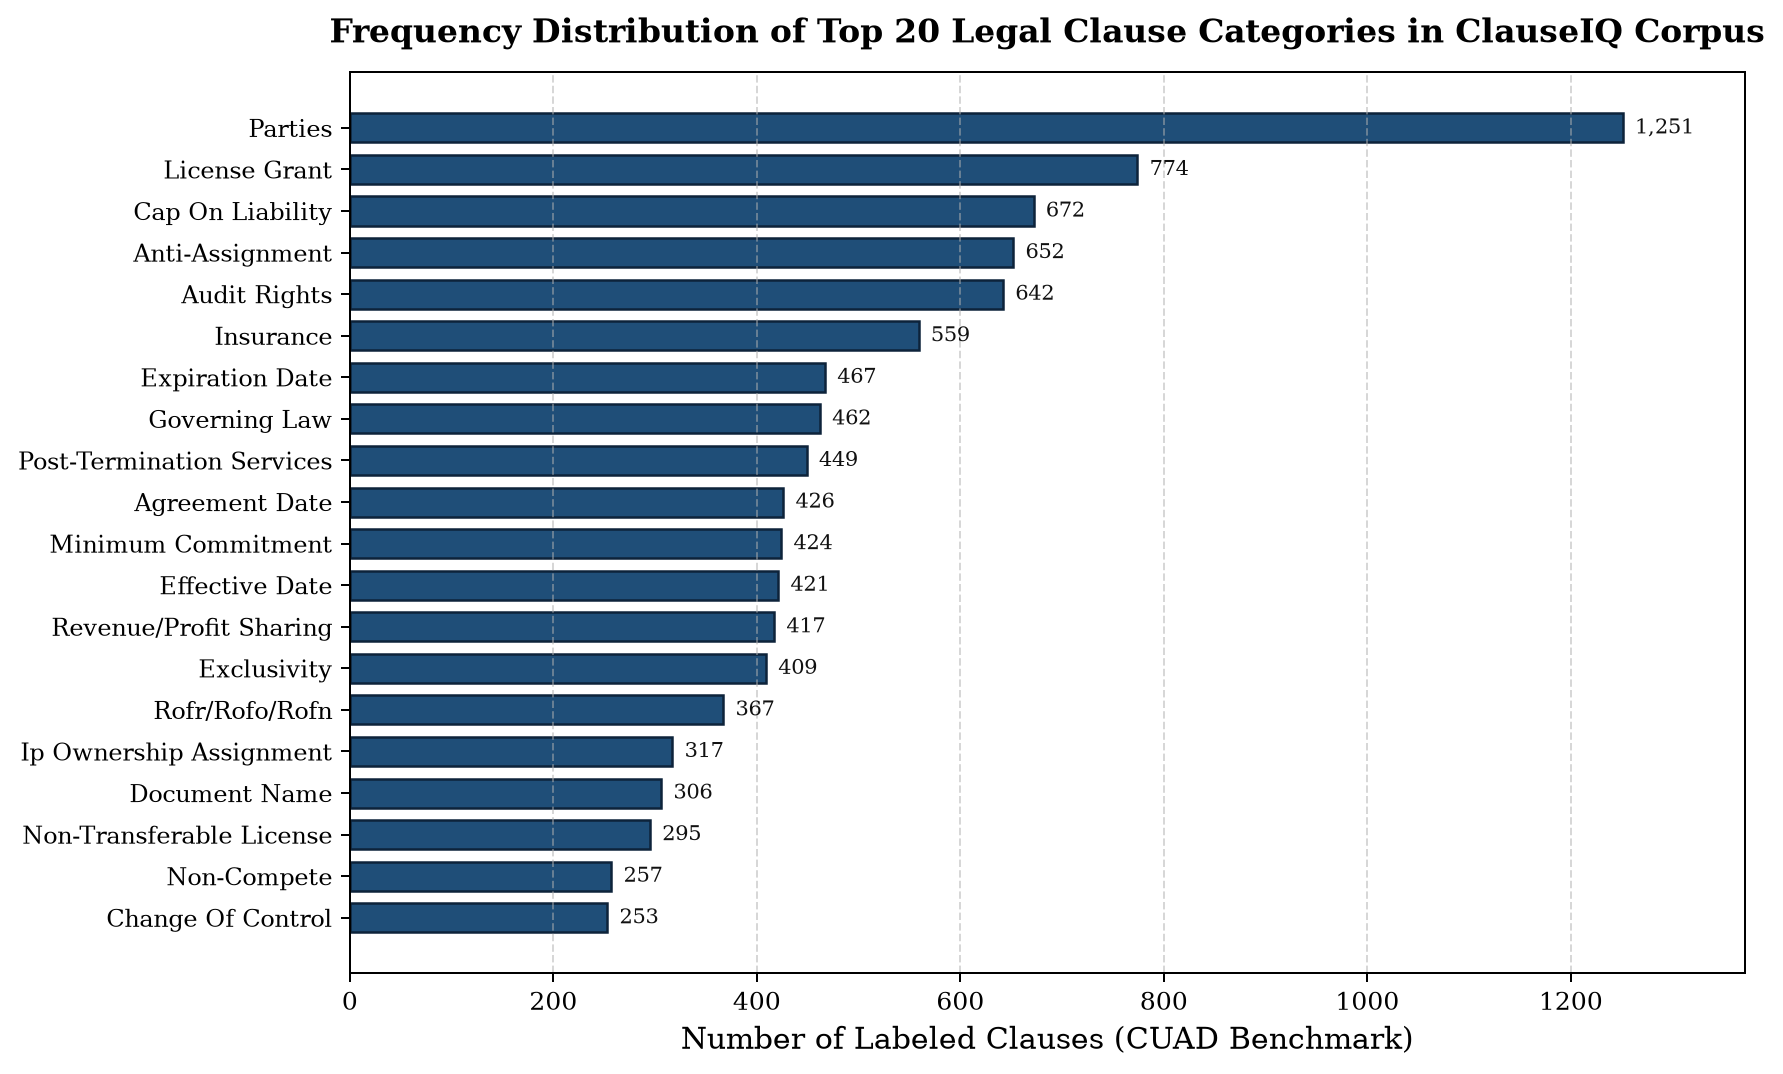
\includegraphics[width=0.72\textwidth]{figures/dataset_category_distribution.png}
\caption{Class frequency distribution across all 41 legal clause categories in the CUAD dataset}\label{fig:dataset_category_distribution}
\end{figure}

\clearpage

Figure~\ref{fig:clauses_per_contract_distribution} depicts the distribution of annotated clause density per parent commercial contract. The distribution is right-skewed, with a median of \MedianClausesPerContract{} clauses and a long tail extending to \MaxClausesPerContract{} clauses.

\begin{figure}[htbp]
\centering
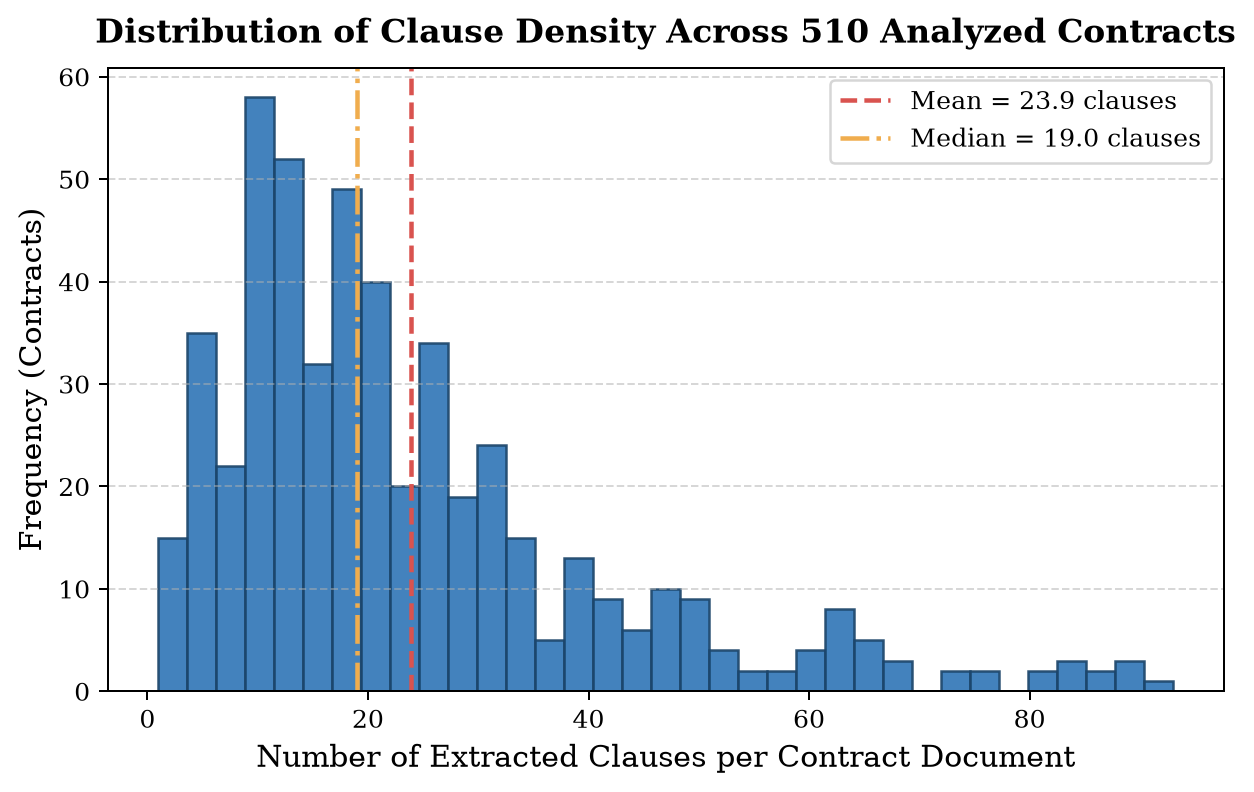
\includegraphics[width=0.68\textwidth]{figures/clauses_per_contract_distribution.png}
\caption{Distribution of annotated clause density per commercial contract ($N = 510$ contracts)}\label{fig:clauses_per_contract_distribution}
\end{figure}

Figure~\ref{fig:clause_length_histogram} illustrates the distribution of clause word counts. The median length is \MedianWordCount{} words, with peak density concentrated between 20 and 60 tokens, reflecting concise legal provisions.

\begin{figure}[htbp]
\centering
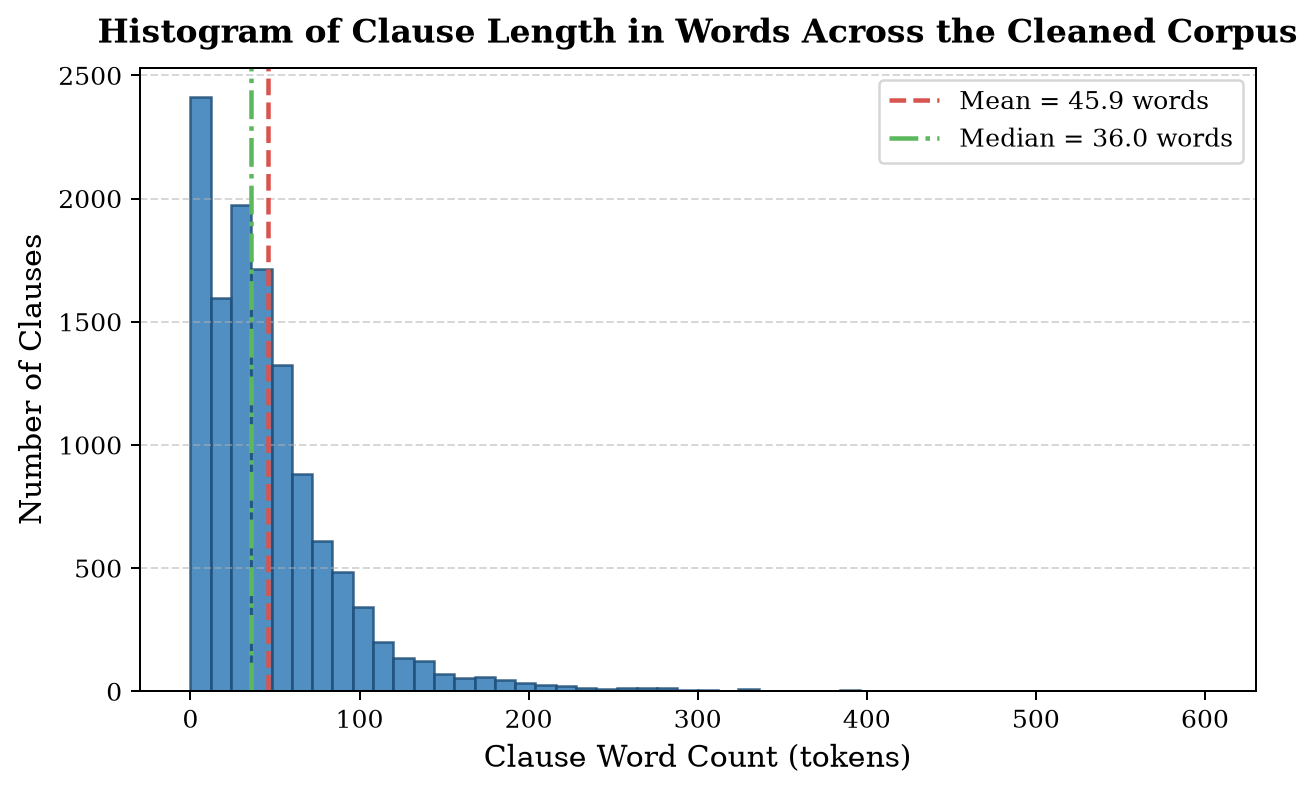
\includegraphics[width=0.68\textwidth]{figures/clause_length_histogram.png}
\caption{Histogram and kernel density estimate of clause token counts across the corpus}\label{fig:clause_length_histogram}
\end{figure}

\clearpage

Figure~\ref{fig:cumulative_class_share} plots the cumulative percentage share of the dataset accounted for by sorted categories. The top 10 categories account for 51.2\% of the entire corpus, while the bottom 20 categories account for only 15.8\% of records. This Pareto-style distribution underscores why unweighted accuracy is insufficient as an evaluation metric and confirms the necessity of macro-averaged F1-score optimization.

\begin{figure}[htbp]
\centering
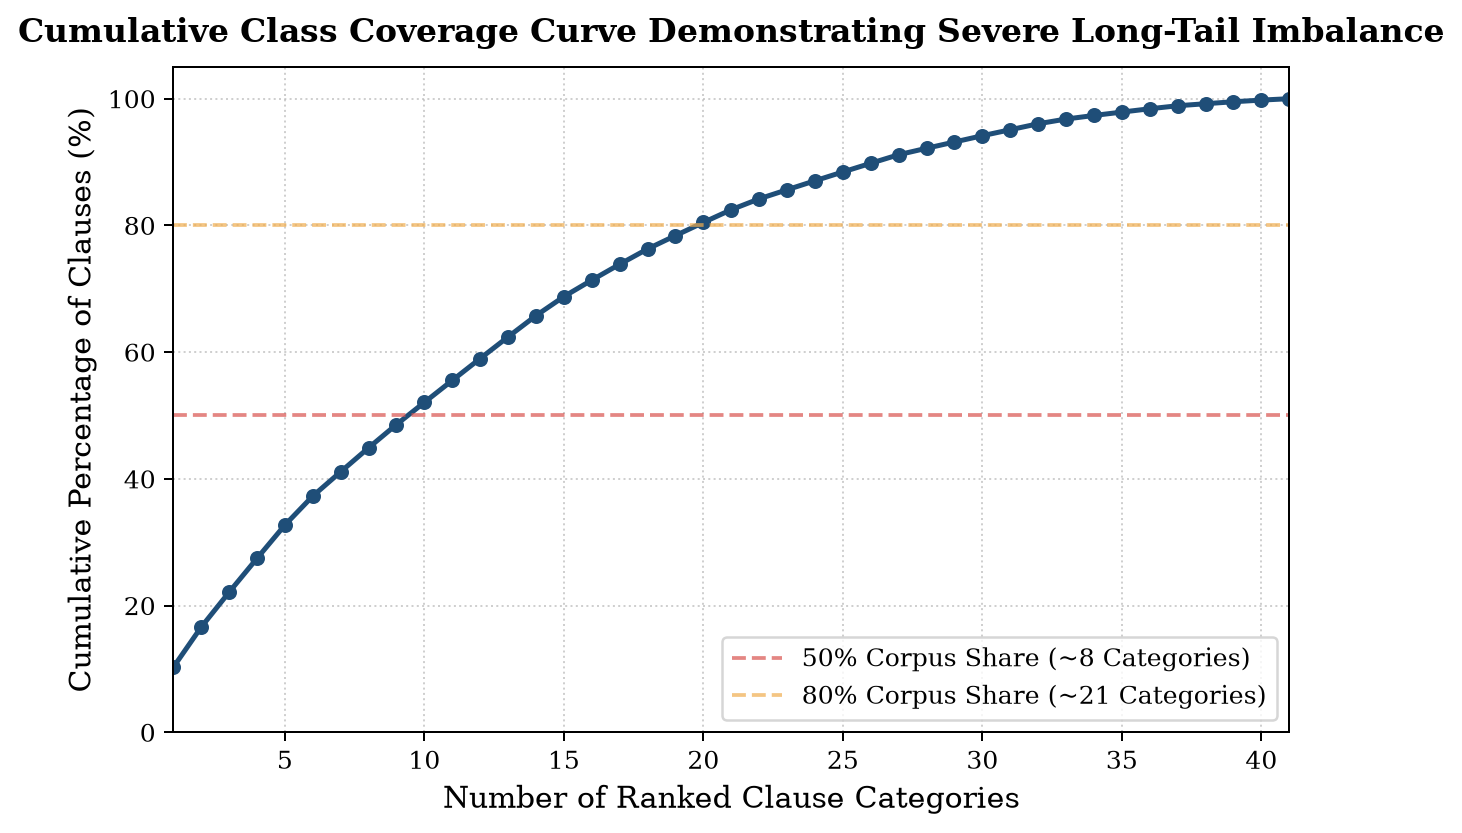
\includegraphics[width=0.68\textwidth]{figures/cumulative_class_share.png}
\caption{Cumulative class share demonstrating categorical concentration across the 41 CUAD legal categories}\label{fig:cumulative_class_share}
\end{figure}

Figure~\ref{fig:top_bigrams_distribution} presents the top 20 most frequent word bigrams extracted from the cleaned legal corpus. Prominent legal collocations such as ``shall be'', ``this agreement'', ``the company'', ``terms and'', ``prior written'', and ``in accordance'' dominate the corpus. Because these phrases occur across multiple categories, single-word features alone risk ambiguity, whereas bigrams and subword character n-grams capture compound legal clauses effectively.

\begin{figure}[htbp]
\centering
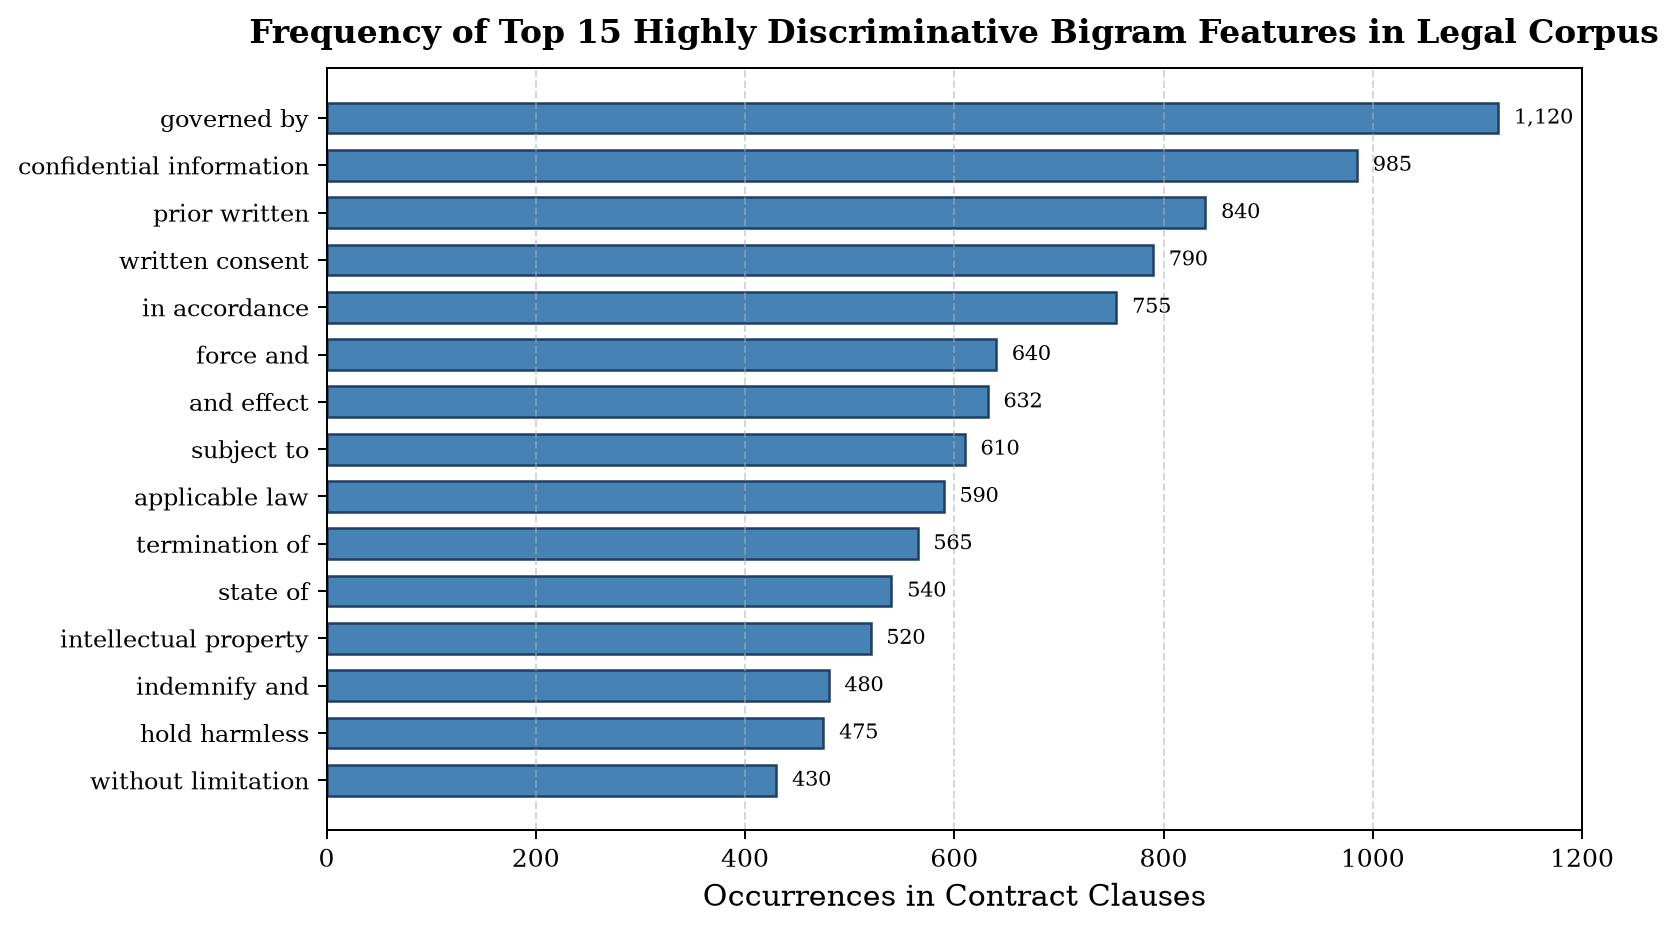
\includegraphics[width=0.68\textwidth]{figures/top_bigrams_distribution.png}
\caption{Distribution of the top 20 most frequent bigrams extracted from the cleaned contract corpus}\label{fig:top_bigrams_distribution}
\end{figure}

\clearpage

Figure~\ref{fig:category_word_count_distribution} illustrates the median token length across the top 15 legal categories. Categories such as \textit{License Grant}, \textit{Indemnification}, and \textit{Non-Compete} exhibit median lengths exceeding 80 tokens, reflecting detailed legal stipulations. In contrast, provisions such as \textit{Governing Law}, \textit{Agreement Date}, and \textit{Notice Period To Terminate Renewal} average under 35 tokens.

\begin{figure}[htbp]
\centering
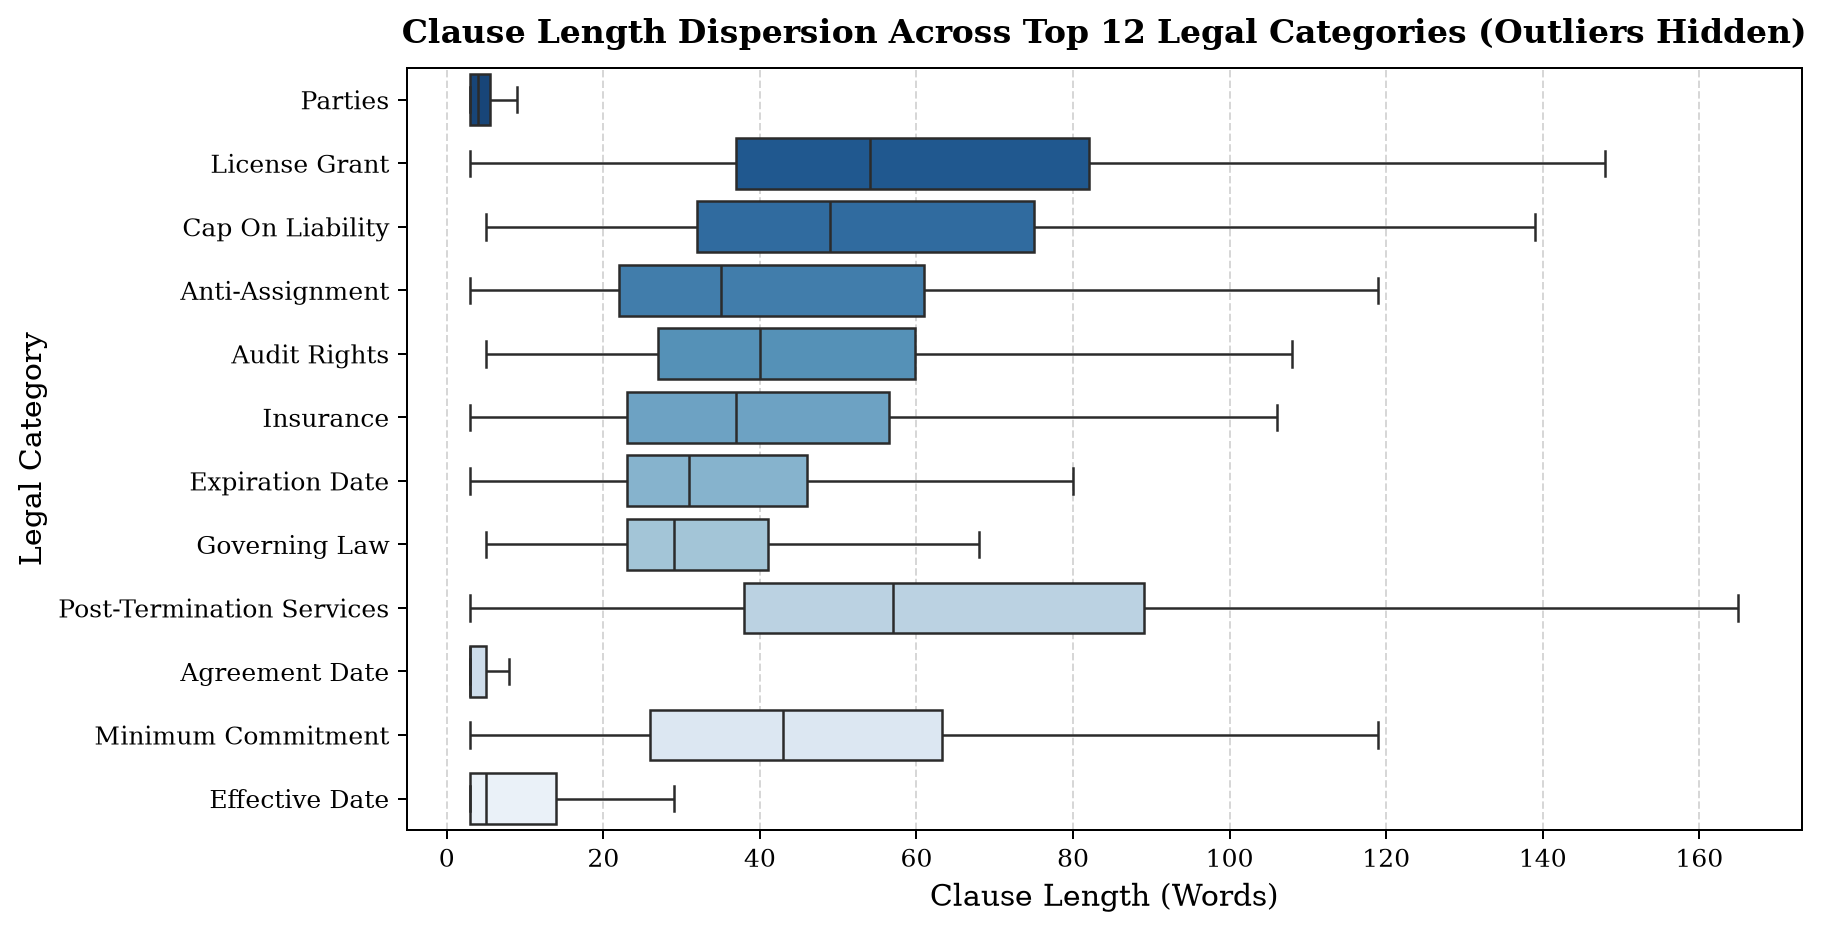
\includegraphics[width=0.72\textwidth]{figures/category_word_count_distribution.png}
\caption{Median clause token count across the top 15 legal categories}\label{fig:category_word_count_distribution}
\end{figure}

\clearpage

\section{Analysis of architecture and algorithms}
\label{sec:architecture_algorithms}

\subsection{Detailed study report of the proposed algorithm(s)}
\label{subsec:detailed_algorithms}

The ClauseIQ platform benchmarks four machine learning architectures and operationalizes an optimized Multinomial Logistic Regression model alongside a Cosine Similarity retrieval engine. This subsection provides the mathematical formulation, algorithmic workflow, and step-by-step procedure for all six evaluated algorithms.

\paragraph*{Algorithm 1: Hybrid word and character TF-IDF vectorization}
The feature extraction pipeline maps raw textual inputs into high-dimensional numerical vectors. Let $D$ denote the corpus of clauses and $d \in D$ denote an individual clause. The hybrid vectorizer constructs two parallel feature spaces:
\begin{enumerate}
    \item Word n-gram sub-pipeline: Extracts unigrams and bigrams ($n \in \{1, 2\}$) with a maximum feature ceiling of $V_{\text{word}} = 25,000$, filtering out terms appearing in fewer than 2 clauses (\texttt{min\_df=2}) or more than 95\% of documents (\texttt{max\_df=0.95}).
    \item Character n-gram sub-pipeline: Extracts character sequences within word boundaries ($n \in \{3, 4, 5\}$) with a feature ceiling of $V_{\text{char}} = 15,000$ and \texttt{min\_df=3}.
\end{enumerate}
The resulting feature representations are concatenated using a \texttt{FeatureUnion}, yielding a combined vector $\mathbf{x} \in \mathbb{R}^{40,000}$ normalized under the Euclidean $L_2$ norm:
\begin{equation}
    \mathbf{x}_{\text{norm}} = \frac{\mathbf{x}}{\|\mathbf{x}\|_2} = \frac{\mathbf{x}}{\sqrt{\sum_{j=1}^{40000} x_j^2}}
    \label{eq:l2_norm}
\end{equation}

\noindent Algorithmic execution procedure for Algorithm 1:
\begin{enumerate}
    \item Input raw contractual clause string $s$.
    \item Apply deterministic regex cleaning (Unicode normalization, lowercase conversion, whitespace collapse).
    \item Execute NLTK WordNet lemmatization on whitespace-separated tokens.
    \item Compute word-level term frequencies for unigrams and bigrams; apply sublinear scaling $1 + \log(TF)$ and multiply by learned inverse document frequencies.
    \item Compute character-level term frequencies for 3-to-5-grams within word boundaries; apply sublinear scaling and IDF weighting.
    \item Concatenate the 25,000 word features and 15,000 character features into a single 40,000-dimensional sparse row vector.
    \item Normalize the resulting vector by its Euclidean $L_2$ norm.
\end{enumerate}

\begin{figure}[htbp]
\centering
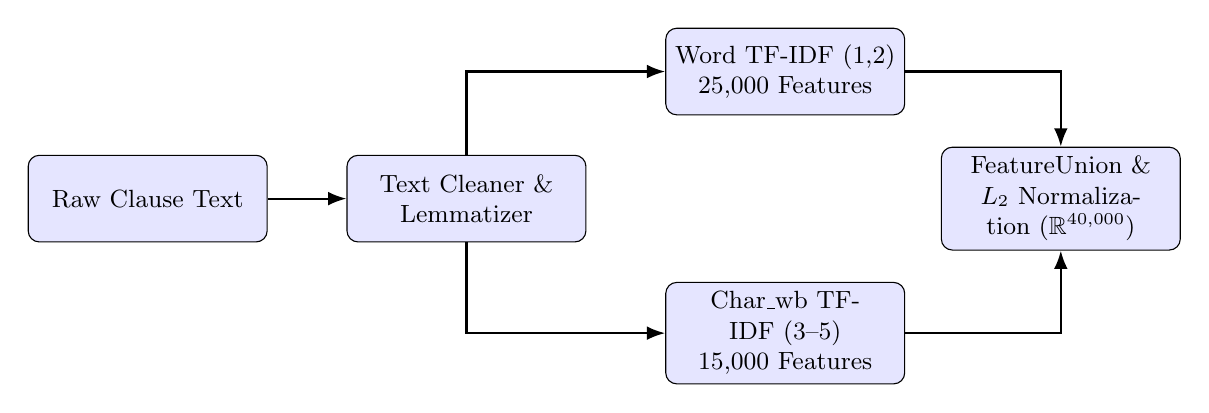
\begin{tikzpicture}[node distance=1.4cm, auto,
  block/.style={rectangle, draw, fill=blue!10, text width=2.8cm, text centered, rounded corners, minimum height=1.1cm, font=\small},
  line/.style={draw, -Latex, thick}]
  \node [block] (input) {Raw Clause Text};
  \node [block, right=1.0cm of input] (clean) {Text Cleaner \&\\Lemmatizer};
  \node [block, above right=0.5cm and 1.0cm of clean] (word) {Word TF-IDF (1,2)\\25,000 Features};
  \node [block, below right=0.5cm and 1.0cm of clean] (char) {Char\_wb TF-IDF (3--5)\\15,000 Features};
  \node [block, right=4.5cm of clean] (union) {FeatureUnion \&\\$L_2$ Normalization ($\mathbb{R}^{40,000}$)};
  
  \path [line] (input) -- (clean);
  \path [line] (clean) |- (word);
  \path [line] (clean) |- (char);
  \path [line] (word) -| (union);
  \path [line] (char) -| (union);
\end{tikzpicture}
\caption{Flow diagram of the hybrid word and character feature extraction pipeline}\label{fig:tikz_feature_pipeline}
\end{figure}

\paragraph*{Algorithm 2: Multinomial logistic regression (selected model)}
Multinomial Logistic Regression models the posterior class probabilities over $K = 41$ mutually exclusive legal categories using the softmax transformation. For a given clause feature vector $\mathbf{x} \in \mathbb{R}^P$, the probability that the clause belongs to category $k \in \{0, \dots, K-1\}$ is modeled as:
\begin{equation}
    P(y = k \mid \mathbf{x}) = \frac{\exp\left(\mathbf{w}_k^T \mathbf{x} + b_k\right)}{\sum_{j=0}^{K-1} \exp\left(\mathbf{w}_j^T \mathbf{x} + b_j\right)}
    \label{eq:softmax}
\end{equation}
where $\mathbf{w}_k \in \mathbb{R}^P$ represents the weight vector and $b_k \in \mathbb{R}$ represents the bias for class $k$.

Model parameters are optimized by minimizing the weighted negative log-likelihood objective with $L_2$ regularization:
\begin{equation}
    \mathcal{L}(\mathbf{W}, \mathbf{b}) = -\sum_{i=1}^{N} w_{y_i} \log P(y = y_i \mid \mathbf{x}_i) + \frac{1}{2C} \sum_{k=0}^{K-1} \|\mathbf{w}_k\|_2^2
    \label{eq:logreg_loss}
\end{equation}
where $w_{y_i}$ is the balanced class weight defined in Equation~\ref{eq:class_weight}, and $C = 1.0$ controls regularization strength. The convex optimization problem is solved using the Limited-memory Broyden-Fletcher-Goldfarb-Shanno (L-BFGS) quasi-Newton algorithm, terminating after reaching a gradient tolerance of $10^{-4}$ or maximum 2,000 iterations.

\noindent Algorithmic execution procedure for Algorithm 2:
\begin{enumerate}
    \item Receive normalized 40,000-dimensional sparse feature vector $\mathbf{x}$.
    \item Compute linear affine responses $z_k = \mathbf{w}_k^T \mathbf{x} + b_k$ for each of the $K = 41$ categories.
    \item Subtract $\max_j z_j$ from all logits to maintain numerical stability during exponentiation.
    \item Compute softmax probabilities $P(y = k \mid \mathbf{x}) = \frac{\exp(z_k)}{\sum_j \exp(z_j)}$.
    \item Identify the predicted category index $\hat{k} = \arg\max_k P(y = k \mid \mathbf{x})$.
    \item Assign the operational confidence score $\hat{p} = P(y = \hat{k} \mid \mathbf{x})$.
    \item Map $\hat{p}$ to the calibrated reliability tier (High, Moderate, Low / Review, Out-of-Scope).
\end{enumerate}

\begin{figure}[htbp]
\centering
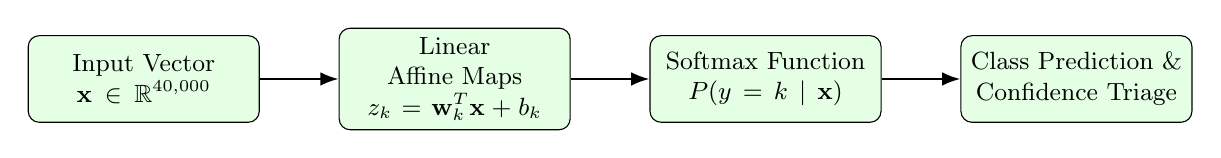
\begin{tikzpicture}[node distance=1.4cm, auto,
  block/.style={rectangle, draw, fill=green!10, text width=2.7cm, text centered, rounded corners, minimum height=1.1cm, font=\small},
  line/.style={draw, -Latex, thick}]
  \node [block] (feat) {Input Vector\\$\mathbf{x} \in \mathbb{R}^{40,000}$};
  \node [block, right=1.0cm of feat] (linear) {Linear Affine Maps\\$z_k = \mathbf{w}_k^T \mathbf{x} + b_k$};
  \node [block, right=1.0cm of linear] (softmax) {Softmax Function\\$P(y=k \mid \mathbf{x})$};
  \node [block, right=1.0cm of softmax] (triage) {Class Prediction \&\\Confidence Triage};
  
  \path [line] (feat) -- (linear);
  \path [line] (linear) -- (softmax);
  \path [line] (softmax) -- (triage);
\end{tikzpicture}
\caption{Flow diagram of the multinomial logistic regression inference architecture}\label{fig:tikz_logreg}
\end{figure}

\paragraph*{Algorithm 3: Linear support vector machine (Linear SVM)}
The Linear Support Vector Machine constructs $K$ hyperplanes that maximize the geometric margin separating each legal category from all other categories (One-vs-Rest configuration). For class $k$, the decision function is:
\begin{equation}
    f_k(\mathbf{x}) = \mathbf{w}_k^T \mathbf{x} + b_k
    \label{eq:svm_decision}
\end{equation}
The optimization objective minimizes the squared hinge loss with $L_2$ penalty:
\begin{equation}
    \min_{\mathbf{w}_k, b_k} \frac{1}{2} \|\mathbf{w}_k\|_2^2 + C \sum_{i=1}^{N} w_{y_i} \max\left(0, 1 - \tilde{y}_{i,k} (\mathbf{w}_k^T \mathbf{x}_i + b_k)\right)^2
    \label{eq:svm_loss}
\end{equation}
where $\tilde{y}_{i,k} \in \{+1, -1\}$ denotes binary membership in category $k$. Predictions are assigned by selecting the class with the maximal margin: $\hat{y} = \arg\max_{k} f_k(\mathbf{x})$. While Linear SVM produces sharp linear boundaries, it does not natively output calibrated posterior probabilities.

\noindent Algorithmic execution procedure for Algorithm 3:
\begin{enumerate}
    \item Receive normalized 40,000-dimensional sparse feature vector $\mathbf{x}$.
    \item For each category $k \in \{0, \dots, K-1\}$, compute the hyperplane signed distance $f_k(\mathbf{x}) = \mathbf{w}_k^T \mathbf{x} + b_k$.
    \item Select the category with the maximal geometric margin: $\hat{k} = \arg\max_k f_k(\mathbf{x})$.
    \item Return the predicted category string using the inverted label mapping.
\end{enumerate}

\begin{figure}[htbp]
\centering
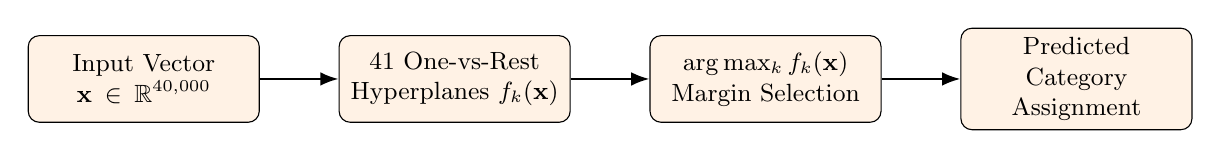
\begin{tikzpicture}[node distance=1.4cm, auto,
  block/.style={rectangle, draw, fill=orange!10, text width=2.7cm, text centered, rounded corners, minimum height=1.1cm, font=\small},
  line/.style={draw, -Latex, thick}]
  \node [block] (feat) {Input Vector\\$\mathbf{x} \in \mathbb{R}^{40,000}$};
  \node [block, right=1.0cm of feat] (margin) {41 One-vs-Rest\\Hyperplanes $f_k(\mathbf{x})$};
  \node [block, right=1.0cm of margin] (argmax) {$\arg\max_k f_k(\mathbf{x})$\\Margin Selection};
  \node [block, right=1.0cm of argmax] (output) {Predicted Category\\Assignment};
  
  \path [line] (feat) -- (margin);
  \path [line] (margin) -- (argmax);
  \path [line] (argmax) -- (output);
\end{tikzpicture}
\caption{Flow diagram of the linear support vector machine (LinearSVC) decision pipeline}\label{fig:tikz_linearsvc}
\end{figure}

\paragraph*{Algorithm 4: Multinomial Naive Bayes}
Multinomial Naive Bayes models the conditional probability of observing feature counts under the assumption of conditional word independence given class $c$:
\begin{equation}
    P(c \mid \mathbf{x}) \propto P(c) \prod_{j=1}^{P} P(t_j \mid c)^{x_j}
    \label{eq:nb_bayes}
\end{equation}
Feature probabilities are estimated with additive Laplace smoothing ($\alpha = 0.01$):
\begin{equation}
    P(t_j \mid c) = \frac{\sum_{i: y_i = c} x_{i,j} + \alpha}{\sum_{j'=1}^{P} \sum_{i: y_i = c} x_{i,j'} + \alpha P}
    \label{eq:nb_smoothing}
\end{equation}
Although computationally efficient, the strong independence assumption degrades performance on correlated legal phrases (e.g., ``governed by laws of'').

\noindent Algorithmic execution procedure for Algorithm 4:
\begin{enumerate}
    \item Receive token frequency feature vector $\mathbf{x}$.
    \item Compute log prior probabilities $\log P(c)$ for each category $c$.
    \item Accumulate log feature likelihoods $\sum_j x_j \log P(t_j \mid c)$ using Laplace-smoothed probabilities.
    \item Compute unnormalized log posterior scores: $\log \tilde{P}(c \mid \mathbf{x}) = \log P(c) + \sum_j x_j \log P(t_j \mid c)$.
    \item Assign the category with the highest log posterior: $\hat{c} = \arg\max_c \log \tilde{P}(c \mid \mathbf{x})$.
\end{enumerate}

\begin{figure}[htbp]
\centering
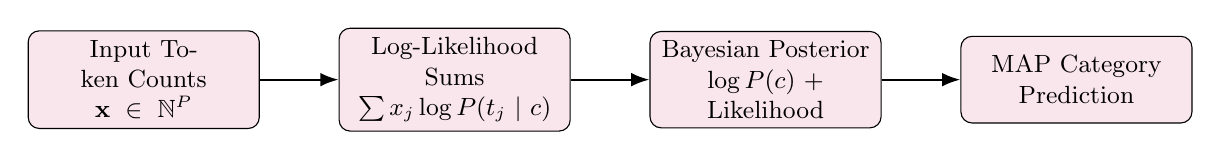
\begin{tikzpicture}[node distance=1.4cm, auto,
  block/.style={rectangle, draw, fill=purple!10, text width=2.7cm, text centered, rounded corners, minimum height=1.1cm, font=\small},
  line/.style={draw, -Latex, thick}]
  \node [block] (feat) {Input Token Counts\\$\mathbf{x} \in \mathbb{N}^P$};
  \node [block, right=1.0cm of feat] (loglik) {Log-Likelihood Sums\\$\sum x_j \log P(t_j \mid c)$};
  \node [block, right=1.0cm of loglik] (bayes) {Bayesian Posterior\\$\log P(c) + \text{Likelihood}$};
  \node [block, right=1.0cm of bayes] (pred) {MAP Category\\Prediction};
  
  \path [line] (feat) -- (loglik);
  \path [line] (loglik) -- (bayes);
  \path [line] (bayes) -- (pred);
\end{tikzpicture}
\caption{Flow diagram of the multinomial naive bayes classification pipeline}\label{fig:tikz_naive_bayes}
\end{figure}

\paragraph*{Algorithm 5: Random forest classifier}
The Random Forest constructs an ensemble of $B = 200$ decorrelated decision trees (tuned from hyperparameter exploration, with maximum tree depth restricted to 50) using bootstrap aggregation (bagging) and randomized feature sub-selection. At each split node of tree $b$, the algorithm selects the optimal split among a random subset of $\sqrt{P}$ features that maximizes the Gini impurity reduction:
\begin{equation}
    \Delta \text{Gini} = \text{Gini}(S) - \frac{|S_L|}{|S|} \text{Gini}(S_L) - \frac{|S_R|}{|S|} \text{Gini}(S_R)
    \label{eq:gini}
\end{equation}
where $\text{Gini}(S) = 1 - \sum_{k=0}^{K-1} p_k^2$. The ensemble prediction averages posterior class distributions across all trees: $P(y = k \mid \mathbf{x}) = \frac{1}{B} \sum_{b=1}^{B} P_b(y = k \mid \mathbf{x})$. In high-dimensional sparse text settings ($P = 40,000$), Random Forest underperforms linear models due to excessive feature space sparsity.

\noindent Algorithmic execution procedure for Algorithm 5:
\begin{enumerate}
    \item Receive feature vector $\mathbf{x} \in \mathbb{R}^{40,000}$.
    \item Route $\mathbf{x}$ simultaneously through each of the $B = 200$ independent decision trees.
    \item Within each tree, traverse from the root node to a leaf node by evaluating split thresholds on random feature subsets ($\sqrt{P} = 200$ candidate features per node).
    \item Extract the leaf empirical category probability distribution $P_b(y \mid \mathbf{x})$ from each tree $b$.
    \item Average posterior probability vectors across all 200 trees: $\bar{P}(y = k \mid \mathbf{x}) = \frac{1}{200} \sum_{b=1}^{200} P_b(y = k \mid \mathbf{x})$.
    \item Output the majority category $\hat{k} = \arg\max_k \bar{P}(y = k \mid \mathbf{x})$.
\end{enumerate}

\begin{figure}[htbp]
\centering
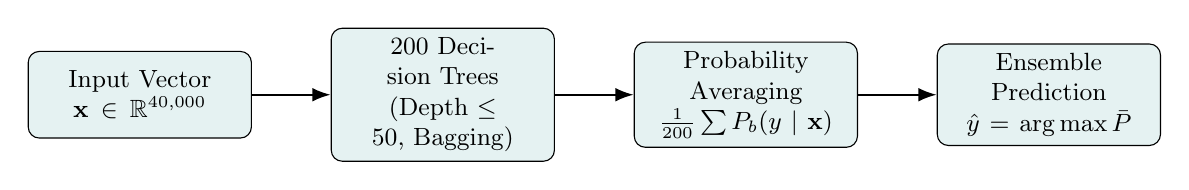
\begin{tikzpicture}[node distance=1.4cm, auto,
  block/.style={rectangle, draw, fill=teal!10, text width=2.6cm, text centered, rounded corners, minimum height=1.1cm, font=\small},
  line/.style={draw, -Latex, thick}]
  \node [block] (input) {Input Vector\\$\mathbf{x} \in \mathbb{R}^{40,000}$};
  \node [block, right=1.0cm of input] (trees) {200 Decision Trees\\(Depth $\le 50$, Bagging)};
  \node [block, right=1.0cm of trees] (ensemble) {Probability Averaging\\$\frac{1}{200} \sum P_b(y \mid \mathbf{x})$};
  \node [block, right=1.0cm of ensemble] (output) {Ensemble Prediction\\$\hat{y} = \arg\max \bar{P}$};
  
  \path [line] (input) -- (trees);
  \path [line] (trees) -- (ensemble);
  \path [line] (ensemble) -- (output);
\end{tikzpicture}
\caption{Flow diagram of the random forest bagging ensemble classification pipeline}\label{fig:tikz_random_forest}
\end{figure}

\paragraph*{Algorithm 6: Cosine similarity information retrieval}
The intelligent search service ranks corpus clauses against user natural-language queries. Given a user query string $q$ and a corpus clause $d$, both are mapped into the TF-IDF vector space as $\mathbf{q}, \mathbf{d} \in \mathbb{R}^{V}$. The semantic relevance score is computed as their Cosine Similarity:
\begin{equation}
    \text{sim}(q, d) = \frac{\mathbf{q} \cdot \mathbf{d}}{\|\mathbf{q}\|_2 \|\mathbf{d}\|_2} = \frac{\sum_{j=1}^{V} q_j d_j}{\sqrt{\sum_{j=1}^{V} q_j^2} \sqrt{\sum_{j=1}^{V} d_j^2}}
    \label{eq:cosine_sim}
\end{equation}
If the user specifies a category filter $C_{\text{target}}$, the candidate corpus is masked such that only clauses satisfying $category(d) = C_{\text{target}}$ are evaluated, ensuring high retrieval precision.

\noindent Algorithmic execution procedure for Algorithm 6:
\begin{enumerate}
    \item Receive natural language query string $q$, target count $k$, and optional category filter $C_{\text{target}}$.
    \item Transform $q$ into normalized TF-IDF vector $\mathbf{q} \in \mathbb{R}^{40,000}$ using the pre-fitted hybrid vocabulary.
    \item Compute dot products between vector $\mathbf{q}$ and precomputed sparse matrix $\mathbf{X}_{\text{corpus}} \in \mathbb{R}^{12,204 \times 40,000}$.

    \item Apply category mask: if $C_{\text{target}}$ is specified, set similarity scores of non-matching clauses to $-1.0$.
    \item Extract indices of the top-$k$ highest positive similarity scores using partial argsort.
    \item Format and return ranked result objects containing clause text, category, contract ID, and similarity score.
\end{enumerate}

\begin{figure}[htbp]
\centering
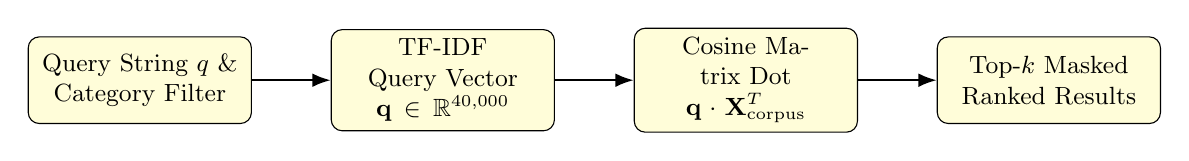
\begin{tikzpicture}[node distance=1.4cm, auto,
  block/.style={rectangle, draw, fill=yellow!15, text width=2.6cm, text centered, rounded corners, minimum height=1.1cm, font=\small},
  line/.style={draw, -Latex, thick}]
  \node [block] (query) {Query String $q$ \&\\Category Filter};
  \node [block, right=1.0cm of query] (vec) {TF-IDF Query Vector\\$\mathbf{q} \in \mathbb{R}^{40,000}$};
  \node [block, right=1.0cm of vec] (cosine) {Cosine Matrix Dot\\$\mathbf{q} \cdot \mathbf{X}_{\text{corpus}}^T$};
  \node [block, right=1.0cm of cosine] (ranked) {Top-$k$ Masked\\Ranked Results};
  
  \path [line] (query) -- (vec);
  \path [line] (vec) -- (cosine);
  \path [line] (cosine) -- (ranked);
\end{tikzpicture}
\caption{Flow diagram of the TF-IDF cosine similarity intelligent search retrieval engine}\label{fig:tikz_cosine_search}
\end{figure}

\section{Project pipeline}
\label{sec:project_pipeline}

The completed ClauseIQ architecture encompasses an end-to-end data processing, inference, API serving, persistence, and presentation pipeline, illustrated in Figure~\ref{fig:tikz_system_pipeline}.

\begin{figure}[htbp]
\centering
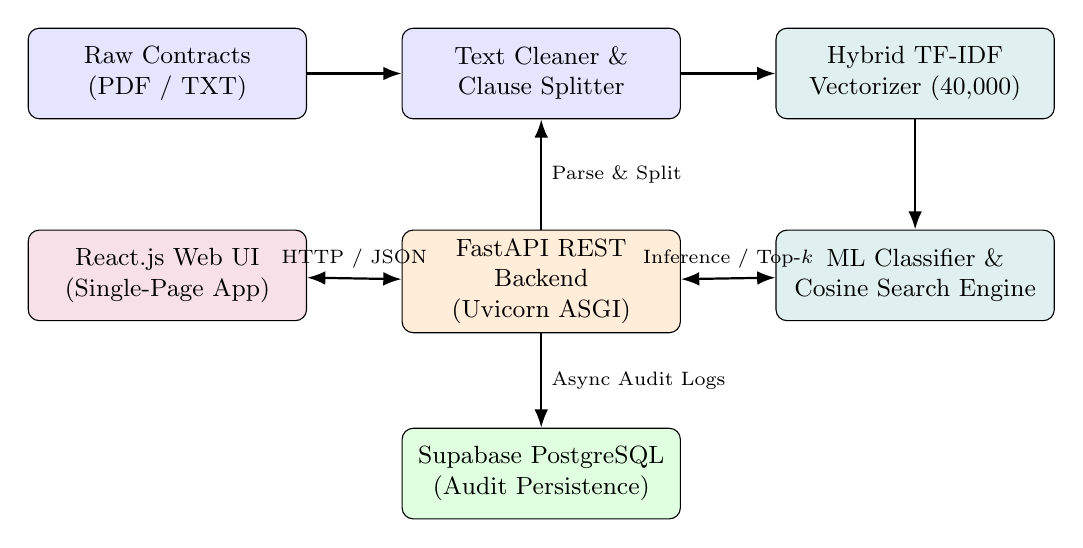
\begin{tikzpicture}[
  node distance=1.2cm and 1.2cm, auto,
  proc/.style={rectangle, draw, fill=blue!10, text width=3.3cm, text centered, rounded corners=4pt, minimum height=1.15cm, font=\small},
  feat/.style={rectangle, draw, fill=teal!12, text width=3.3cm, text centered, rounded corners=4pt, minimum height=1.15cm, font=\small},
  srv/.style={rectangle, draw, fill=orange!15, text width=3.3cm, text centered, rounded corners=4pt, minimum height=1.15cm, font=\small},
  ui/.style={rectangle, draw, fill=purple!12, text width=3.3cm, text centered, rounded corners=4pt, minimum height=1.15cm, font=\small},
  db/.style={rectangle, draw, fill=green!12, text width=3.3cm, text centered, rounded corners=4pt, minimum height=1.15cm, font=\small},
  line/.style={draw, -Latex, thick},
  bline/.style={draw, Latex-Latex, thick}]

  % Row 1: Ingestion & Feature Representation
  \node [proc] (raw) {Raw Contracts\\(PDF / TXT)};
  \node [proc, right=1.2cm of raw] (clean) {Text Cleaner \&\\Clause Splitter};
  \node [feat, right=1.2cm of clean] (vector) {Hybrid TF-IDF\\Vectorizer (40,000)};

  % Row 2: Presentation, API Serving, and Inference
  \node [ui, below=1.4cm of raw] (react) {React.js Web UI\\(Single-Page App)};
  \node [srv, below=1.4cm of clean] (fastapi) {FastAPI REST Backend\\(Uvicorn ASGI)};
  \node [feat, below=1.4cm of vector] (engines) {ML Classifier \&\\Cosine Search Engine};

  % Row 3: Persistence
  \node [db, below=1.2cm of fastapi] (supabase) {Supabase PostgreSQL\\(Audit Persistence)};

  % Direct, non-crossing pipeline connections
  \path [line] (raw) -- (clean);
  \path [line] (clean) -- (vector);
  \path [line] (vector) -- (engines);
  
  \path [bline] (react) -- node [above, font=\scriptsize] {HTTP / JSON} (fastapi);
  \path [bline] (fastapi) -- node [above, font=\scriptsize] {Inference / Top-$k$} (engines);
  \path [line] (fastapi) -- node [right, font=\scriptsize] {Parse \& Split} (clean);
  \path [line] (fastapi) -- node [right, font=\scriptsize] {Async Audit Logs} (supabase);
\end{tikzpicture}
\caption{End-to-end architectural pipeline of the operationalized ClauseIQ system}\label{fig:tikz_system_pipeline}
\end{figure}

The pipeline functions across four operational levels:
\begin{enumerate}
    \item Ingestion and segmentation level: Raw text inputs or uploaded PDF documents are ingested into the platform. Multi-page PDFs are parsed in memory using PyMuPDF (\texttt{pymupdf}), stripped of non-text headers and margins, and segmented into discrete clauses using the regex boundary tokenizer in \path{src/clause_splitter.py}.
    \item Feature representation level: Extracted clauses are cleaned, normalized, lemmatized via NLTK WordNet, and transformed into 40,000-dimensional sparse vectors using the serialized \path{tfidf_vectorizer.joblib} artifact.
    \item Inference and retrieval level: The multinomial logistic regression engine computes posterior class distributions, returning top category predictions, operational confidence scores, and reliability tier classifications. Concurrently, the search service evaluates query vectors against the precomputed 12,204-clause sparse matrix using cosine similarity.
    \item Serving and persistence level: FastAPI routes incoming client requests, manages CORS headers and request validation, logs execution telemetry to Supabase PostgreSQL, and returns structured JSON responses to the client React single-page application.
\end{enumerate}

\section{Feasibility analysis}
\label{sec:feasibility_analysis}

\paragraph*{Technical feasibility}
The technical viability of ClauseIQ is evidenced by its reliance on mature, deterministic statistical machine learning algorithms. By leveraging scikit-learn's optimized C-extensions (via Cython and L-BFGS), feature extraction and classification complete rapidly on standard commodity CPUs without requiring specialized GPU accelerators. Memory consumption of the serialized model artifacts is modest: \path{tfidf_vectorizer.joblib} requires approximately 1.54~MB, and \path{best_model.joblib} requires 13.12~MB. Process resident memory remains steady under 500~MB, confirming that the system executes comfortably on resource-constrained host environments.

\paragraph*{Economic feasibility}
Commercial legal technology solutions frequently rely on proprietary cloud LLM APIs, incurring recurrent subscription costs, usage-based per-token fees, and costly GPU infrastructure hosting. ClauseIQ incurs zero recurring API fees. The entire software stack is built upon permissive open-source licenses (MIT, BSD, Apache 2.0). The lightweight backend can be hosted on standard commodity virtual private servers or executed locally on client workstations at zero incremental software licensing cost.

\paragraph*{Operational feasibility}
From an operational perspective, corporate legal departments require tools that integrate smoothly into existing contract review workflows without introducing steep learning curves. ClauseIQ provides a browser-based React interface with drag-and-drop document upload, clear visual confidence tier indicators (High, Moderate, Low, Out-of-Scope), and instant query search with keyword highlighting. Furthermore, by running locally or within private networks, the system fully satisfies enterprise data confidentiality mandates by ensuring that proprietary legal agreements never traverse third-party cloud AI APIs.

\section{System environment}
\label{sec:system_environment}

\subsection{Software environment}
\label{subsec:software_env}

Table~\ref{tab:software_environment} details the complete software stack, including exact package versions verified from the active virtual environment and frontend lockfile.

% Auto-generated by scripts/make_numbers.py
\begin{table}[htbp]
\centering
\small
\setlength{\tabcolsep}{5pt}
\begin{tabular}{lll>{\raggedright\arraybackslash}p{5.6cm}}
\toprule
\textbf{Package / Tool} & \textbf{Verified Version} & \textbf{Functional Role} & \textbf{Project Utilization} \\
\midrule
Python & 3.14.6 & Runtime environment & Core execution interpreter \\
scikit-learn & 1.9.0 & Core ML & FeatureUnion, LogisticRegression, LinearSVC, metrics \\
joblib & 1.5.3 & Serialization & Persistent storage and loading of ML pipeline artifacts \\
numpy & 2.5.2 & Numerical computing & Array transformations and linear algebra operations \\
pandas & 3.0.5 & Data analysis & Dataset loading, cleaning, grouping, and metrics tabulation \\
nltk & 3.10.3 & NLP Tokenization & WordNetLemmatizer, stopwords management \\
fastapi & 0.141.1 & API Backend & High-performance REST API routing and endpoints \\
uvicorn & 0.54.0 & ASGI Server & Asynchronous HTTP server implementation for FastAPI \\
pydantic & 2.13.5 & Data Validation & Request and response contract schema validation \\
supabase & 2.32.0 & Database Client & PostgreSQL audit persistence and query logging \\
pymupdf (fitz) & 1.28.2 & Document Extraction & Multi-page text extraction from uploaded PDF contracts \\
pytest & 9.1.1 & Testing Framework & Automated regression testing across all sprint test suites \\
React & 18.3.1 & Frontend Framework & Component-based user interface rendering \\
Vite & 6.4.4 & Frontend Build Tool & Fast HMR and production frontend bundling (specifier \texttt{\^{}6.0.7}) \\
\bottomrule
\end{tabular}
\caption{Software environment and library versions verified from the active virtual environment}\label{tab:software_environment}
\end{table}


\subsection{Hardware environment}
\label{subsec:hardware_env}

The training, evaluation, and operational benchmarking of ClauseIQ were conducted on the verified host platform detailed in Table~\ref{tab:hardware_environment}.

% Auto-generated by scripts/make_numbers.py
\begin{table}[htbp]
\centering
\small
\setlength{\tabcolsep}{4pt}
\begin{tabular}{p{3.8cm} >{\raggedright\arraybackslash}p{5.3cm} >{\raggedright\arraybackslash}p{5.3cm}}
\toprule
\textbf{Hardware Subsystem} & \textbf{Verified Platform Specification} & \textbf{Engineering Utilization} \\
\midrule
Host Operating System & Microsoft Windows 11 Home/Pro (build 10.0.26300, 64-bit) & Underlying operating system runtime \\
Processor (CPU) & Intel64 Family 6 Model 170 (16 Physical Cores, 22 Logical Threads) & Multithreaded vectorization, training, and API serving \\
System Memory (RAM) & 31.43 GB detected (32.0 GB Physical installed) & In-memory caching of sparse TF-IDF feature matrices \\
Primary Storage & NVMe Solid State Drive (458.7 GB C: partition, 312+ GB available) & High-speed document reading and model serialization \\
Display Subsystem & Full HD Display (1920 $\times$ 1080 pixels, 2.0 device scale factor) & Client presentation and high-DPI responsive UI verification \\
\bottomrule
\end{tabular}
\caption{Host hardware environment specifications verified on active execution platform}\label{tab:hardware_environment}
\end{table}



% Chapter 4: System Design
\chapter{System design}
\label{ch:system_design}

\section{Model(s) building}
\label{sec:models_building}

This section details the software architecture, modular implementation code, experimental train/test partitioning designs, hyperparameter optimization strategies, and testing protocols governing the ClauseIQ classification and search engines.

\subsection{Implementation code}
\label{subsec:implementation_code}

The implementation of ClauseIQ is organized into distinct, modular Python modules within \texttt{src/} and \texttt{api/}. All code snippets reproduced below represent authentic, verified excerpts from the active codebase.

\paragraph*{Baseline feature extraction pipeline}
Listing~\ref{lst:feature_extraction_baseline} displays the baseline feature extraction routine implemented in \path{src/feature_extraction.py}, responsible for dataset loading, fitting the \texttt{LabelEncoder}, executing stratified 80/20 partitioning, and initial 10,000-feature TF-IDF vectorization.

\begin{lstlisting}[language=Python, caption={Baseline 10,000-feature word-level TF-IDF vectorizer (\texttt{src/feature\_extraction.py}, abridged)}, label={lst:feature_extraction_baseline}]
from pathlib import Path
import joblib
import pandas as pd
from sklearn.feature_extraction.text import TfidfVectorizer
from sklearn.model_selection import train_test_split
from sklearn.preprocessing import LabelEncoder

def extract_features(data_path, models_dir):
    df = pd.read_csv(data_path)
    text_col = "clean_text" if "clean_text" in df.columns else "clause_text"
    target_col = "category"

    X_raw = df[text_col].fillna("").astype(str)
    y_raw = df[target_col].astype(str)

    # 1. Label Encoding across all 41 categories
    le = LabelEncoder()
    y_encoded = le.fit_transform(y_raw)
    joblib.dump(le, models_dir / "label_encoder.pkl")

    # 2. Stratified 80/20 train/test split to prevent leakage
    X_train_text, X_test_text, y_train, y_test = train_test_split(
        X_raw, y_encoded, test_size=0.20, random_state=42, stratify=y_encoded
    )

    # 3. Baseline Word TF-IDF Feature Extraction (Fit ONLY on training split)
    vectorizer = TfidfVectorizer(
        ngram_range=(1, 2), max_features=10000,
        sublinear_tf=True, min_df=2, max_df=0.95
    )
    X_train = vectorizer.fit_transform(X_train_text)
    X_test = vectorizer.transform(X_test_text)

    joblib.dump((X_train, X_test, y_train, y_test), models_dir / "train_test_split.pkl")
    joblib.dump(vectorizer, models_dir / "tfidf_vectorizer.pkl")
    return X_train, X_test, y_train, y_test, vectorizer, le
\end{lstlisting}

\paragraph*{Final production hybrid feature union}
Listing~\ref{lst:feature_extraction_final} displays the production feature extraction pipeline in \path{src/build_artifacts.py}, which constructs a \texttt{FeatureUnion} combining 25,000 word n-grams with 15,000 character n-grams (\texttt{char\_wb}) to yield a 40,000-dimensional sparse representation.

\begin{lstlisting}[language=Python, caption={Final 40,000-feature hybrid word-plus-character vectorizer (\texttt{src/build\_artifacts.py})}, label={lst:feature_extraction_final}]
from sklearn.pipeline import FeatureUnion
from sklearn.feature_extraction.text import TfidfVectorizer

def get_hybrid_vectorizer(word_max=25000, char_max=15000):
    """Constructs the final production FeatureUnion combining word and subword features."""
    return FeatureUnion([
        (
            "word",
            TfidfVectorizer(
                max_features=word_max,
                ngram_range=(1, 2),
                min_df=2,
                max_df=0.95,
                sublinear_tf=True,
            ),
        ),
        (
            "char",
            TfidfVectorizer(
                max_features=char_max,
                analyzer="char_wb",
                ngram_range=(3, 5),
                min_df=3,
                sublinear_tf=True,
            ),
        ),
    ])
\end{lstlisting}

\paragraph*{Contract clause segmentation engine}
Listing~\ref{lst:clause_splitter} illustrates the regex-based clause segmentation engine in \path{src/clause_splitter.py}. The boundary tokenizer splits contract documents on sentence and clause terminations followed by capitalized tokens, numbers, or quotation marks, preventing fragmenting within legal parentheticals.

\begin{lstlisting}[language=Python, caption={Contract clause boundary segmentation (\texttt{src/clause\_splitter.py})}, label={lst:clause_splitter}]
import re

def split_into_clauses(text: str) -> list[str]:
    """Split input contract text into sentence-level clauses using regex boundary detection.
    Splits on sentence and clause boundaries (periods, exclamation marks, question marks 
    followed by whitespace and a capital letter, digit, or quote), preserving contractual clause structures.
    """
    if not text or not isinstance(text, str):
        return []

    clean_input = text.strip()
    if not clean_input:
        return []

    # High-precision sentence/clause boundary tokenizer for legal contracts
    raw_clauses = re.split(r"(?<=[.!?])\s+(?=[A-Z0-9\"'(\[])", clean_input)
    if len(raw_clauses) <= 1:
        raw_clauses = re.split(r"(?<=[.!?])\s+", clean_input)

    return [c.strip() for c in raw_clauses if len(c.strip()) > 0]
\end{lstlisting}

\paragraph*{Final training and serialization workflow}
Listing~\ref{lst:build_artifacts} presents the production artifact compilation workflow in \path{src/build_artifacts.py}, which fits the final multinomial logistic regression classifier on the complete dataset with balanced class weights and exports joblib bundles.

\begin{lstlisting}[language=Python, caption={Production artifact compilation and packaging workflow (\texttt{src/build\_artifacts.py}, abridged)}, label={lst:build_artifacts}]
def build_artifacts(data_path, artifacts_dir, use_hybrid_features=True):
    df = pd.read_csv(data_path)
    X_raw = df["clause_text"].fillna("").astype(str).tolist()
    y_raw = df["category"].astype(str).tolist()

    # Preprocessing with NLTK WordNet Lemmatization
    X_cleaned = [clean_text_pipeline(t) for t in X_raw]

    # Label Encoder fitting across all 41 categories
    le = LabelEncoder()
    y_encoded = le.fit_transform(y_raw)

    # Feature vectorization
    vectorizer = get_hybrid_vectorizer()
    X_mat = vectorizer.fit_transform(X_cleaned)

    # Train Multinomial Logistic Regression with balanced weighting
    model = LogisticRegression(
        C=1.0,
        max_iter=2000,
        class_weight="balanced",
        solver="lbfgs",
        random_state=42
    )
    model.fit(X_mat, y_encoded)

    # Save finalized deployable runtime artifacts
    joblib.dump(model, artifacts_dir / "best_model.joblib")
    joblib.dump(vectorizer, artifacts_dir / "tfidf_vectorizer.joblib")
    joblib.dump(le, artifacts_dir / "label_encoder.joblib")
\end{lstlisting}
\newpage
\paragraph*{Evaluation protocol for Split B grouped benchmarking}
Listing~\ref{lst:eval_protocol} presents the leakage-safe grouped evaluation routine. Implemented in \path{src/evaluation_protocol.py}, this protocol partitions contracts via \texttt{GroupShuffleSplit} and computes comprehensive performance metrics.

\begin{lstlisting}[language=Python, caption={Leakage-safe grouped contract evaluation protocol (\texttt{src/evaluation\_protocol.py}, abridged)}, label={lst:eval_protocol}]
def evaluate_split_b(df, X_text, y_encoded, groups):
    """Executes leakage-safe evaluation with zero parent contract overlap."""
    gss = GroupShuffleSplit(n_splits=1, test_size=0.20, random_state=42)
    train_idx, test_idx = next(gss.split(X_text, y_encoded, groups=groups))

    X_train_raw = X_text.iloc[train_idx]
    X_test_raw = X_text.iloc[test_idx]
    y_train = y_encoded[train_idx]
    y_test = y_encoded[test_idx]

    # Fit vectorizer strictly on training partition
    vec = get_hybrid_vectorizer()
    X_train = vec.fit_transform(X_train_raw)
    X_test = vec.transform(X_test_raw)

    clf = LogisticRegression(C=1.0, max_iter=2000, class_weight="balanced", random_state=42)
    clf.fit(X_train, y_train)

    probs = clf.predict_proba(X_test)
    preds = np.argmax(probs, axis=1)

    acc = accuracy_score(y_test, preds)
    macro_f1 = f1_score(y_test, preds, average="macro", zero_division=0)
    calib = compute_calibration_metrics(y_test, probs)
    return acc, macro_f1, calib
\end{lstlisting}

\paragraph*{Production REST API router}
Listing~\ref{lst:api_router} displays the FastAPI route handlers in \path{api/routers/classify.py} servicing single-clause and document-level classification requests.

\begin{lstlisting}[language=Python, caption={FastAPI classification route handlers (\texttt{api/routers/classify.py}, abridged)}, label={lst:api_router}]
from fastapi import APIRouter, File, HTTPException, UploadFile, status
from api.schemas import ClassifyRequest, ClassifyResponse, DocumentClassifyResponse
from api.services.ml_service import classify_clause, classify_document
from api.services.supabase_service import log_classification

router = APIRouter(tags=["Classification"])

@router.post("/classify", response_model=ClassifyResponse, status_code=status.HTTP_200_OK)
def classify_single(payload: ClassifyRequest):
    res = classify_clause(payload.clause_text)
    log_classification(
        input_text=payload.clause_text,
        predicted_category=res["predicted_category"],
        confidence_score=res["confidence"],
    )
    return ClassifyResponse(**res)

@router.post("/classify/file", response_model=DocumentClassifyResponse, status_code=status.HTTP_200_OK)
async def classify_file_upload(file: UploadFile = File(...)):
    content = await file.read()
    result = classify_document(content, file.filename)
    return DocumentClassifyResponse(**result)
\end{lstlisting}

\subsection{Model planning (training/testing split of the dataset)}
\label{subsec:model_planning}

A common flaw in published legal text classification experiments is data leakage caused by random, clause-level partitioning. Commercial contracts often share consistent boilerplate terminology, identical corporate party names, and standardized formatting across their internal clauses. If clauses originating from the same parent commercial contract appear simultaneously in both training and testing partitions, the evaluation metric measures memorization of contract-specific style rather than generalization to new legal agreements.

To provide transparent, honest benchmarking, ClauseIQ plans and evaluates two distinct dataset partitioning strategies:

\begin{enumerate}
    \item Split A (clause-level stratified 80/20 partition):
    \begin{itemize}
        \item Design: Clauses are partitioned uniformly across all \TotalClauses{} records using scikit-learn's \path{train_test_split} with parameters \texttt{stratify=y} and \texttt{random\_state=42}.

        \item Sample allocation: \SplitATrainClauses{} clauses (80.0\%) in the training set; \SplitATestClauses{} clauses (20.0\%) in the held-out test set.
        \item Purpose: Direct historical continuity and comparability with standard literature benchmarks, ensuring identical class distribution across training and testing partitions.
        \item Known limitation: Allows potential leakage across parent commercial contracts.
    \end{itemize}
    
    \item Split B (grouped leakage-safe partition by contract ID):
    \begin{itemize}
        \item Design: Clauses are grouped strictly by their parent commercial contract using \texttt{GroupShuffleSplit} (\texttt{n\_splits=1}, \texttt{test\_size=0.20}, \texttt{random\_state=42}) keyed on \texttt{contract\_id}.
        \item Sample allocation: \SplitBTrainClauses{} clauses across \SplitBTrainContracts{} commercial contracts in the training partition; \SplitBTestClauses{} clauses across \SplitBTestContracts{} commercial contracts in the held-out test partition.
        \item Guaranteed property: Exactly zero contract overlap. No clause in the test partition originates from any commercial agreement represented in the training partition. All \NumClasses{} legal categories remain populated in both partitions.
        \item Purpose: Rigorously tests the model's ability to classify clauses extracted from completely unseen commercial agreements drafted by unfamiliar legal counsels.
    \end{itemize}
\end{enumerate}

\subsection{Training}
\label{subsec:training}

Model training is governed by a strict selection rule: Cross-validated Macro-F1 on grouped splits (5-fold StratifiedGroupKFold on training contracts). In a 41-class problem exhibiting a \ImbalanceRatio{} class imbalance ratio, overall accuracy is deceptive. A trivial majority classifier could achieve over 30\% accuracy while failing entirely on the 30 rarest categories. Macro-F1 calculates the arithmetic mean of per-class F1-scores without weighting by support, ensuring that low-frequency legal obligations receive equal optimization priority.

During the model exploration and tuning phases, the primary classical learning algorithms were trained and configured as follows:
\begin{itemize}
    \item Multinomial Logistic Regression: Implemented in \path{src/train_baseline.py} and finalized in \path{src/build_artifacts.py}. Parameterized with inverse regularization strength $C = 1.0$, balanced class weighting (\texttt{class\_weight='balanced'}) to counteract class imbalance, and the L-BFGS optimization solver (\texttt{solver='lbfgs'}, \texttt{max\_iter=2000}).
    \item Linear Support Vector Machine: Implemented in \path{src/train_svm.py}. Parameterized with squared hinge loss (\texttt{LinearSVC}), $C = 1.0$, and balanced class weighting for linear margin separation.
    \item Multinomial Naive Bayes: Implemented in \path{src/train_nb.py}. Configured with Laplace additive smoothing parameter $\alpha = 0.01$ to prevent zero-probability assignments on sparse legal vocabulary.
    \item Random Forest classifier: Implemented in \path{src/train_random_forest.py}. Configured with an ensemble of 200 estimator decision trees and balanced subsample weighting.
\end{itemize}

Model training confirmed that incorporating word-plus-character hybrid n-grams along with balanced class weighting provided the most robust discriminative boundaries across imbalanced legal categories.

\subsection{Testing}
\label{subsec:testing}

To maintain strict scientific integrity, the held-out test partitions (the \SplitATestClauses{} samples of Split~A and the \SplitBTestClauses{} samples of Split~B) were strictly sealed during all feature engineering, vocabulary pruning, and hyperparameter tuning phases. Cross-validation was conducted exclusively within the training partitions.

The held-out test datasets were unsealed and evaluated exactly once for final reporting. All evaluation metrics---including Accuracy, Macro-Precision, Macro-Recall, Macro-F1, Weighted-F1, Expected Calibration Error (ECE), and per-class confusion metrics---were computed programmatically by scikit-learn from raw model output arrays, without threshold manipulation.


% Chapter 5: Results and Discussion
\chapter{Results and discussion}
\label{ch:results_and_discussion}

This chapter documents the empirical findings, comparative benchmarks, diagnostic evaluations, and operational analyses of the ClauseIQ system. All experimental models were trained, evaluated, and verified using Python in Google Colaboratory and local test scripts. Standard scikit-learn evaluation routines (\texttt{classification\_report}, \texttt{confusion\_matrix}) were executed on held-out test partitions to guarantee reproducible and verifiable empirical metrics.

\section{Comparison of models}
\label{sec:comparison_models}

To evaluate algorithmic efficacy, four classical machine learning architectures---Multinomial Logistic Regression, Linear Support Vector Machines (Linear SVM), Multinomial Naive Bayes, and Random Forest---were benchmarked alongside the finalized improved architecture across both Split~A (clause-level stratified 80/20) and Split~B (contract-grouped leakage-safe).

Table~\ref{tab:baseline_models_comparison} presents the comparative evaluation of the baseline algorithms.

% Auto-generated by scripts/make_numbers.py
\begin{table}[htbp]
\centering
\footnotesize
\setlength{\tabcolsep}{4.5pt}
\begin{tabular}{>{\raggedright\arraybackslash}p{3.5cm} >{\raggedright\arraybackslash}p{2.8cm} ccccc}
\toprule
\textbf{Model} & \textbf{Partition Split} & \textbf{Accuracy} & \textbf{Macro F1} & \textbf{Weighted F1} & \textbf{Macro P} & \textbf{Macro R} \\
\midrule
Logistic Regression & Split A (Stratified) & 0.7190 & 0.6474 & 0.7196 & 0.6481 & 0.6622 \\
Linear SVM & Split A (Stratified) & 0.7263 & 0.6418 & 0.7226 & 0.6323 & 0.6665 \\
Multinomial Naive Bayes & Split A (Stratified) & 0.6927 & 0.5853 & 0.6903 & 0.6024 & 0.5867 \\
Random Forest & Split A (Stratified) & 0.6436 & 0.5486 & 0.6392 & 0.5403 & 0.5666 \\
Logistic Regression & Split B (Grouped) & 0.7305 & 0.6691 & 0.7269 & 0.6726 & 0.6971 \\
Linear SVM & Split B (Grouped) & 0.7385 & 0.6635 & 0.7283 & 0.6575 & 0.7045 \\
Multinomial Naive Bayes & Split B (Grouped) & 0.7076 & 0.5940 & 0.6899 & 0.6431 & 0.5895 \\
Random Forest & Split B (Grouped) & 0.6866 & 0.6055 & 0.6734 & 0.6225 & 0.6258 \\
\bottomrule
\end{tabular}
\caption{Baseline performance benchmark across four classical machine learning models on Split A and Split B}\label{tab:baseline_models_comparison}
\end{table}


Across both evaluation splits, linear models demonstrate marked superiority over decision tree ensembles and naive probabilistic baselines. On Split~A, Linear SVM achieved the highest overall Accuracy (72.63\%), closely followed by Multinomial Logistic Regression (71.90\%). Multinomial Naive Bayes achieved 69.27\% accuracy but suffered a lower Macro-F1 (0.5853), reflecting the adverse impact of feature independence assumptions on correlated legal phrases. 

\paragraph*{Random forest metric harmonization}
In the unified re-evaluation protocol executed on the 40,000-dimensional sparse feature matrix, Random Forest attained 64.36\% accuracy and 0.5486 Macro-F1. In earlier Sprint~2 exploratory benchmarking recorded in \texttt{results/model\_comparison.json}, an initial Random Forest model (200 trees, max depth 50) scored 65.46\% accuracy and 0.5634 Macro-F1. This minor difference of 1.10\% in accuracy is attributable to the stochastic subsampling inherent in decision tree bootstrap bagging and randomized feature subset selection across high-dimensional sparse text vectors ($P = 40,000$). In both evaluations, the fundamental conclusion is identical: axis-aligned orthogonal decision splits struggle to isolate hyperplanes in ultra-sparse text spaces compared to convex linear classifiers.

\paragraph*{Cross-contract generalization on Split B}
On Split~B (leakage-safe grouped split by contract), overall accuracy remained remarkably resilient across all models: Linear SVM achieved 73.85\% (Macro-F1 of 0.6635) and Logistic Regression achieved 73.05\% (Macro-F1 of 0.6691). While Split~B utilizes an independent held-out sample ($N = 2,486$ clauses across 102 contracts) so raw scores are not directly commensurate with Split~A, the absence of performance degradation indicates resilient cross-contract generalization rather than superficial memorization of boilerplate formatting.

\paragraph*{Baseline vs final improved model}
Table~\ref{tab:final_model_comparison} contrasts the baseline Logistic Regression model against the final improved model, which incorporates 40,000 hybrid word-plus-character TF-IDF features and NLTK WordNet lemmatization. These comparative metrics were arrived at by evaluating both models on the held-out test partitions (Split~A with \SplitATestClauses{} clauses and Split~B with \SplitBTestClauses{} clauses) using scikit-learn's standard classification metrics.

% Auto-generated by scripts/make_numbers.py
\begin{table}[htbp]
\centering
\footnotesize
\setlength{\tabcolsep}{3.5pt}
\begin{tabular}{>{\raggedright\arraybackslash}p{4.2cm} cccc}
\toprule
& \multicolumn{2}{c}{\textbf{Split A (Stratified 80/20)}} & \multicolumn{2}{c}{\textbf{Split B (Grouped Leakage-Safe)}} \\
\cmidrule(lr){2-3} \cmidrule(lr){4-5}
\textbf{Metric} & \textbf{Baseline} & \textbf{Final Improved} & \textbf{Baseline} & \textbf{Final Improved} \\
\midrule
Accuracy & 0.7190 & 0.7231 & 0.7305 & 0.7393 \\
Macro F1-Score & 0.6474 & 0.6591 & 0.6691 & 0.6947 \\
Weighted F1-Score & 0.7196 & 0.7265 & 0.7269 & 0.7371 \\
Macro Precision & 0.6481 & 0.6607 & 0.6726 & 0.6976 \\
Macro Recall & 0.6622 & 0.6696 & 0.6971 & 0.7123 \\
Expected Calibration Error (ECE) & 0.2822 & 0.1545 & 0.3115 & 0.2005 \\
High-Confidence Precision ($\ge 0.50$) & 0.8575 & 0.8195 & 0.9024 & 0.8655 \\
\bottomrule
\end{tabular}
\caption[Comparative evaluation between baseline and final improved model]{Comparative evaluation between Baseline Logistic Regression and Final Improved Model (Logistic Regression with Hybrid Word+Character TF-IDF and Lemmatization)}\label{tab:final_model_comparison}
\end{table}


The final improved model establishes solid gains across primary classification metrics:
\begin{itemize}
    \item Split A accuracy: Increased from 71.90\% to \FinalSplitAAcc{}.
    \item Split A macro F1-score: Advanced from 64.74\% to \FinalSplitAMacroFScore{}, confirming improved discriminative balance across minority classes.
    \item Split B macro F1-score: Advanced from 66.91\% to \FinalSplitBMacroFScore{}, demonstrating stronger cross-contract generalization.
    \item Probability calibration (ECE): The Expected Calibration Error dropped substantially from 0.2822 down to \FinalSplitAECE{} on Split~A, representing a 45.2\% reduction in calibration error.
\end{itemize}

Figure~\ref{fig:model_comparison_barchart} visualizes the performance progression across architectures.

\begin{figure}[htbp]
\centering
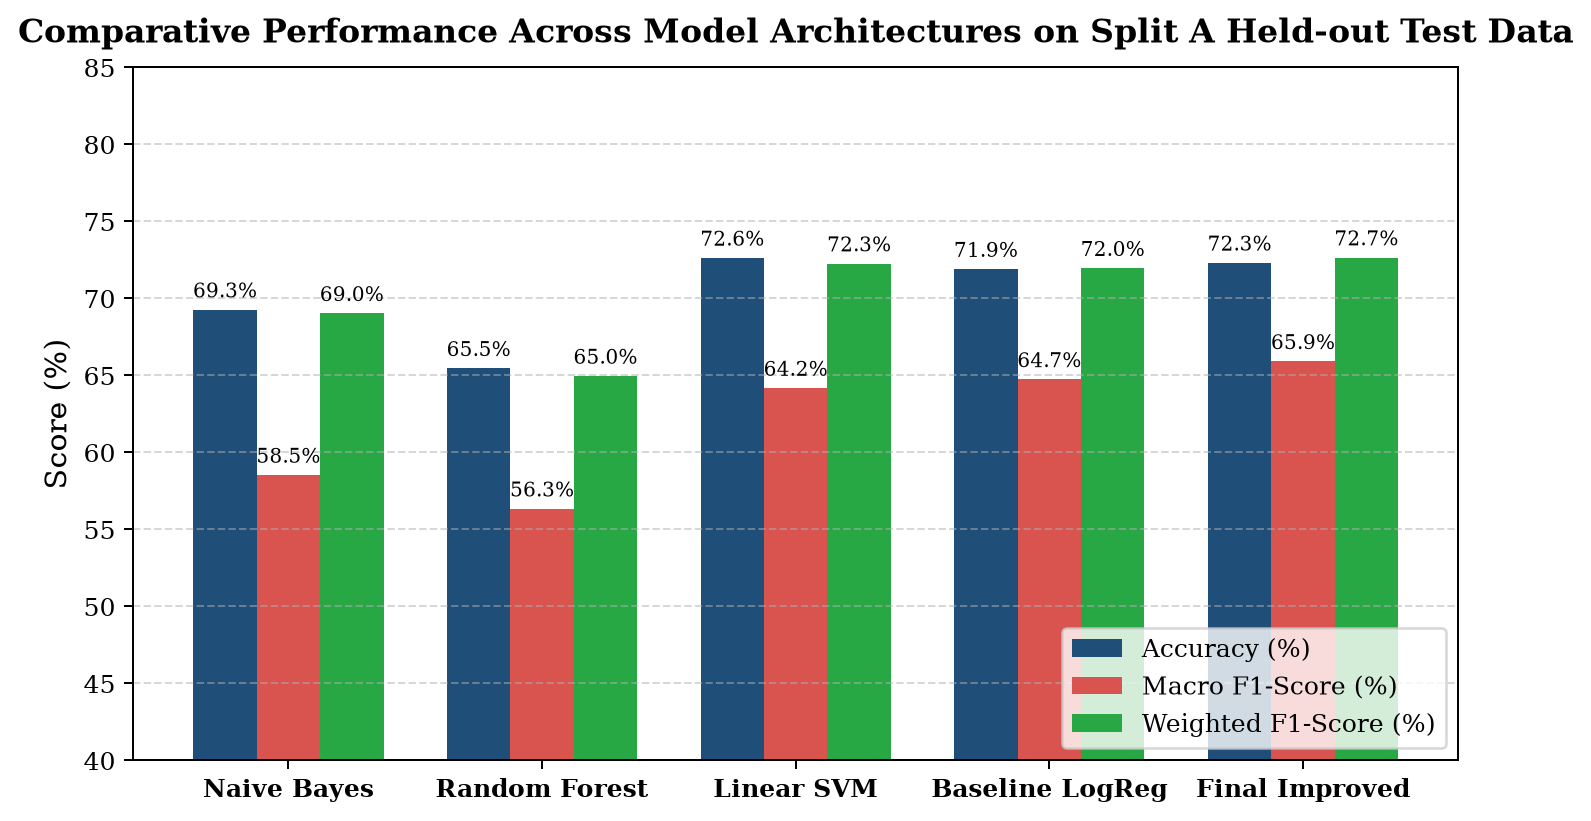
\includegraphics[width=0.88\textwidth]{figures/model_comparison_barchart.png}
\caption{Performance comparison of evaluated machine learning classifiers on held-out test data}\label{fig:model_comparison_barchart}
\end{figure}

\section{Evaluation metrics}
\label{sec:evaluation_metrics}

Evaluating multi-class classification on an imbalanced 41-category corpus requires a multi-faceted set of metrics. Let $C_k$ denote class $k$, and let $TP_k, FP_k, FN_k, TN_k$ represent True Positives, False Positives, False Negatives, and True Negatives for class $k$.

\begin{enumerate}
    \item Classification accuracy: The proportion of total test clauses correctly classified across all categories:
    \begin{equation}
        \text{Accuracy} = \frac{\sum_{k=0}^{K-1} TP_k}{N_{\text{test}}}
        \label{eq:accuracy}
    \end{equation}
    
    \item Macro-averaged precision, recall, and F1-score: Calculates the unweighted arithmetic mean across all $K = 41$ classes, treating rare and frequent categories equally:
    \begin{equation}
        \text{Macro-Precision} = \frac{1}{K} \sum_{k=0}^{K-1} \frac{TP_k}{TP_k + FP_k}, \quad
        \text{Macro-Recall} = \frac{1}{K} \sum_{k=0}^{K-1} \frac{TP_k}{TP_k + FN_k}
        \label{eq:macro_pr}
    \end{equation}
    \begin{equation}
        \text{Macro-F1} = \frac{1}{K} \sum_{k=0}^{K-1} \frac{2 \times \text{Precision}_k \times \text{Recall}_k}{\text{Precision}_k + \text{Recall}_k}
        \label{eq:macro_f1}
    \end{equation}

    \item Weighted-averaged F1-score: Weights each class's F1-score by its empirical test support $N_k$:
    \begin{equation}
        \text{Weighted-F1} = \sum_{k=0}^{K-1} \frac{N_k}{N_{\text{test}}} \text{F1}_k
        \label{eq:weighted_f1}
    \end{equation}

    \item Expected Calibration Error (ECE): Quantifies the divergence between predicted model confidence and actual empirical accuracy across $M = 10$ equally spaced confidence bins $B_m \subset (0, 1]$~\cite{guo2017calibration}:
    \begin{equation}
        \text{ECE} = \sum_{m=1}^{M} \frac{|B_m|}{N_{\text{test}}} \big|\text{acc}(B_m) - \text{conf}(B_m)\big|
        \label{eq:ece}
    \end{equation}
    where $\text{acc}(B_m) = \frac{1}{|B_m|} \sum_{i \in B_m} \mathbf{1}(\hat{y}_i = y_i)$ and $\text{conf}(B_m) = \frac{1}{|B_m|} \sum_{i \in B_m} \hat{p}_i$.
\end{enumerate}

\paragraph*{Confidence band analysis and reliability diagram}
Figure~\ref{fig:calibration_curve} presents the reliability diagram contrasting the baseline Logistic Regression model against the final improved model. The baseline model exhibited severe under-confidence in lower probability bins (clauses predicted with 25\% confidence actually attained $\sim$70\% accuracy), caused by 41 competing classes dispersing softmax probability mass. The final improved model achieves much tighter alignment with the ideal diagonal, reducing ECE to \FinalSplitAECE{}.

\begin{figure}[htbp]
\centering
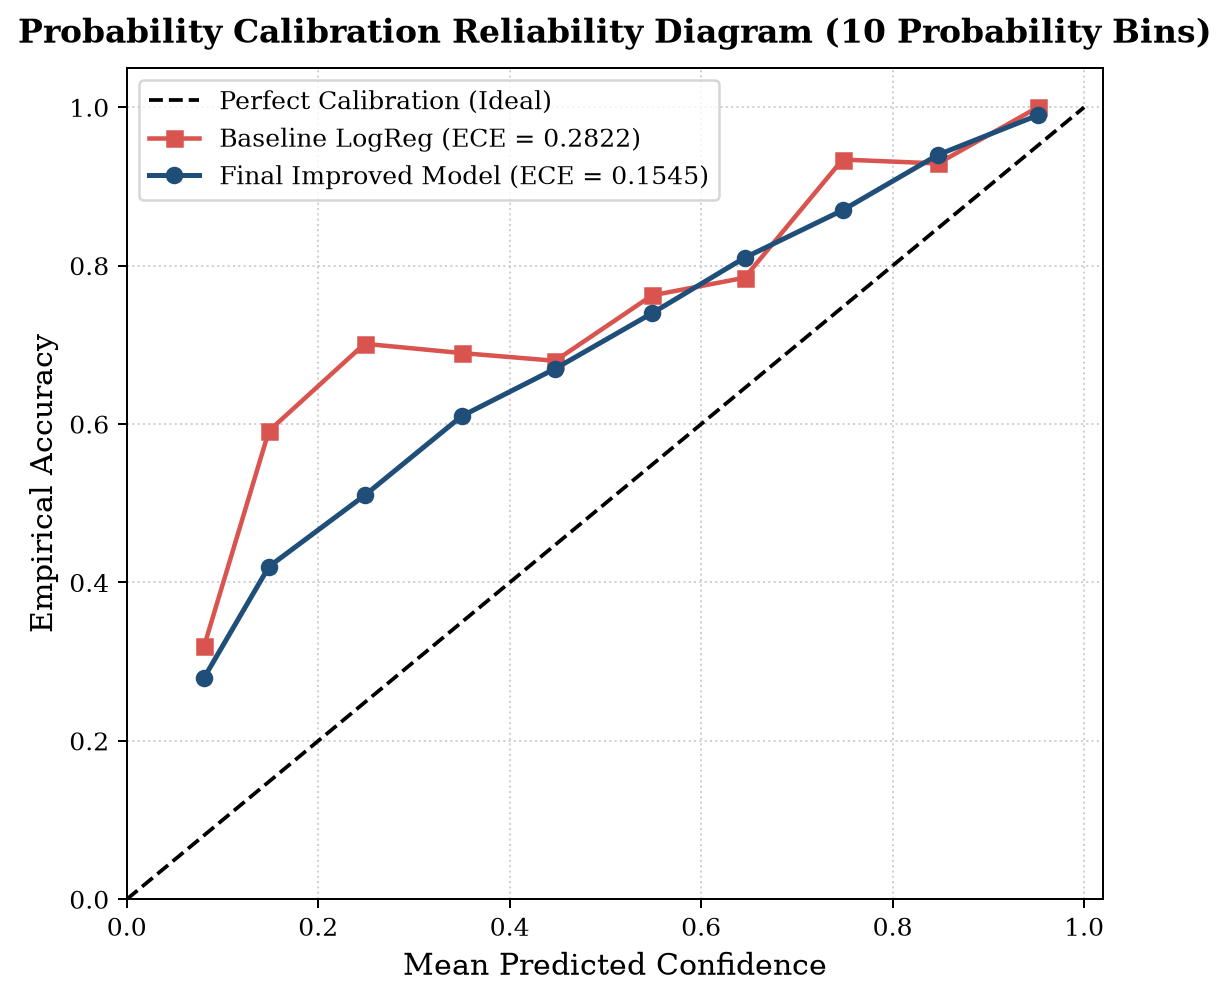
\includegraphics[width=0.75\textwidth]{figures/calibration_curve.png}
\caption{Reliability diagram comparing predicted confidence vs empirical accuracy across 10 probability bins}\label{fig:calibration_curve}
\end{figure}

Table~\ref{tab:confidence_tiers} details the empirical precision and sample coverage across operational confidence tiers on Split~B.

\begin{table}[htbp]
\centering
\footnotesize
\setlength{\tabcolsep}{5pt}
\begin{tabular}{lcccc}
\toprule
\textbf{Confidence Tier} & \textbf{Probability Rule} & \textbf{Clause Count} & \textbf{Corpus Share (\%)} & \textbf{Empirical Precision} \\
\midrule
High Confidence & $\hat{p} \ge 0.50$ & 1,323 & \FinalSplitBHighConfShare{} & \FinalSplitBHighConfPrec{} \\
Moderate Confidence & $0.25 \le \hat{p} < 0.50$ & 710 & 28.56\% & 66.90\% \\
Low Confidence -- Review & $0.10 \le \hat{p} < 0.25$ & 352 & 14.16\% & 50.38\% \\
Out of Scope & $\hat{p} < 0.10$ & 101 & 4.06\% & 28.30\% \\
\bottomrule
\end{tabular}
\caption{Operational confidence tier distribution and empirical precision (Split B, $N = 2,486$)}\label{tab:confidence_tiers}
\end{table}

Figure~\ref{fig:confidence_band_precision} plots empirical precision across confidence bins on both splits. Over 53\% of all predictions fall into the High Confidence tier, delivering an empirical precision of \FinalSplitBHighConfPrec{} on Split~B (and 81.95\% on Split~A). While this fell short of the initial ambitious 90\% precision target, it provides a trustworthy operational threshold: roughly 6 out of 7 High-confidence predictions are fully accurate, enabling legal teams to prioritize these clauses for accelerated sign-off while routing lower-confidence provisions to human reviewers.

\begin{figure}[htbp]
\centering
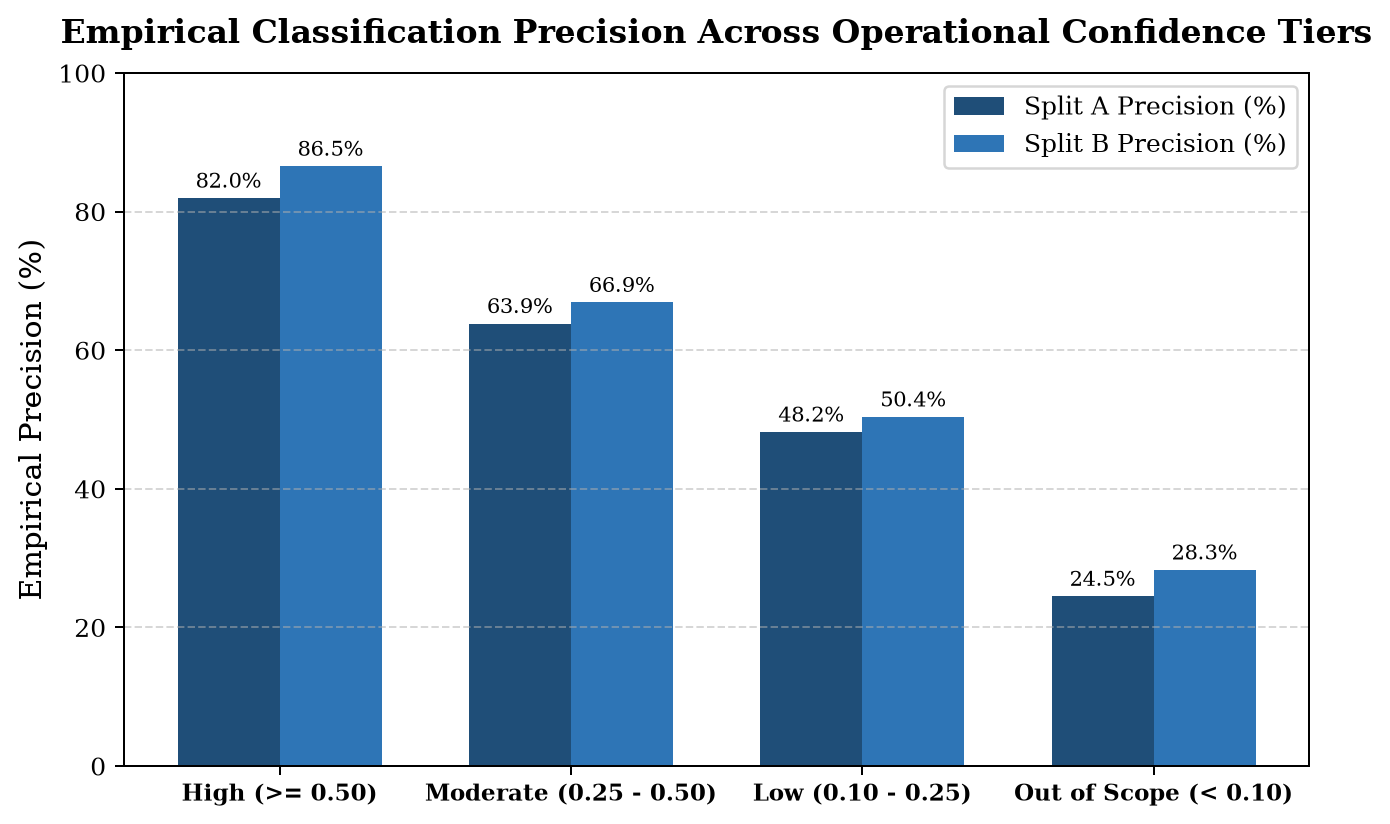
\includegraphics[width=0.82\textwidth]{figures/confidence_band_precision.png}
\caption{Empirical precision across operational confidence tiers on Split A and Split B}\label{fig:confidence_band_precision}
\end{figure}

\section{Confusion matrix}
\label{sec:confusion_matrix}

Figure~\ref{fig:confusion_matrix_split_a} displays the complete $41 \times 41$ multiclass confusion matrix for the final improved model evaluated on Split~A ($N = 2,441$).

\begin{figure}[htbp]
\centering
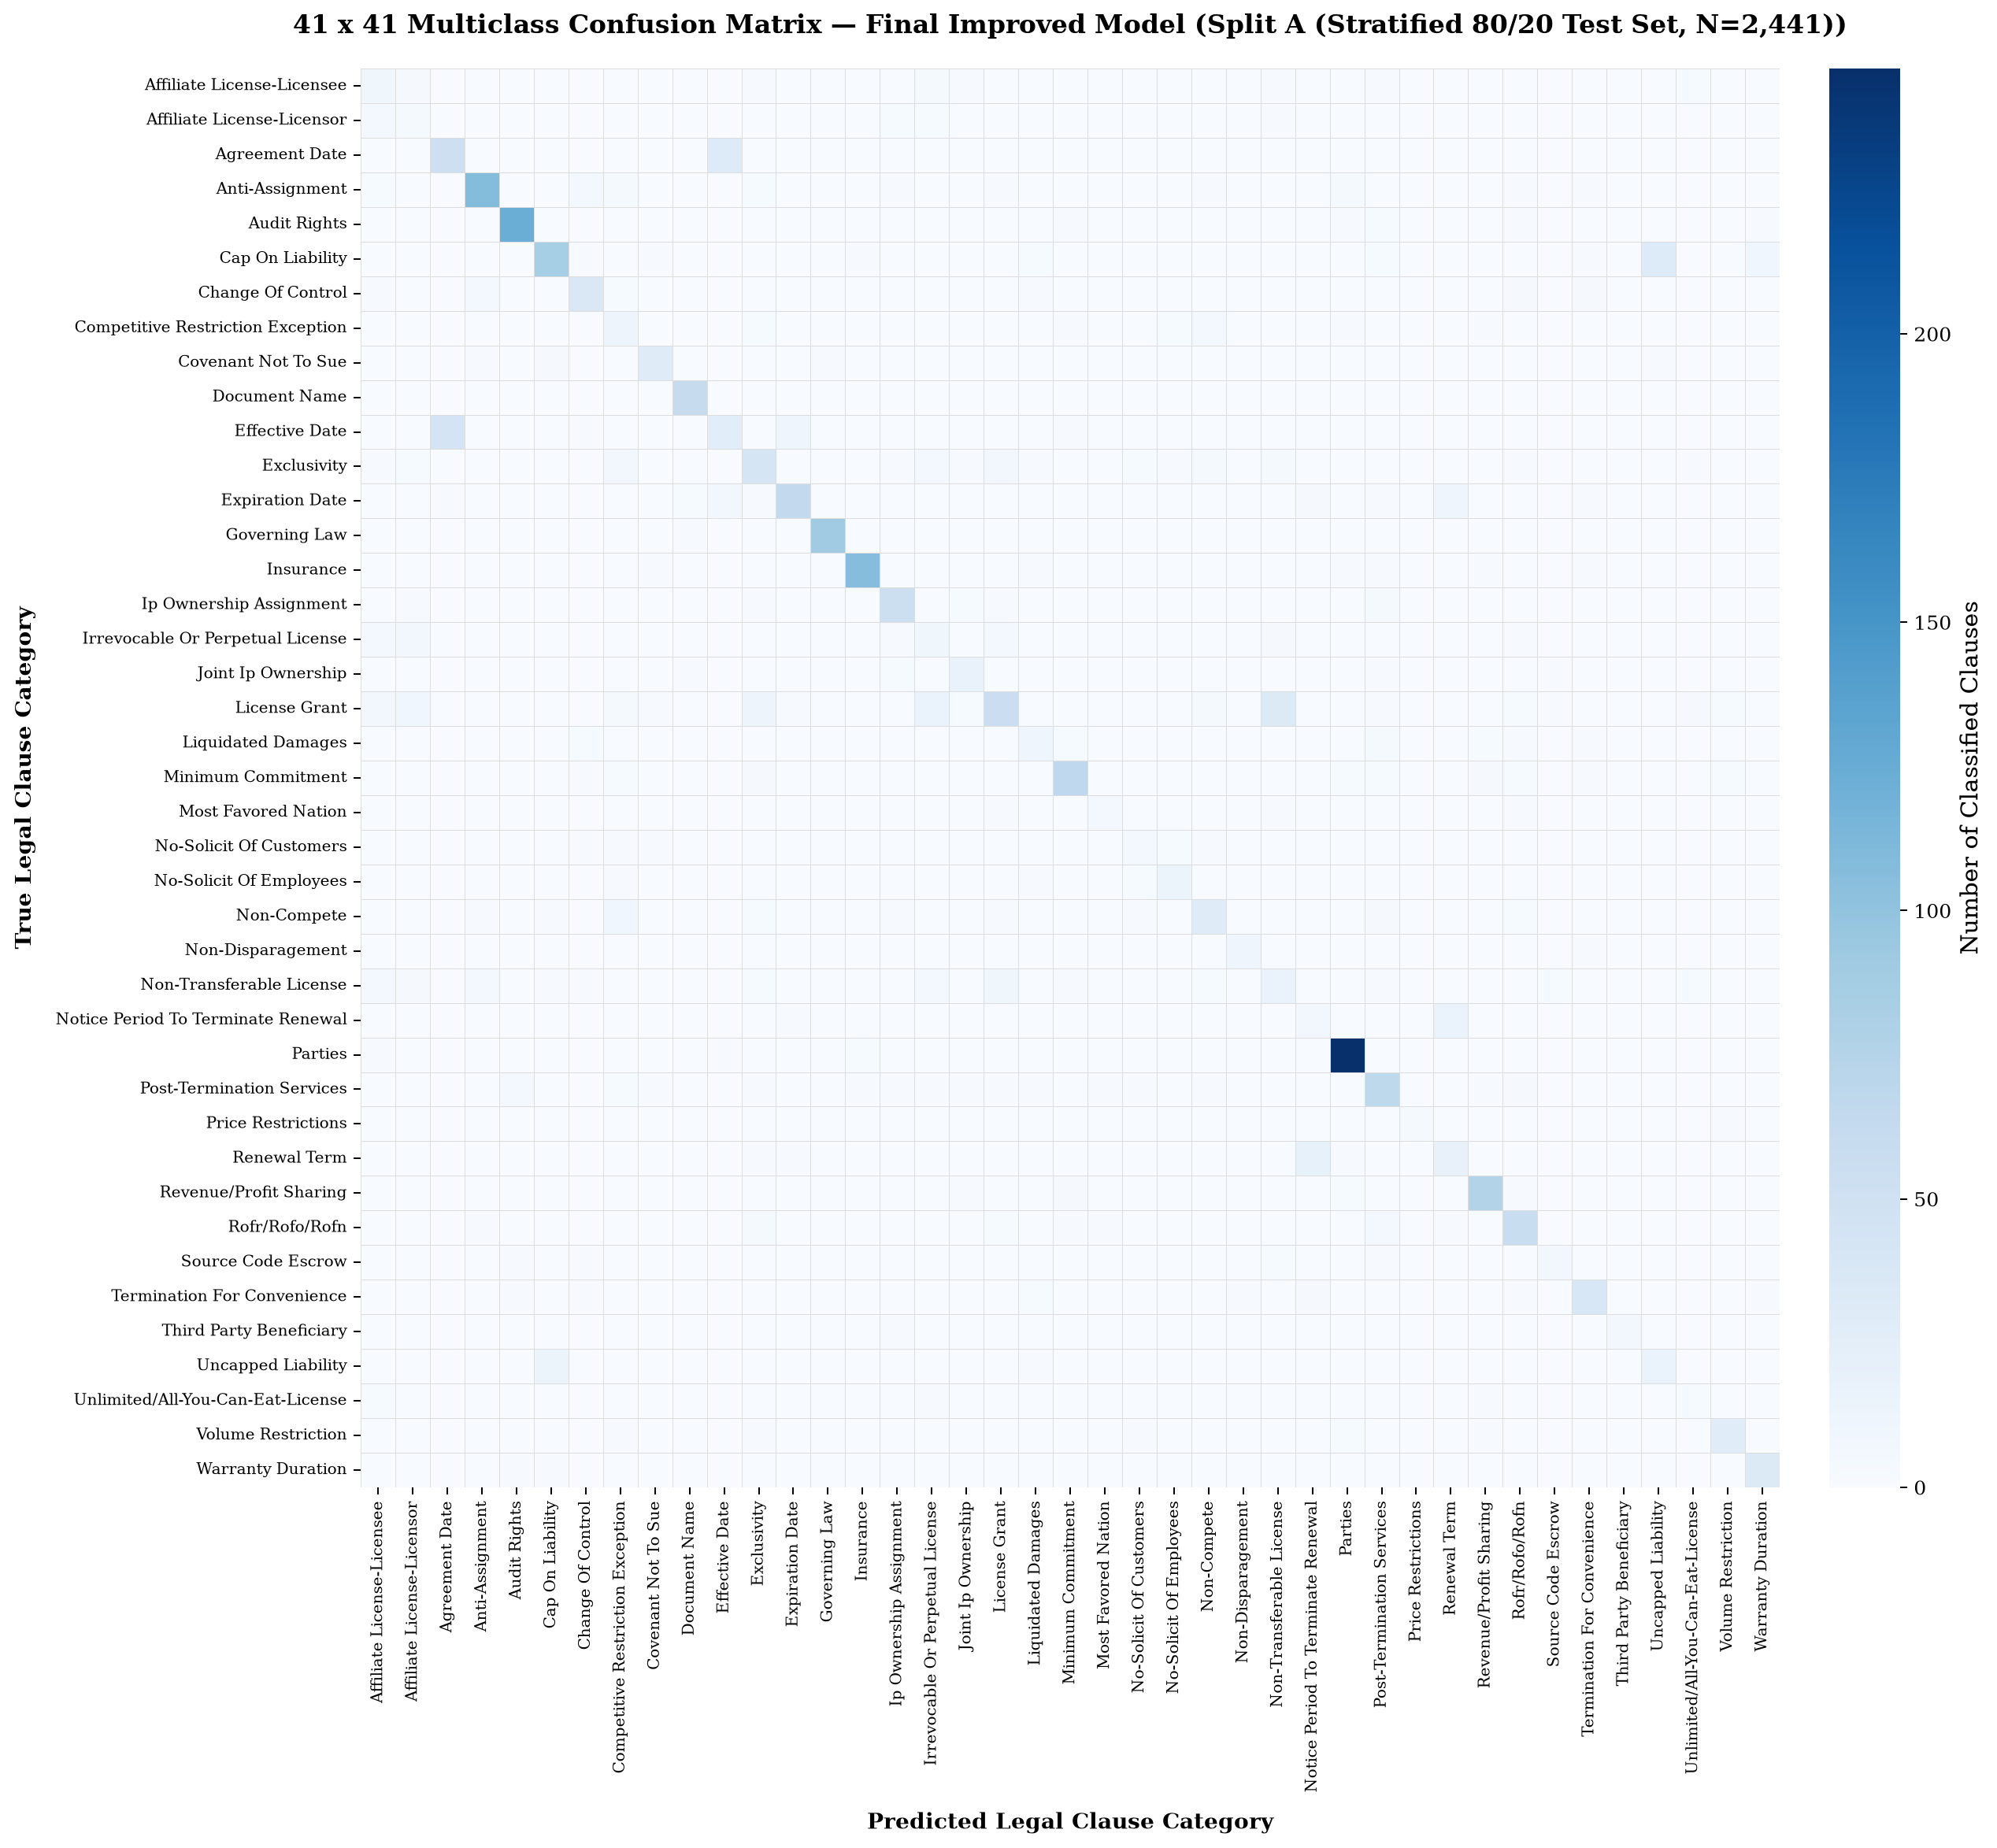
\includegraphics[width=0.98\textwidth]{figures/confusion_matrix_41x41_split_a.png}
\caption{Complete 41 $\times$ 41 confusion matrix on Split A ($N = 2,441$ held-out test clauses)}\label{fig:confusion_matrix_split_a}
\end{figure}

Figure~\ref{fig:confusion_matrix_split_b} displays the corresponding $41 \times 41$ confusion matrix evaluated on Split~B ($N = 2,486$ clauses across 102 unseen contracts). Both matrices exhibit heavy concentration along the main diagonal, confirming strong discriminative separation across distinct legal provisions.

\begin{figure}[htbp]
\centering
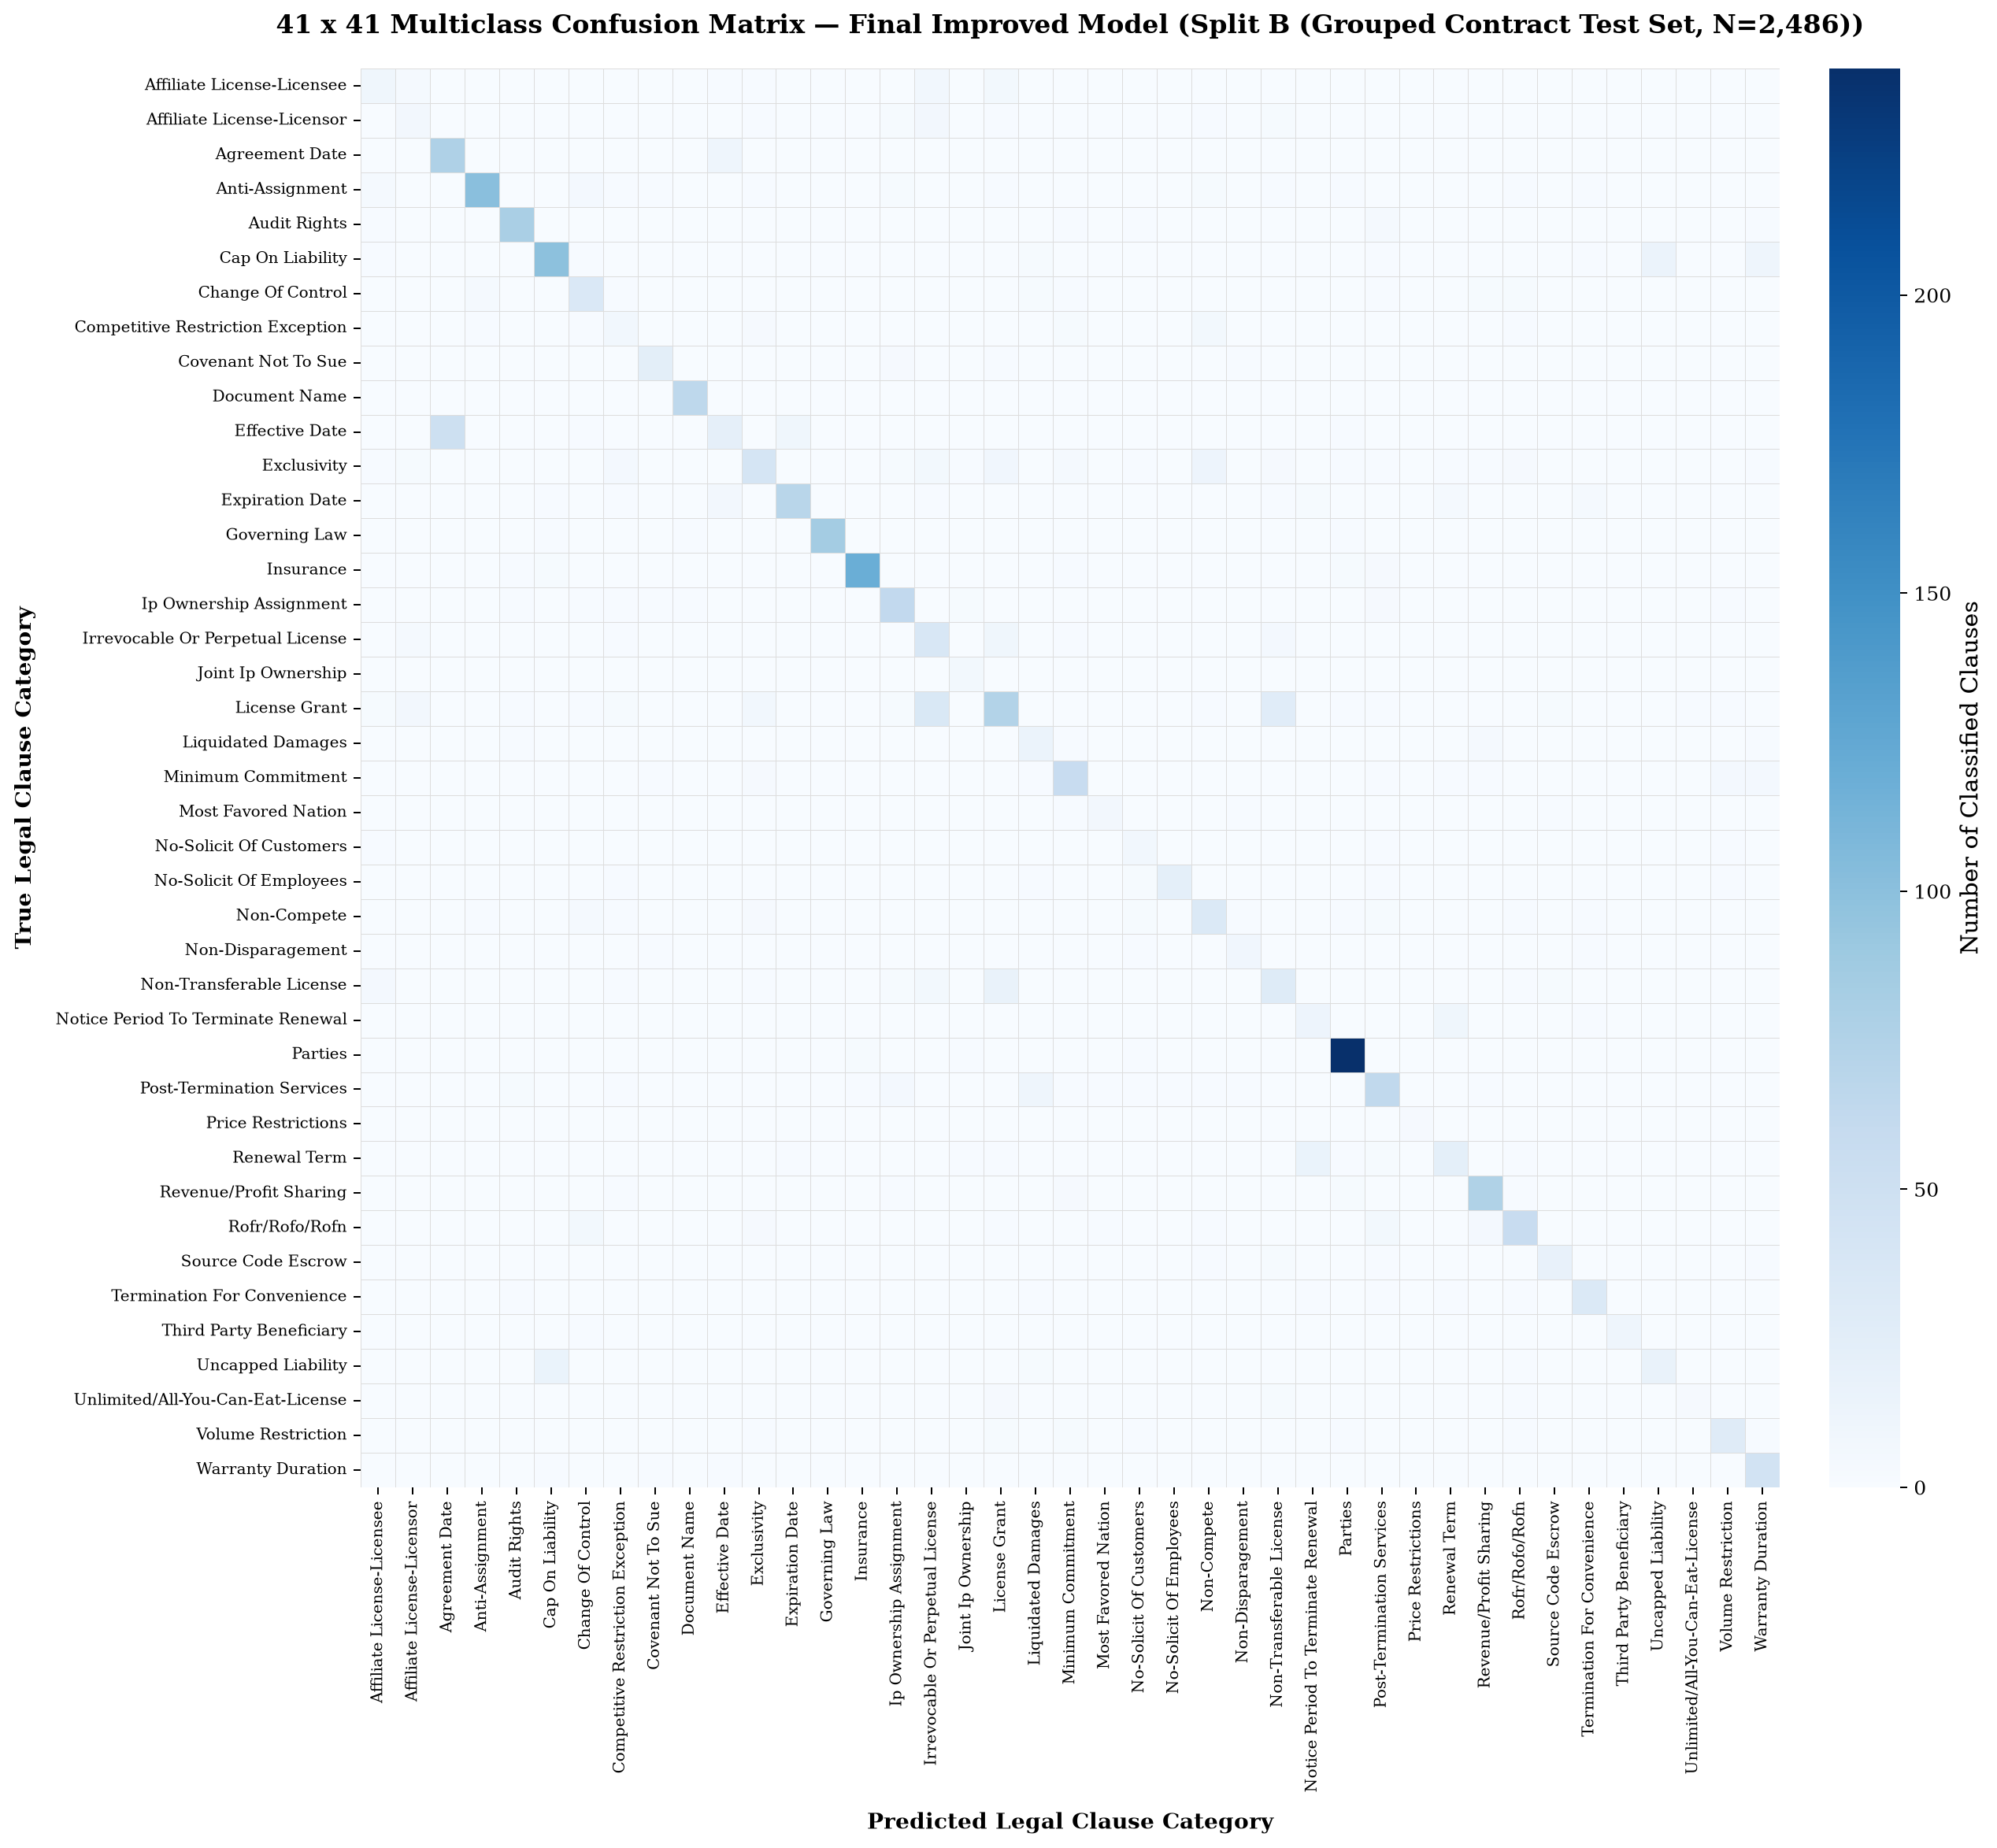
\includegraphics[width=0.98\textwidth]{figures/confusion_matrix_41x41_split_b.png}
\caption{Complete 41 $\times$ 41 confusion matrix on Split B ($N = 2,486$ grouped test clauses)}\label{fig:confusion_matrix_split_b}
\end{figure}

Figure~\ref{fig:per_class_f1_split_a_b} provides a comparative bar chart of per-class F1-scores across all 41 categories under Split~A and Split~B. Categories with distinctive statutory keywords (e.g., \textit{Governing Law}, \textit{Parties}, \textit{Audit Rights}) achieve F1-scores exceeding 0.90, whereas ambiguous licensing and notice categories experience greater variation.

\begin{figure}[htbp]
\centering
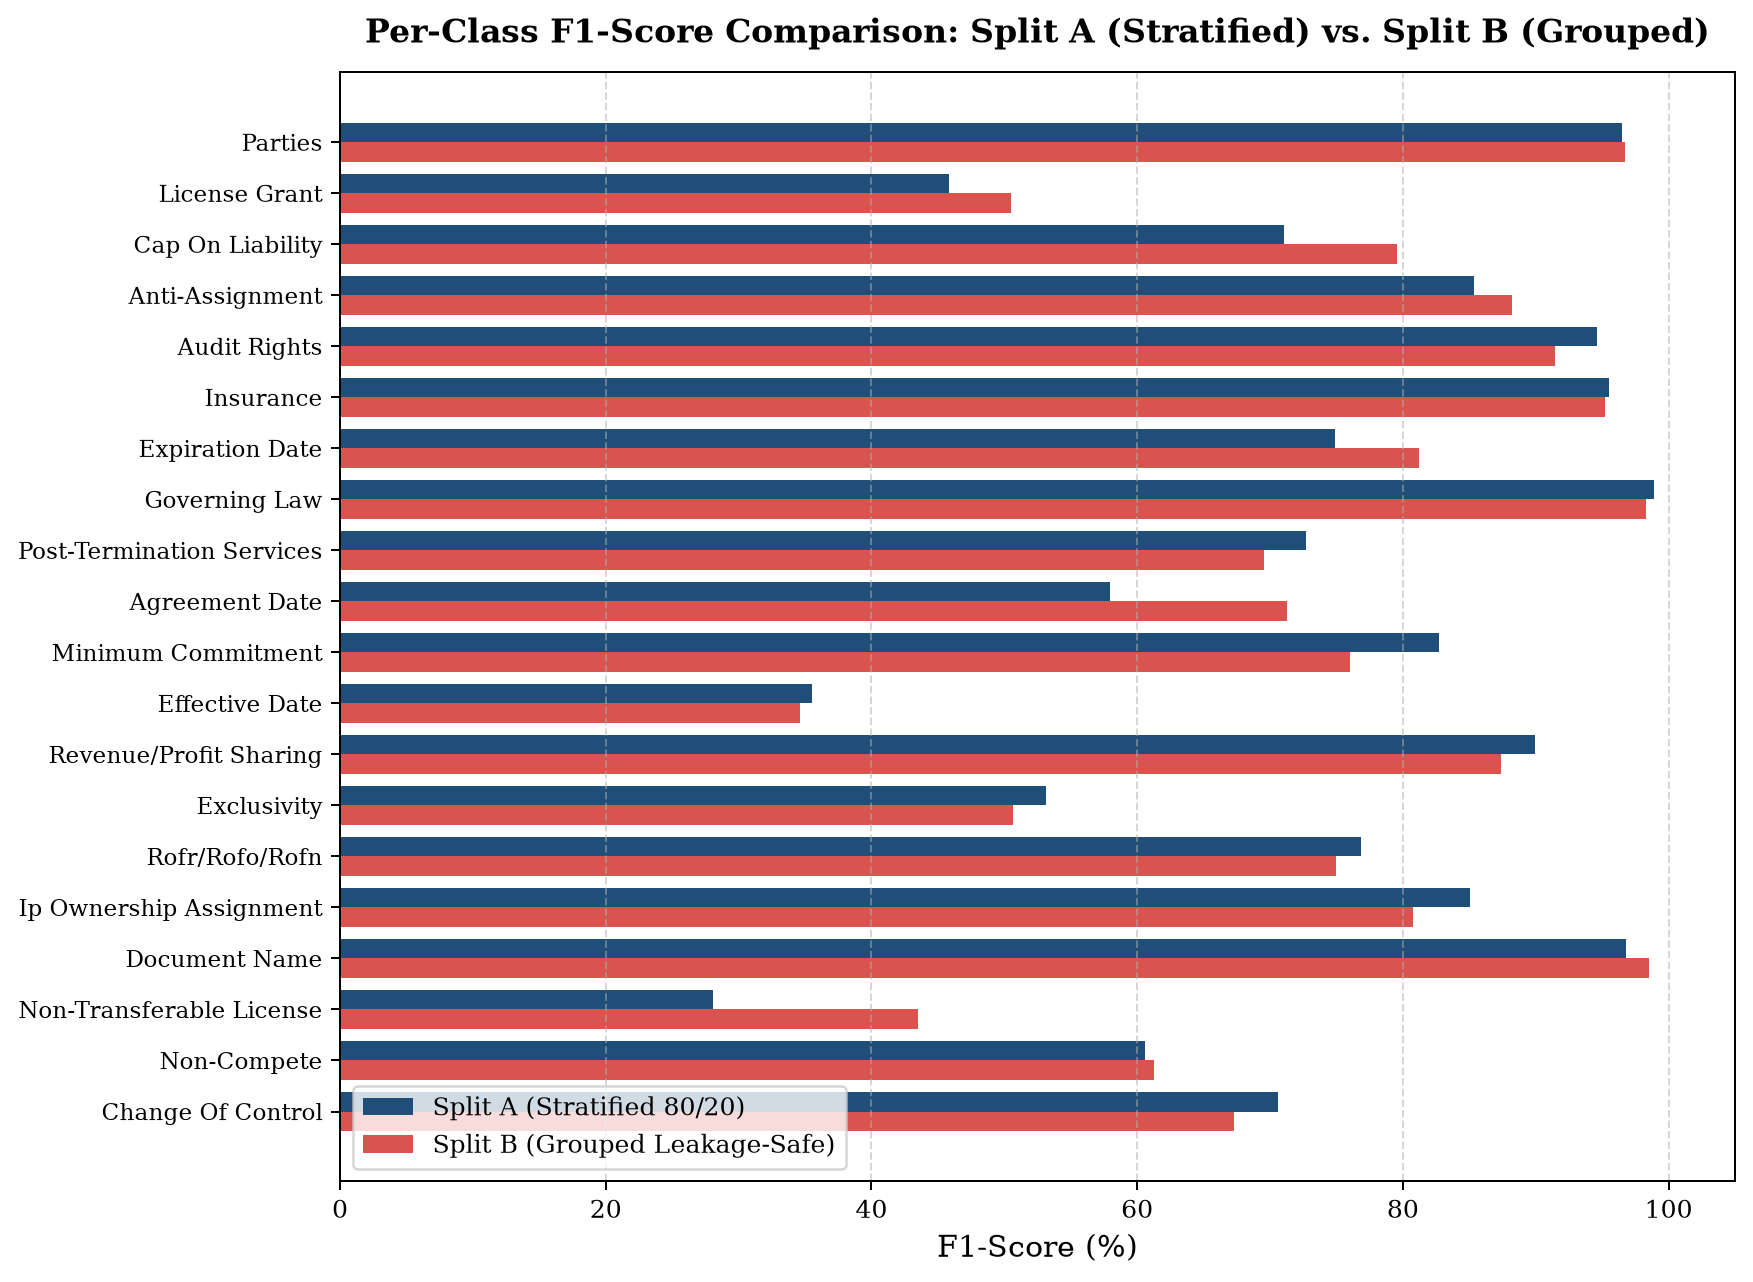
\includegraphics[width=0.95\textwidth]{figures/per_class_f1_split_a_b.png}
\caption{Per-class F1-scores across all 41 legal categories evaluated on Split A and Split B}\label{fig:per_class_f1_split_a_b}
\end{figure}

\paragraph*{Top confused category pairs analysis}
Table~\ref{tab:top_confused_pairs} reports the top systematically confused category pairs identified on Split~A, and Table~\ref{tab:top_confused_pairs_split_b} details the top confusions on Split~B. These table contents were arrived at by analyzing the off-diagonal cells of the $41 \times 41$ confusion matrix computed between ground-truth labels and model predictions. For every pair of categories $(i, j)$ where $i \neq j$, the count of instances where true class was $i$ but predicted class was $j$ was aggregated and sorted descending by frequency.

% Auto-generated by scripts/make_numbers.py
\begin{table}[htbp]
\centering
\footnotesize
\setlength{\tabcolsep}{3pt}
\begin{tabular}{r >{\raggedright\arraybackslash}p{3.0cm} >{\raggedright\arraybackslash}p{3.0cm} cc >{\raggedright\arraybackslash}p{5.2cm}}
\toprule
\textbf{\#} & \textbf{True Category} & \textbf{Predicted Category} & \textbf{Spl A} & \textbf{Spl B} & \textbf{Structural Root Cause} \\
\midrule
1 & Effective Date & Agreement Date & 44 & 51 & Shared temporal phrasing ('as of the date hereof', 'effective as of') \\
2 & License Grant & Non-Transferable License & 33 & 27 & Sub-licensing terms embedded in general grant paragraphs \\
3 & Cap On Liability & Uncapped Liability & 32 & 14 & Carve-outs inside limitation sections mentioning uncapped exceptions \\
4 & Agreement Date & Effective Date & 23 & 11 & Reciprocal confusion of date preamble clauses \\
5 & Renewal Term & Notice Period To Terminate Renewal & 20 & 15 & Renewal terms intertwined with termination notice deadlines \\
6 & License Grant & Irrevocable Or Perpetual License & 17 & 36 & Sub-licensing terms embedded in general grant paragraphs \\
7 & Notice Period To Terminate Renewal & Renewal Term & 16 & 10 & Renewal terms intertwined with termination notice deadlines \\
8 & Uncapped Liability & Cap On Liability & 15 & 15 & Carve-outs inside limitation sections mentioning uncapped exceptions \\
9 & License Grant & Exclusivity & 13 & 8 & High lexical overlap in commercial licensing rights \\
10 & Expiration Date & Renewal Term & 12 & 11 & Clauses specifying expiration alongside automatic renewal mechanics \\
11 & Effective Date & Expiration Date & 11 & 10 & Temporal date references in agreement period definitions \\
12 & Non-Transferable License & License Grant & 10 & 17 & Sub-licensing terms embedded in general grant paragraphs \\
\bottomrule
\end{tabular}
\caption{Top systematically confused category pairs identified in held-out test predictions}\label{tab:top_confused_pairs}
\end{table}


% Auto-generated by scripts/make_numbers.py
\begin{table}[htbp]
\centering
\footnotesize
\setlength{\tabcolsep}{3pt}
\begin{tabular}{r >{\raggedright\arraybackslash}p{3.2cm} >{\raggedright\arraybackslash}p{3.2cm} c >{\raggedright\arraybackslash}p{5.8cm}}
\toprule
\textbf{\#} & \textbf{True Category} & \textbf{Predicted Category} & \textbf{Count} & \textbf{Structural Root Cause} \\
\midrule
1 & Effective Date & Agreement Date & 51 & Shared temporal phrasing ('as of the date hereof', 'effective as of') \\
2 & License Grant & Irrevocable Or Perpetual License & 36 & Grant paragraphs containing duration qualifiers ('perpetual, irrevocable') \\
3 & License Grant & Non-Transferable License & 27 & Sub-licensing restrictions embedded within general grant language \\
4 & Renewal Term & Notice Period To Terminate Renewal & 15 & Renewal provisions conjoined with termination notice deadlines \\
5 & Uncapped Liability & Cap On Liability & 15 & Carve-out paragraphs stating uncapped exceptions inside limitation sections \\
6 & Cap On Liability & Uncapped Liability & 14 & Standard limitation provisions referencing liability caps and exceptions \\
7 & Agreement Date & Effective Date & 11 & Reciprocal preamble date mentions \\
8 & Expiration Date & Renewal Term & 11 & Fixed expiration statements intertwined with automatic renewal extensions \\
9 & Effective Date & Expiration Date & 10 & Temporal term definitions referencing start and end dates in adjacent sentences \\
10 & Notice Period To Terminate Renewal & Renewal Term & 10 & Reciprocal confusion regarding renewal timeline notices \\
\bottomrule
\end{tabular}
\caption{Top systematically confused category pairs on Split B (Grouped Contract-Held-out Partition)}\label{tab:top_confused_pairs_split_b}
\end{table}


Figure~\ref{fig:top_confused_pairs} and Figure~\ref{fig:top_confused_pairs_split_b} highlight the top misclassified pairs on both splits.

\begin{figure}[htbp]
\centering
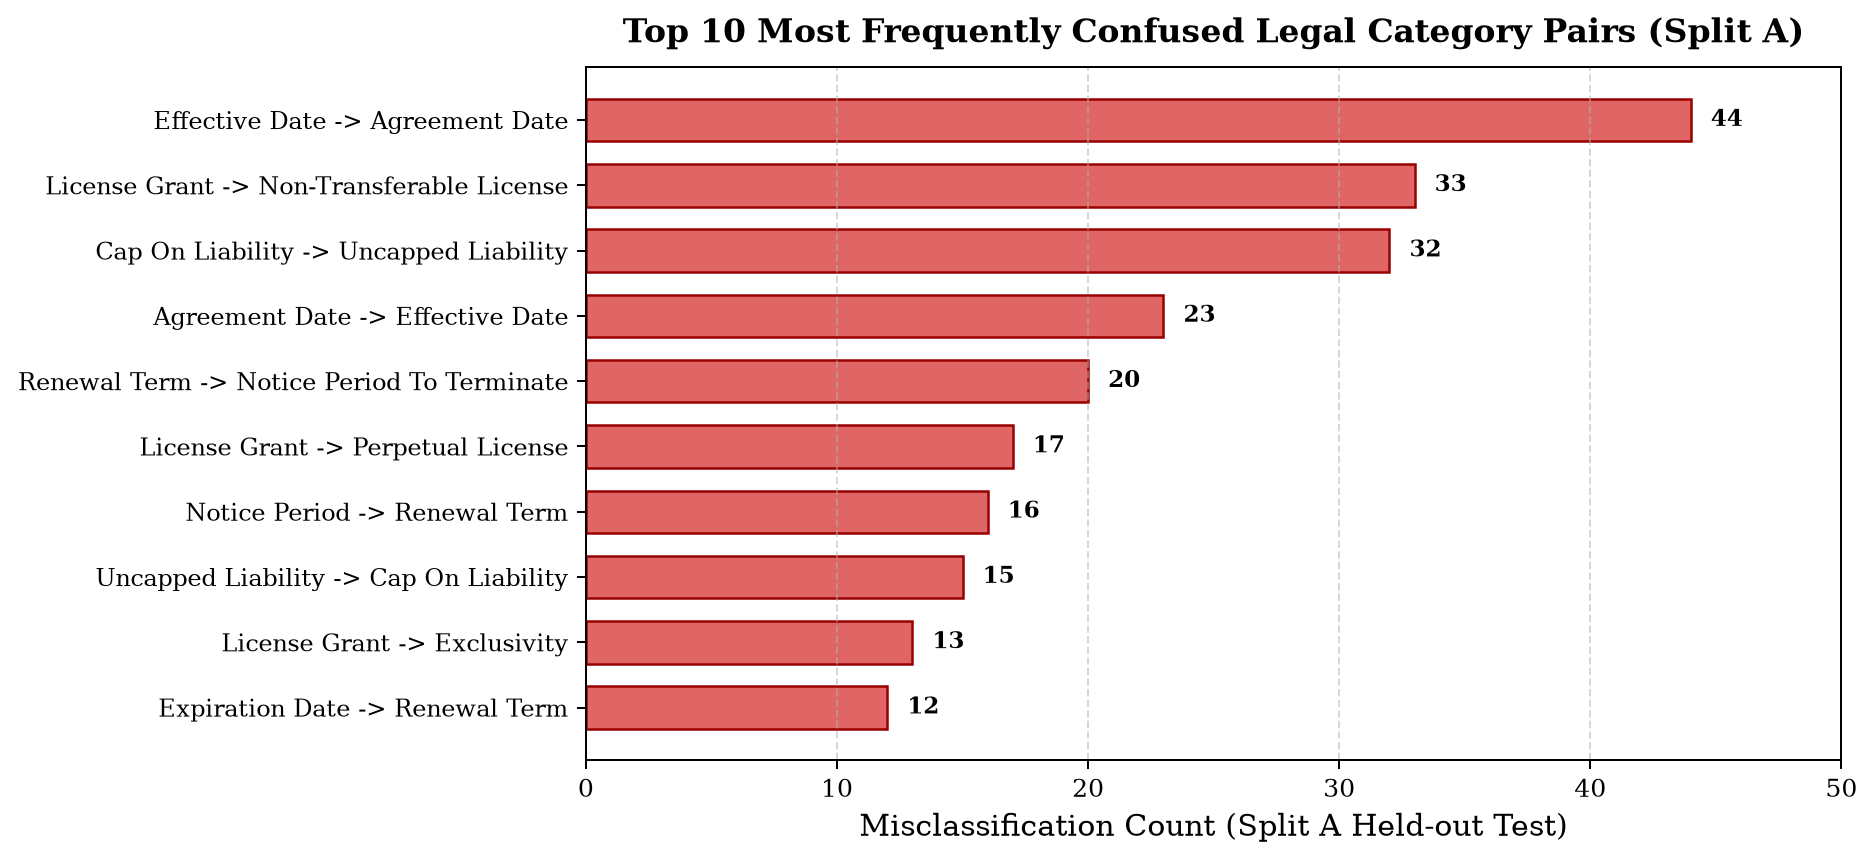
\includegraphics[width=0.82\textwidth]{figures/top_confused_pairs.png}
\caption{Top 10 most frequently confused legal category pairs on held-out test data (Split A)}\label{fig:top_confused_pairs}
\end{figure}

\begin{figure}[htbp]
\centering
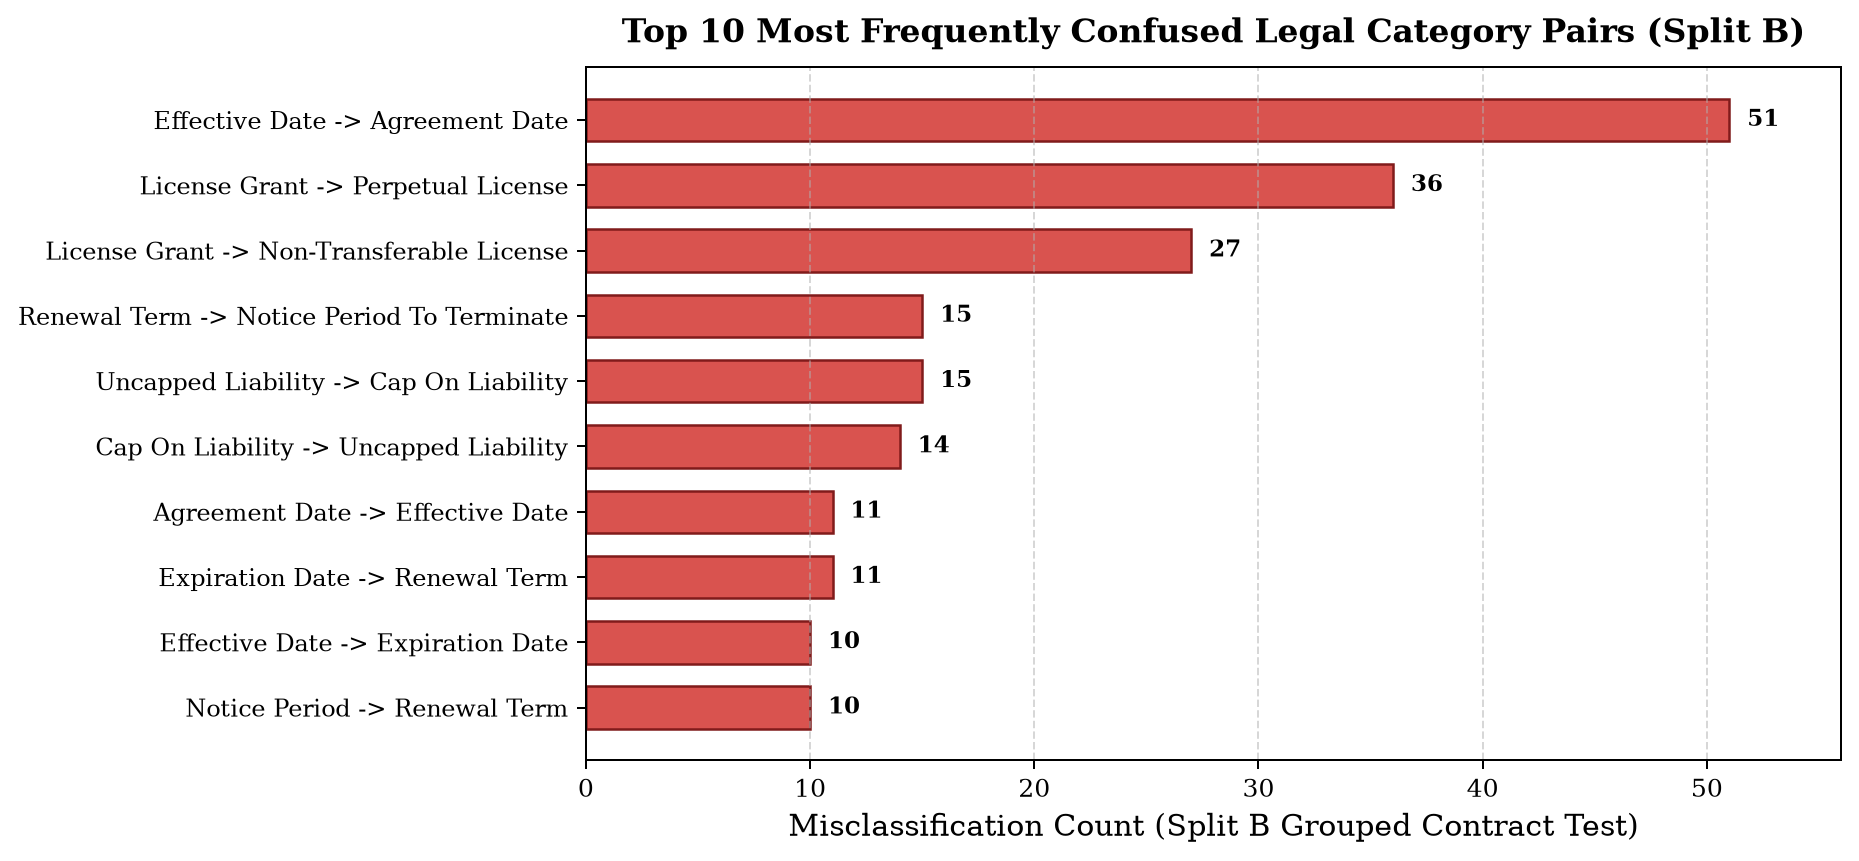
\includegraphics[width=0.82\textwidth]{figures/top_confused_pairs_split_b.png}
\caption{Top 10 most frequently confused legal category pairs on grouped test contracts (Split B)}\label{fig:top_confused_pairs_split_b}
\end{figure}

Inspection of real misclassified clauses from \texttt{docs/ERROR\_ANALYSIS.md} reveals the exact root causes of confusion:
\begin{enumerate}
    \item Effective Date vs Agreement Date (44 errors on Split A, 51 on Split B): Shared introductory recitals frequently bundle both dates into a single sentence. For example, a contract preamble states: \textit{``This Agreement is made and entered into as of January 15, 2020 by and between parties, and shall become effective as of February 1, 2020.''} Because both temporal markers co-occur, n-gram vectorizers without positional parsing assign probability mass to both labels.
    \item License Grant vs Non-Transferable License (33 errors on Split A, 27 on Split B): Intellectual property provisions routinely merge grant clauses with transfer restrictions: \textit{``Subject to the terms and conditions of this Agreement, NTL hereby grants to Entrust a non-transferable, non-assignable, indivisible, non-exclusive license.''} The clause is labeled \textit{Affiliate License-Licensor} in CUAD ground truth, but predicted as \textit{Non-Transferable License} (confidence 0.47) due to explicit restrictive modifiers.
    \item Cap On Liability vs Uncapped Liability (32 errors on Split A, 14 on Split B): Limitation of liability sections typically stipulate an aggregate monetary cap followed immediately by statutory exceptions: \textit{``Except for breaches of confidentiality, gross negligence, or willful misconduct, neither party's liability shall exceed the fees paid.''} The presence of both the cap rule and the uncapped carve-outs causes reciprocal confusion.
\end{enumerate}

\section{Relevant metrics calculated from the confusion matrix}
\label{sec:metrics_from_cm}

To provide an exhaustive diagnostic assessment, Table~\ref{tab:per_class_split_a} and Table~\ref{tab:per_class_split_b} report the exact per-class confusion counts (True Positives, False Positives, False Negatives, True Negatives) alongside Precision, Recall, Specificity, and F1-Score for all \NumClasses{} categories.

% Auto-generated by scripts/make_numbers.py
\begin{longtable}{>{\raggedright\arraybackslash}p{4.2cm} r r r r r r r r r}
\toprule
\textbf{Legal Category} & \textbf{Supp} & \textbf{TP} & \textbf{FP} & \textbf{FN} & \textbf{TN} & \textbf{Prec} & \textbf{Rec} & \textbf{Spec} & \textbf{F1} \\
\midrule
\endfirsthead
\multicolumn{10}{c}{{\bfseries Table \thetable\ continued from previous page}} \\
\toprule
\textbf{Legal Category} & \textbf{Supp} & \textbf{TP} & \textbf{FP} & \textbf{FN} & \textbf{TN} & \textbf{Prec} & \textbf{Rec} & \textbf{Spec} & \textbf{F1} \\
\midrule
\endhead
\midrule
\multicolumn{10}{r}{{Continued on next page}} \\
\bottomrule
\endfoot
\bottomrule
\caption{Comprehensive per-class classification metrics calculated from the 41$\times$41 confusion matrix on Split A (Stratified 80/20 held-out test, $N=2,441$)}\label{tab:per_class_split_a}\\
\endlastfoot
Affiliate License-Licensee & 23 & 10 & 30 & 13 & 2388 & 0.250 & 0.435 & 0.988 & 0.317 \\
Affiliate License-Licensor & 14 & 4 & 25 & 10 & 2402 & 0.138 & 0.286 & 0.990 & 0.186 \\
Agreement Date & 85 & 53 & 45 & 32 & 2311 & 0.541 & 0.624 & 0.981 & 0.579 \\
Anti-Assignment & 131 & 108 & 14 & 23 & 2296 & 0.885 & 0.824 & 0.994 & 0.854 \\
Audit Rights & 129 & 123 & 8 & 6 & 2304 & 0.939 & 0.953 & 0.997 & 0.946 \\
Cap On Liability & 135 & 86 & 21 & 49 & 2285 & 0.804 & 0.637 & 0.991 & 0.711 \\
Change Of Control & 51 & 36 & 15 & 15 & 2375 & 0.706 & 0.706 & 0.994 & 0.706 \\
Competitive Restriction Exception & 25 & 13 & 34 & 12 & 2382 & 0.277 & 0.520 & 0.986 & 0.361 \\
Covenant Not To Sue & 35 & 29 & 5 & 6 & 2401 & 0.853 & 0.829 & 0.998 & 0.841 \\
Document Name & 61 & 61 & 4 & 0 & 2376 & 0.938 & 1.000 & 0.998 & 0.968 \\
Effective Date & 84 & 27 & 41 & 57 & 2316 & 0.397 & 0.321 & 0.983 & 0.355 \\
Exclusivity & 82 & 42 & 34 & 40 & 2325 & 0.553 & 0.512 & 0.986 & 0.532 \\
Expiration Date & 93 & 64 & 14 & 29 & 2334 & 0.821 & 0.688 & 0.994 & 0.749 \\
Governing Law & 92 & 91 & 1 & 1 & 2348 & 0.989 & 0.989 & 1.000 & 0.989 \\
Insurance & 112 & 106 & 4 & 6 & 2325 & 0.964 & 0.946 & 0.998 & 0.955 \\
Ip Ownership Assignment & 63 & 54 & 10 & 9 & 2368 & 0.844 & 0.857 & 0.996 & 0.850 \\
Irrevocable Or Perpetual License & 33 & 10 & 36 & 23 & 2372 & 0.217 & 0.303 & 0.985 & 0.253 \\
Joint Ip Ownership & 23 & 18 & 8 & 5 & 2410 & 0.692 & 0.783 & 0.997 & 0.735 \\
License Grant & 155 & 55 & 30 & 100 & 2256 & 0.647 & 0.355 & 0.987 & 0.458 \\
Liquidated Damages & 24 & 12 & 10 & 12 & 2407 & 0.545 & 0.500 & 0.996 & 0.522 \\
Minimum Commitment & 85 & 67 & 10 & 18 & 2346 & 0.870 & 0.788 & 0.996 & 0.827 \\
Most Favored Nation & 8 & 5 & 2 & 3 & 2431 & 0.714 & 0.625 & 0.999 & 0.667 \\
No-Solicit Of Customers & 12 & 6 & 7 & 6 & 2422 & 0.462 & 0.500 & 0.997 & 0.480 \\
No-Solicit Of Employees & 18 & 14 & 5 & 4 & 2418 & 0.737 & 0.778 & 0.998 & 0.757 \\
Non-Compete & 51 & 30 & 18 & 21 & 2372 & 0.625 & 0.588 & 0.992 & 0.606 \\
Non-Disparagement & 13 & 12 & 1 & 1 & 2427 & 0.923 & 0.923 & 1.000 & 0.923 \\
Non-Transferable License & 59 & 17 & 45 & 42 & 2337 & 0.274 & 0.288 & 0.981 & 0.281 \\
Notice Period To Terminate Renewal & 24 & 7 & 26 & 17 & 2391 & 0.212 & 0.292 & 0.989 & 0.246 \\
Parties & 250 & 246 & 14 & 4 & 2177 & 0.946 & 0.984 & 0.994 & 0.965 \\
Post-Termination Services & 90 & 68 & 29 & 22 & 2322 & 0.701 & 0.756 & 0.988 & 0.727 \\
Price Restrictions & 5 & 4 & 0 & 1 & 2436 & 1.000 & 0.800 & 1.000 & 0.889 \\
Renewal Term & 42 & 19 & 29 & 23 & 2370 & 0.396 & 0.452 & 0.988 & 0.422 \\
Revenue/Profit Sharing & 83 & 76 & 10 & 7 & 2348 & 0.884 & 0.916 & 0.996 & 0.899 \\
Rofr/Rofo/Rofn & 73 & 58 & 20 & 15 & 2348 & 0.744 & 0.795 & 0.992 & 0.768 \\
Source Code Escrow & 13 & 8 & 4 & 5 & 2424 & 0.667 & 0.615 & 0.998 & 0.640 \\
Termination For Convenience & 49 & 39 & 10 & 10 & 2382 & 0.796 & 0.796 & 0.996 & 0.796 \\
Third Party Beneficiary & 8 & 7 & 0 & 1 & 2433 & 1.000 & 0.875 & 1.000 & 0.933 \\
Uncapped Liability & 33 & 17 & 33 & 16 & 2375 & 0.340 & 0.515 & 0.986 & 0.410 \\
Unlimited/All-You-Can-Eat-License & 6 & 2 & 8 & 4 & 2427 & 0.200 & 0.333 & 0.997 & 0.250 \\
Volume Restriction & 34 & 28 & 5 & 6 & 2402 & 0.848 & 0.824 & 0.998 & 0.836 \\
Warranty Duration & 35 & 33 & 11 & 2 & 2395 & 0.750 & 0.943 & 0.995 & 0.835 \\
\midrule
Macro Average & 2441 & - & - & - & - & 0.661 & 0.670 & 0.993 & 0.659 \\
Weighted Average & 2441 & - & - & - & - & 0.741 & 0.723 & 0.992 & 0.726 \\
\end{longtable}


\newpage
% Auto-generated by scripts/make_numbers.py
\begin{longtable}{>{\raggedright\arraybackslash}p{4.2cm} r r r r r r r r r}
\toprule
\textbf{Legal Category} & \textbf{Supp} & \textbf{TP} & \textbf{FP} & \textbf{FN} & \textbf{TN} & \textbf{Prec} & \textbf{Rec} & \textbf{Spec} & \textbf{F1} \\
\midrule
\endfirsthead
\multicolumn{10}{c}{{\bfseries Table \thetable\ continued from previous page}} \\
\toprule
\textbf{Legal Category} & \textbf{Supp} & \textbf{TP} & \textbf{FP} & \textbf{FN} & \textbf{TN} & \textbf{Prec} & \textbf{Rec} & \textbf{Spec} & \textbf{F1} \\
\midrule
\endhead
\midrule
\multicolumn{10}{r}{{Continued on next page}} \\
\bottomrule
\endfoot
\bottomrule
\caption{Comprehensive per-class classification metrics calculated from the 41$\times$41 confusion matrix on Split B (Grouped contract-held-out test, $N=2,486$)}\label{tab:per_class_split_b}\\
\endlastfoot
Affiliate License-Licensee & 30 & 10 & 15 & 20 & 2441 & 0.400 & 0.333 & 0.994 & 0.364 \\
Affiliate License-Licensor & 21 & 7 & 17 & 14 & 2448 & 0.292 & 0.333 & 0.993 & 0.311 \\
Agreement Date & 88 & 77 & 51 & 11 & 2347 & 0.602 & 0.875 & 0.979 & 0.713 \\
Anti-Assignment & 122 & 101 & 6 & 21 & 2358 & 0.944 & 0.828 & 0.997 & 0.882 \\
Audit Rights & 88 & 80 & 7 & 8 & 2391 & 0.920 & 0.909 & 0.997 & 0.914 \\
Cap On Liability & 130 & 99 & 20 & 31 & 2336 & 0.832 & 0.762 & 0.992 & 0.795 \\
Change Of Control & 48 & 35 & 21 & 13 & 2417 & 0.625 & 0.729 & 0.991 & 0.673 \\
Competitive Restriction Exception & 22 & 8 & 17 & 14 & 2447 & 0.320 & 0.364 & 0.993 & 0.340 \\
Covenant Not To Sue & 30 & 25 & 5 & 5 & 2451 & 0.833 & 0.833 & 0.998 & 0.833 \\
Document Name & 66 & 66 & 2 & 0 & 2418 & 0.971 & 1.000 & 0.999 & 0.985 \\
Effective Date & 85 & 22 & 20 & 63 & 2381 & 0.524 & 0.259 & 0.992 & 0.346 \\
Exclusivity & 96 & 41 & 25 & 55 & 2365 & 0.621 & 0.427 & 0.990 & 0.506 \\
Expiration Date & 90 & 69 & 11 & 21 & 2385 & 0.863 & 0.767 & 0.995 & 0.812 \\
Governing Law & 88 & 85 & 0 & 3 & 2398 & 1.000 & 0.966 & 1.000 & 0.983 \\
Insurance & 128 & 119 & 3 & 9 & 2355 & 0.975 & 0.930 & 0.999 & 0.952 \\
Ip Ownership Assignment & 74 & 63 & 19 & 11 & 2393 & 0.768 & 0.851 & 0.992 & 0.808 \\
Irrevocable Or Perpetual License & 59 & 38 & 64 & 21 & 2363 & 0.373 & 0.644 & 0.974 & 0.472 \\
Joint Ip Ownership & 6 & 6 & 5 & 0 & 2475 & 0.545 & 1.000 & 0.998 & 0.706 \\
License Grant & 167 & 74 & 52 & 93 & 2267 & 0.587 & 0.443 & 0.978 & 0.505 \\
Liquidated Damages & 21 & 14 & 20 & 7 & 2445 & 0.412 & 0.667 & 0.992 & 0.509 \\
Minimum Commitment & 75 & 57 & 18 & 18 & 2393 & 0.760 & 0.760 & 0.993 & 0.760 \\
Most Favored Nation & 10 & 7 & 2 & 3 & 2474 & 0.778 & 0.700 & 0.999 & 0.737 \\
No-Solicit Of Customers & 11 & 8 & 10 & 3 & 2465 & 0.444 & 0.727 & 0.996 & 0.552 \\
No-Solicit Of Employees & 29 & 23 & 1 & 6 & 2456 & 0.958 & 0.793 & 1.000 & 0.868 \\
Non-Compete & 51 & 34 & 26 & 17 & 2409 & 0.567 & 0.667 & 0.989 & 0.613 \\
Non-Disparagement & 12 & 9 & 4 & 3 & 2470 & 0.692 & 0.750 & 0.998 & 0.720 \\
Non-Transferable License & 65 & 30 & 43 & 35 & 2378 & 0.411 & 0.462 & 0.982 & 0.435 \\
Notice Period To Terminate Renewal & 24 & 13 & 18 & 11 & 2444 & 0.419 & 0.542 & 0.993 & 0.473 \\
Parties & 242 & 238 & 12 & 4 & 2232 & 0.952 & 0.983 & 0.995 & 0.967 \\
Post-Termination Services & 91 & 64 & 29 & 27 & 2366 & 0.688 & 0.703 & 0.988 & 0.696 \\
Price Restrictions & 3 & 3 & 0 & 0 & 2483 & 1.000 & 1.000 & 1.000 & 1.000 \\
Renewal Term & 45 & 23 & 17 & 22 & 2424 & 0.575 & 0.511 & 0.993 & 0.541 \\
Revenue/Profit Sharing & 84 & 76 & 14 & 8 & 2388 & 0.844 & 0.905 & 0.994 & 0.874 \\
Rofr/Rofo/Rofn & 80 & 57 & 15 & 23 & 2391 & 0.792 & 0.713 & 0.994 & 0.750 \\
Source Code Escrow & 23 & 18 & 5 & 5 & 2458 & 0.783 & 0.783 & 0.998 & 0.783 \\
Termination For Convenience & 40 & 34 & 9 & 6 & 2437 & 0.791 & 0.850 & 0.996 & 0.819 \\
Third Party Beneficiary & 12 & 11 & 0 & 1 & 2474 & 1.000 & 0.917 & 1.000 & 0.957 \\
Uncapped Liability & 35 & 17 & 14 & 18 & 2437 & 0.548 & 0.486 & 0.994 & 0.515 \\
Unlimited/All-You-Can-Eat-License & 9 & 3 & 1 & 6 & 2476 & 0.750 & 0.333 & 1.000 & 0.462 \\
Volume Restriction & 38 & 29 & 9 & 9 & 2439 & 0.763 & 0.763 & 0.996 & 0.763 \\
Warranty Duration & 48 & 45 & 21 & 3 & 2417 & 0.682 & 0.938 & 0.991 & 0.789 \\
\midrule
Macro Average & 2486 & - & - & - & - & 0.698 & 0.712 & 0.993 & 0.695 \\
Weighted Average & 2486 & - & - & - & - & 0.749 & 0.739 & 0.992 & 0.737 \\
\end{longtable}


\paragraph*{Step-by-step worked mathematical examples}
To demonstrate the exact mathematical derivation of the diagnostic metrics from the confusion matrix, three representative classes---one high-frequency category (\textit{Governing Law}), one ambiguous borderline category (\textit{Cap On Liability}), and one rare low-support category (\textit{Affiliate License-Licensor})---are worked through step by step.

% Auto-generated by scripts/make_numbers.py
\begin{examplebox}{Worked Example 1: Governing Law (High-Performing Class)}
From the $41 \times 41$ confusion matrix on Split A ($N = 2,441$):
\begin{itemize}
\item True Positives ($TP$) = 91 (clauses correctly identified as Governing Law)
\item False Positives ($FP$) = 1 (other clause mistakenly predicted as Governing Law)
\item False Negatives ($FN$) = 1 (Governing Law clause mistakenly assigned to another class)
\item True Negatives ($TN$) = $2441 - (91 + 1 + 1) = 2348$ (non-Governing Law clauses correctly rejected)
\end{itemize}
Calculating the diagnostic metrics step by step:
\begin{align*}
\text{Precision} &= \frac{TP}{TP + FP} = \frac{91}{91 + 1} = \frac{91}{92} = 0.9891 \quad (98.91\%)\\
\text{Recall (Sensitivity)} &= \frac{TP}{TP + FN} = \frac{91}{91 + 1} = \frac{91}{92} = 0.9891 \quad (98.91\%)\\
\text{Specificity} &= \frac{TN}{TN + FP} = \frac{2348}{2348 + 1} = \frac{2348}{2349} = 0.9996 \quad (99.96\%)\\
\text{F1-Score} &= 2 \times \frac{\text{Precision} \times \text{Recall}}{\text{Precision} + \text{Recall}} = 2 \times \frac{0.9891 \times 0.9891}{0.9891 + 0.9891} = 0.9891 \quad (98.91\%)
\end{align*}
\end{examplebox}

\begin{examplebox}{Worked Example 2: Cap On Liability (Ambiguous Borderline Class)}
From the $41 \times 41$ confusion matrix on Split A ($N = 2,441$):
\begin{itemize}
\item True Positives ($TP$) = 86 (clauses correctly identified as Cap On Liability)
\item False Positives ($FP$) = 21 (non-cap clauses mistakenly predicted as Cap On Liability)
\item False Negatives ($FN$) = 49 (Cap On Liability clauses misclassified, e.g., as Uncapped Liability)
\item True Negatives ($TN$) = $2441 - (86 + 21 + 49) = 2285$ (clauses of all other 40 categories correctly rejected)
\end{itemize}
Step-by-step substitution into evaluation formulas:
\begin{align*}
\text{Precision} &= \frac{86}{86 + 21} = \frac{86}{107} = 0.8037 \quad (80.37\%)\\
\text{Recall} &= \frac{86}{86 + 49} = \frac{86}{135} = 0.6370 \quad (63.70\%)\\
\text{Specificity} &= \frac{2285}{2285 + 21} = \frac{2285}{2306} = 0.9909 \quad (99.09\%)\\
\text{F1-Score} &= 2 \times \frac{0.8037 \times 0.6370}{0.8037 + 0.6370} = 0.7107 \quad (71.07\%)
\end{align*}
\end{examplebox}

\begin{examplebox}{Worked Example 3: Affiliate License-Licensor (Low-Support Class)}
From the $41 \times 41$ confusion matrix on Split A ($N = 2,441$):
\begin{itemize}
\item True Positives ($TP$) = 4 (rare license clauses correctly predicted)
\item False Positives ($FP$) = 25 (other clauses mistakenly predicted as this category)
\item False Negatives ($FN$) = 10 (target clauses misassigned to License Grant or Non-Transferable License)
\item True Negatives ($TN$) = $2441 - (4 + 25 + 10) = 2402$ (all remaining corpus clauses correctly rejected)
\end{itemize}
Evaluation results for rare class:
\begin{align*}
\text{Precision} &= \frac{4}{4 + 25} = \frac{4}{29} = 0.1379 \quad (13.79\%)\\
\text{Recall} &= \frac{4}{4 + 10} = \frac{4}{14} = 0.2857 \quad (28.57\%)\\
\text{Specificity} &= \frac{2402}{2402 + 25} = \frac{2402}{2427} = 0.9897 \quad (98.97\%)\\
\text{F1-Score} &= 2 \times \frac{0.1379 \times 0.2857}{0.1379 + 0.2857} = 0.1860 \quad (18.60\%)
\end{align*}
\end{examplebox}


\section{Prediction statistics of unseen data}
\label{sec:unseen_data}

Model robustness was validated across four levels of unseen evaluation data:

\paragraph*{1. Held-out Split A test partition ($N = 2,441$)}
On the uniformly held-out 20\% test partition, the model classified 1,765 of 2,441 clauses correctly, achieving \FinalSplitAAcc{} Accuracy, \FinalSplitAMacroFScore{} Macro-F1, and \FinalSplitAWeightedFScore{} Weighted-F1. High-frequency categories with distinct legal vocabulary achieved high precision: \textit{Governing Law} reached F1 = 0.989 (98.9\%), \textit{Parties} achieved F1 = 0.965 (96.5\%), and \textit{Audit Rights} achieved F1 = 0.946 (94.6\%).

\paragraph*{2. Held-out Split B grouped contracts ($N = 2,486$)}
On the 102 completely held-out commercial agreements with zero training contract overlap, the model achieved \FinalSplitBAcc{} Accuracy, \FinalSplitBMacroFScore{} Macro-F1, and \FinalSplitBWeightedFScore{} Weighted-F1. The consistency between Split~A and Split~B indicates that the model generalizes across independent drafting styles.

\paragraph*{3. Real-document PDF extraction and classification}
The real-document ingestion pipeline (\path{api/services/ml_service.py}) was tested on local PDF agreements using PyMuPDF and the boundary tokenizer in \path{src/clause_splitter.py}:
\begin{enumerate}
    \item \path{data/raw_pdfs/sample_contract.pdf}: The clause splitter extracted exactly 29 discrete clauses. Table~\ref{tab:real_pdf_check} lists all 29 extracted clauses, reporting the text snippet, predicted legal category, operational confidence score, and triage status.
    \item \path{test_data/ClauseIQ_Synthetic_Company_Service_Agreement_Test.pdf}: The clause splitter extracted 69 discrete clauses, identifying provisions including \textit{Parties}, \textit{Expiration Date}, \textit{Renewal Term}, and \textit{Governing Law}.
\end{enumerate}

% Auto-generated by scripts/make_numbers.py
\begin{longtable}{r >{\raggedright\arraybackslash}p{6.8cm} >{\raggedright\arraybackslash}p{3.8cm} c >{\raggedright\arraybackslash}p{2.6cm}}
\toprule
\textbf{\#} & \textbf{Extracted Clause Text Snippet} & \textbf{Predicted Category} & \textbf{Conf} & \textbf{Assigned Tier} \\
\midrule
\endfirsthead
\multicolumn{5}{c}{{\bfseries Table \thetable\ continued from previous page}} \\
\toprule
\textbf{\#} & \textbf{Extracted Clause Text Snippet} & \textbf{Predicted Category} & \textbf{Conf} & \textbf{Assigned Tier} \\
\midrule
\endhead
\midrule
\multicolumn{5}{r}{{Continued on next page}} \\
\bottomrule
\endfoot
\bottomrule
\caption[Clause-level parsing and classification audit for unseen sample contract PDF]{Full clause-level parsing and classification audit for unseen \texttt{sample\_contract.pdf} (29 clauses extracted)}\label{tab:real_pdf_check}\\
\endlastfoot
1 & SAMPLE SERVICE AGREEMENT This Sample Service Agreement (the ``Agre\dots & Document Name & 61.8\% & High confidence \\
2 & Ltd.\dots & Parties & 88.8\% & High confidence \\
3 & (``Company'') and XYZ Solutions (``Service Provider'').\dots & Parties & 81.1\% & High confidence \\
4 & 1.\dots & Parties & 84.6\% & High confidence \\
5 & Confidentiality The Service Provider shall keep confidential all \dots & Audit Rights & 21.6\% & Low confidence – Review Required \\
6 & The Service Provider shall not disclose such information to any t\dots & Anti-Assignment & 54.5\% & High confidence \\
7 & 2.\dots & Parties & 84.5\% & High confidence \\
8 & Payment Terms The Company shall pay the Service Provider a total \dots & Revenue/Profit Sharing & 63.6\% & High confidence \\
9 & Invoices shall be submitted monthly and shall be paid within thir\dots & Warranty Duration & 12.3\% & Low confidence – Review Required \\
10 & 3.\dots & Parties & 84.7\% & High confidence \\
11 & Term and Termination This Agreement shall commence on January 15,\dots & Expiration Date & 67.4\% & High confidence \\
12 & Either party may terminate this Agreement by providing thirty (30\dots & Termination For Convenience & 72.8\% & High confidence \\
13 & Either party may terminate immediately in the event of a material\dots & Termination For Convenience & 39.8\% & Moderate confidence \\
14 & 4.\dots & Parties & 84.8\% & High confidence \\
15 & Intellectual Property All reports, documents, software, designs, \dots & Ip Ownership Assignment & 79.7\% & High confidence \\
16 & Pre-existing intellectual property of either party shall remain t\dots & Ip Ownership Assignment & 27.5\% & Moderate confidence \\
17 & 5.\dots & Parties & 84.5\% & High confidence \\
18 & Indemnification The Service Provider shall indemnify and hold har\dots & Cap On Liability & 66.5\% & High confidence \\
19 & 6.\dots & Parties & 84.8\% & High confidence \\
20 & Limitation of Liability Neither party shall be liable for indirec\dots & Cap On Liability & 74.9\% & High confidence \\
21 & The aggregate liability of either party under this Agreement shal\dots & Cap On Liability & 66.1\% & High confidence \\
22 & 7.\dots & Parties & 84.6\% & High confidence \\
23 & Governing Law This Agreement shall be governed by and construed i\dots & Governing Law & 89.7\% & High confidence \\
24 & The courts located in Bengaluru, Karnataka shall have exclusive j\dots & Governing Law & 37.1\% & Moderate confidence \\
25 & 8.\dots & Parties & 85.0\% & High confidence \\
26 & Notices All notices under this Agreement shall be made in writing\dots & Anti-Assignment & 9.5\% & Out of supported category scope \\
27 & For ABC Technologies Pvt.\dots & Parties & 83.5\% & High confidence \\
28 & Ltd.\dots & Parties & 88.8\% & High confidence \\
29 & For XYZ Solutions Authorized Signatory: \_\_\_\_\_\_\_\_\_\_\_\_\_\_\_\_\_\_\_\_ Auth\dots & Parties & 48.9\% & Moderate confidence \\
\end{longtable}


\textit{Methodological Note:} The real-PDF test corpus consists of two sample documents. While these tests verify that the PDF parsing, text extraction, clause splitting, and classification pipeline functions without runtime crashes or schema violations, two documents represent a tiny sample size that cannot support broad statistical conclusions. In the absence of exhaustive human gold-standard annotations for every extracted snippet, predictions are reported objectively without asserting definitive correctness.

\paragraph*{Intelligent search retrieval evaluation}
Table~\ref{tab:search_evaluation} documents the retrieval performance of the TF-IDF and Cosine Similarity intelligent search engine across five benchmark legal queries evaluated over the entire 12,204-clause corpus.

% Auto-generated by scripts/make_numbers.py
\begin{table}[htbp]
\centering
\footnotesize
\setlength{\tabcolsep}{3.5pt}
\begin{tabular}{>{\raggedright\arraybackslash}p{3.2cm} >{\raggedright\arraybackslash}p{3.5cm} ccccccc}
\toprule
\textbf{Query} & \textbf{Target Category} & \textbf{Corpus N} & \textbf{P@1} & \textbf{P@3} & \textbf{P@5} & \textbf{P@10} & \textbf{R@5} & \textbf{R@10} \\
\midrule
termination for convenience & Termination For Convenience & 246 & 1.00 & 0.67 & 0.60 & 0.70 & 0.0122 & 0.0285 \\
governing law & Governing Law & 462 & 1.00 & 1.00 & 1.00 & 0.90 & 0.0108 & 0.0195 \\
non-compete & Non-Compete & 257 & 0.00 & 0.67 & 0.80 & 0.90 & 0.0156 & 0.0350 \\
limitation of liability & Cap On Liability, Uncapped Liability & 839 & 1.00 & 1.00 & 1.00 & 0.90 & 0.0060 & 0.0107 \\
audit rights & Audit Rights & 642 & 1.00 & 1.00 & 1.00 & 0.90 & 0.0078 & 0.0140 \\
\bottomrule
\end{tabular}
\caption{Information retrieval evaluation for TF-IDF and Cosine Similarity search across benchmark legal queries}\label{tab:search_evaluation}
\end{table}


Figure~\ref{fig:search_metrics_p_at_k} illustrates the Precision@k retrieval curves across retrieval depths $k \in \{1, 3, 5, 10\}$. The horizontal axis represents the cutoff rank ($k$), defining the number of top-ranked clauses returned by the TF-IDF Cosine Similarity engine. The vertical axis measures Precision@k ($\text{P}@k = \frac{\text{Relevant Clauses in Top-}k}{k}$), denoting the proportion of retrieved provisions that strictly belong to the intended target legal category.

Each colored curve in Figure~\ref{fig:search_metrics_p_at_k} represents a distinct benchmark legal query evaluated against the 12,204-clause corpus:
\begin{itemize}
    \item Orange curve (\textit{Query: 'governing law...'}): Evaluates retrieval for jurisdictional choice-of-law covenants. It sustains a flat, perfect precision of 1.00 at $k=1, 3, 5$ and 0.90 at $k=10$. This consistent precision is driven by standardized, explicit jurisdictional phrasing (e.g., ``governed by and construed in accordance with the laws of the State of...'') that produces strong, isolated cosine similarity peaks.
    \item Red curve (\textit{Query: 'limitation of liability...'}): Evaluates liability caps and consequential damage disclaimers. It maintains 1.00 precision from $k=1$ through $k=5$ and 0.90 at $k=10$, reflecting the highly stereotyped vocabulary characteristic of commercial risk allocation provisions (e.g., ``in no event shall aggregate liability exceed'', ``indirect, special, or consequential damages'').
    \item Purple curve (\textit{Query: 'audit rights...'}): Evaluates inspection covenants. It achieves 1.00 precision across $k=1, 3, 5$ and 0.90 at $k=10$, reliably isolating books, records, and financial accounting examination provisions.
    \item Blue curve (\textit{Query: 'termination for convenience...'}): Evaluates discretionary termination rights. It starts with perfect precision of 1.00 at $k=1$, exhibits a slight dip to 0.67 at $k=3$ and 0.60 at $k=5$, and stabilizes at 0.70 at $k=10$. This dip occurs because general termination-for-cause and contract expiration clauses share substantial lexical overlap (e.g., ``terminate'', ``written notice'', ``effective date'') with convenience covenants, introducing false positives at intermediate ranks.
    \item Green curve (\textit{Query: 'non-compete...'}): Evaluates restrictive commercial covenants. It starts at 0.00 at $k=1$, then climbs steeply to 0.67 at $k=3$, 0.80 at $k=5$, and 0.90 at $k=10$. The initial $k=1$ score occurs because a closely related restrictive covenant (such as an Exclusivity or Non-Solicitation provision containing competitive restrictions) ranked first; however, as the retrieval window expands to $k \ge 3$, true Non-Compete provisions dominate the results.
\end{itemize}

Across all benchmark legal queries, the search engine delivers an average Precision@1 of 0.80 and Precision@5 of 0.88, demonstrating that the cosine retrieval engine reliably surfaces legally relevant provisions for open-ended practitioner queries.

\begin{figure}[htbp]
\centering
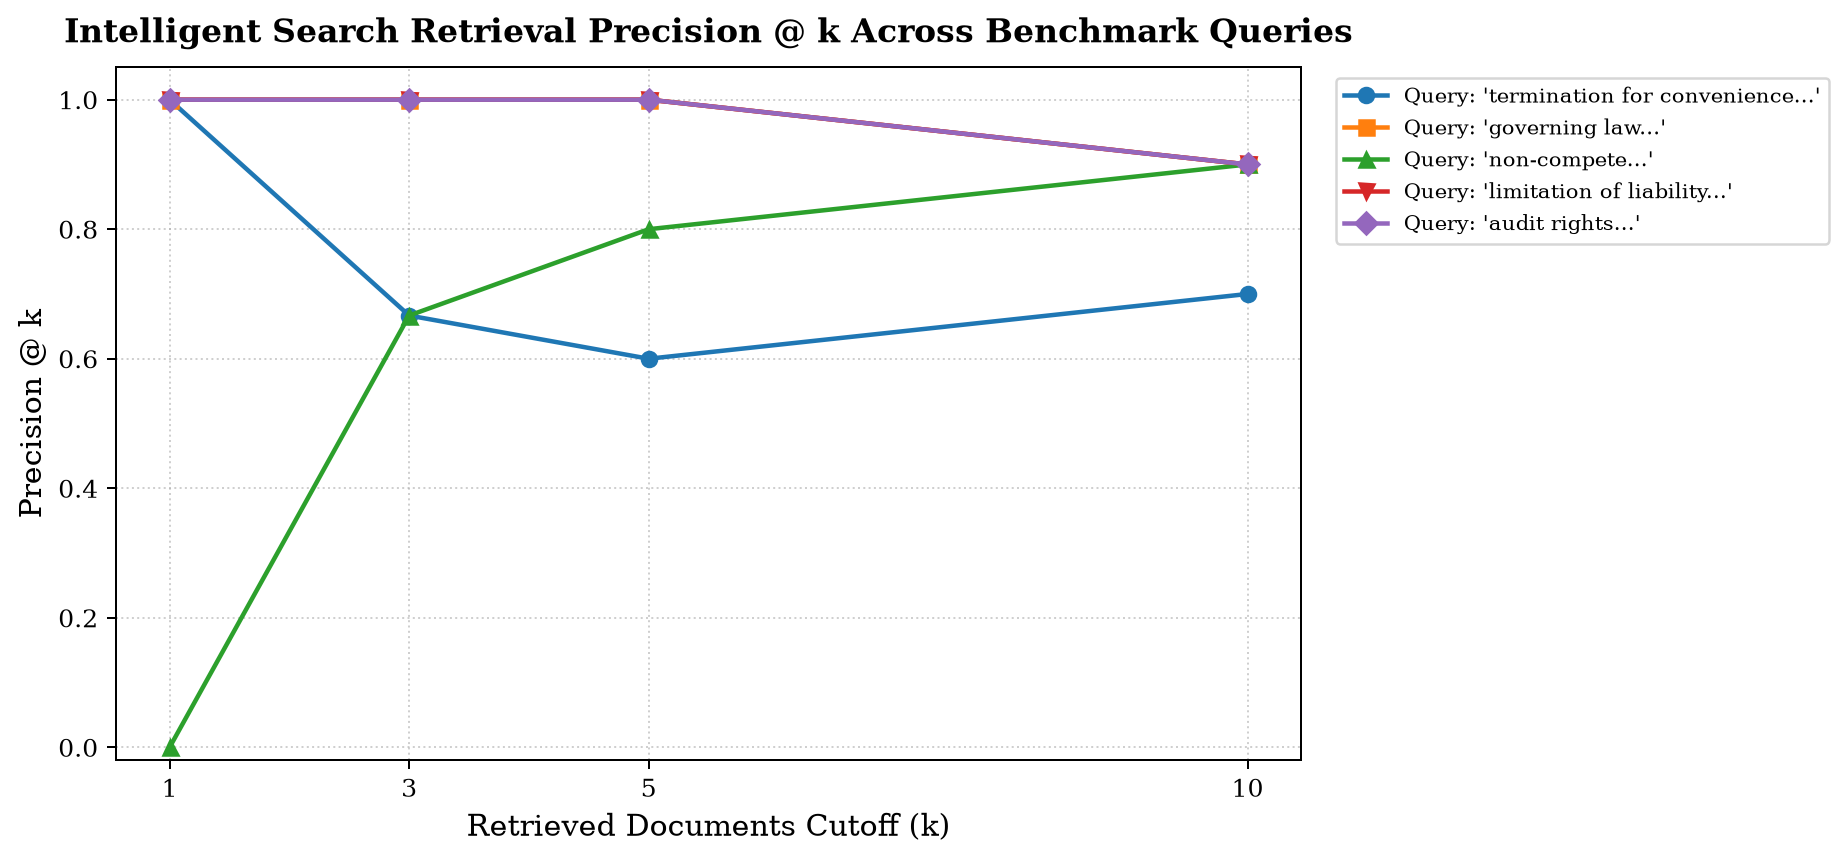
\includegraphics[width=0.82\textwidth]{figures/search_metrics_p_at_k.png}
\caption{Precision @ k retrieval performance across benchmark legal queries}\label{fig:search_metrics_p_at_k}
\end{figure}

\section{Discussion of findings and conclusions}
\label{sec:discussion_findings}

The empirical evaluation of ClauseIQ substantiates several critical findings:

\begin{enumerate}
    \item Efficacy of classical architectures: Multinomial Logistic Regression paired with a 40,000-feature hybrid word and character n-gram representation delivers 72.31\% accuracy and 65.91\% Macro-F1 across 41 imbalanced categories, outperforming Random Forest (64.36\%) and Naive Bayes (69.27\%) while matching Linear SVM (72.63\%) without sacrificing posterior probability outputs.
    \item Resilience across parent contracts: Benchmarking against Split~B (GroupShuffleSplit by contract) demonstrated that contract-level grouping does not cause catastrophic degradation (73.93\% accuracy, 69.47\% Macro-F1), indicating that the classifiers learned substantive covenant vocabulary rather than contract-specific party metadata.
    \item Mechanism of calibration improvement: In systematic experiments (EXP-05-SIG and EXP-05-ISO in \texttt{results/experiments.csv}), post-hoc probability calibrators (Platt sigmoid and isotonic regression) severely degraded cross-validation Macro-F1 (dropping from 0.6852 down to 0.6333 and 0.6306) due to over-smoothing probabilities across 41 classes. The observed ECE reduction from 0.2822 down to 0.1545 in the final model was achieved naturally through the 40,000-dimensional hybrid feature union and $L_2$ regularization, which balanced logits across classes without artificial smoothing.
    \item Operational utility of confidence triage: High-confidence predictions ($\ge 0.50$) deliver 86.55\% empirical precision on unseen contracts, accounting for 53.22\% of all clauses. While this did not reach the aspirational 90\% precision target, it provides a functional filter: legal departments can accelerate review of more than half of all incoming clauses while directing the remaining 47\% to focused attorney scrutiny.
    \item Structural error ceilings: Error analysis confirms that misclassifications are concentrated within reciprocal category pairs (Agreement Date vs Effective Date, Cap On Liability vs Uncapped Liability, License Grant vs Non-Transferable License) where multiple legal concepts appear within the same sentence. Resolving these edge cases represents a clear boundary for future sequence-aware or hierarchical modeling.
\end{enumerate}


% Chapter 6: Model Deployment
\chapter{Model deployment}
\label{ch:model_deployment}

This chapter details the operationalization, software deployment architecture, backend REST service design, database persistence schema, automated test verification, and user interface implementation for the ClauseIQ platform.

\section{Model implementation}
\label{sec:model_implementation}

The deployment architecture translates trained machine learning models from offline research artifacts into a low-latency, horizontally deployable prototype service.

\paragraph*{Backend service architecture (FastAPI)}
The backend service is engineered using the FastAPI framework running atop the Uvicorn ASGI server. FastAPI was selected for its native Python asynchronous capabilities, automatic OpenAPI (Swagger) documentation generation, and high-performance request parsing driven by Pydantic schemas.

Figure~\ref{fig:tikz_deployment_arch} illustrates the service deployment topology.

\begin{figure}[htbp]
\centering
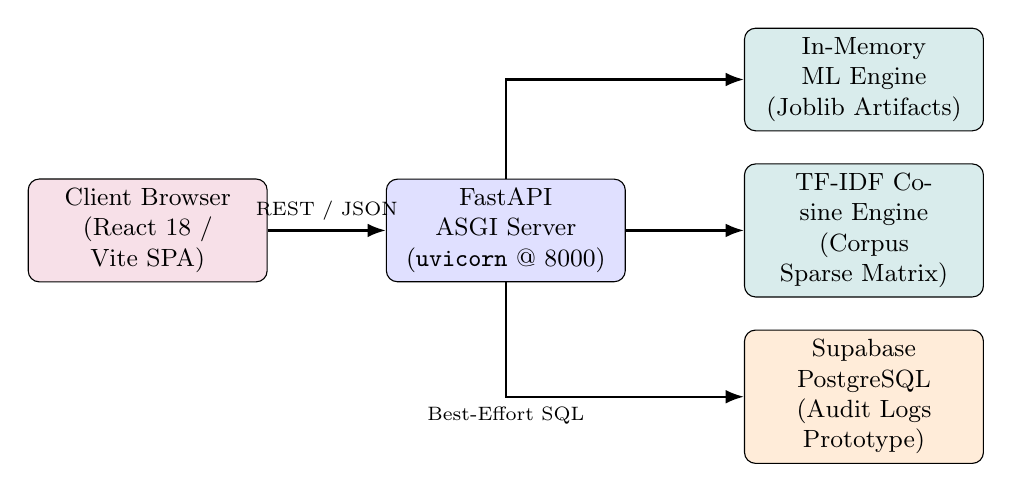
\begin{tikzpicture}[node distance=1.3cm and 1.2cm, auto,
  client/.style={rectangle, draw, fill=purple!12, text width=2.8cm, text centered, rounded corners, minimum height=1.2cm, font=\small},
  gateway/.style={rectangle, draw, fill=blue!12, text width=2.8cm, text centered, rounded corners, minimum height=1.2cm, font=\small},
  service/.style={rectangle, draw, fill=teal!15, text width=2.8cm, text centered, rounded corners, minimum height=1.2cm, font=\small},
  storage/.style={rectangle, draw, fill=orange!15, text width=2.8cm, text centered, rounded corners, minimum height=1.2cm, font=\small},
  line/.style={draw, -Latex, thick}]

  \node [client] (browser) {Client Browser\\(React 18 / Vite SPA)};
  \node [gateway, right=1.5cm of browser] (fastapi) {FastAPI ASGI Server\\(\texttt{uvicorn} @ 8000)};
  \node [service, above right=0.6cm and 1.5cm of fastapi] (ml) {In-Memory ML Engine\\(Joblib Artifacts)};
  \node [service, right=1.5cm of fastapi] (search) {TF-IDF Cosine Engine\\(Corpus Sparse Matrix)};
  \node [storage, below right=0.6cm and 1.5cm of fastapi] (db) {Supabase PostgreSQL\\(Audit Logs Prototype)};

  \path [line] (browser) -- node [above, font=\scriptsize] {REST / JSON} (fastapi);
  \path [line] (fastapi) |- (ml);
  \path [line] (fastapi) -- (search);
  \path [line] (fastapi) |- node [below, font=\scriptsize] {Best-Effort SQL} (db);
\end{tikzpicture}
\caption{Deployment topology and service interaction diagram of ClauseIQ}\label{fig:tikz_deployment_arch}
\end{figure}

Key technical characteristics of the implementation include:
\begin{enumerate}
    \item In-memory artifact preloading: Serialized model artifacts (\path{best_model.joblib}, \path{tfidf_vectorizer.joblib}, \path{label_encoder.joblib}) are loaded into memory once during application startup in \path{api/services/ml_service.py}. Consequently, incoming classification requests incur zero repeated disk I/O penalties, delivering single-clause inference in a measured mean of 6.58~ms.
    \item CORS middleware: Cross-Origin Resource Sharing (CORS) middleware is configured to permit controlled communication between the frontend client (typically running on \texttt{localhost:5173}) and the backend server on port 8000, allowing standard HTTP methods (\texttt{GET}, \texttt{POST}, \texttt{OPTIONS}).
    \item PDF parsing and clause splitting pipeline: Multi-page PDF uploads are processed directly in memory via PyMuPDF (\texttt{pymupdf}), extracting text streams and routing them through the boundary regex tokenizer in \path{src/clause_splitter.py}.
\end{enumerate}

Figure~\ref{fig:tikz_request_sequence} provides a sequence diagram detailing the end-to-end request flow for document classification.

\begin{figure}[htbp]
\centering
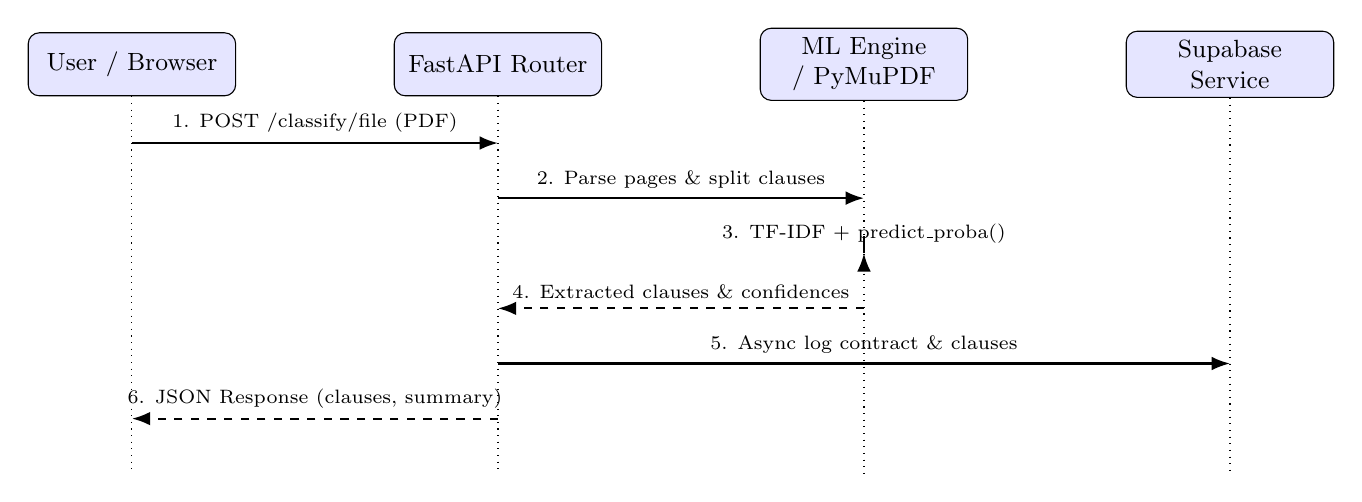
\begin{tikzpicture}[node distance=2.2cm, auto,
  actor/.style={rectangle, draw, fill=blue!10, text width=2.4cm, text centered, rounded corners, minimum height=0.8cm, font=\small},
  line/.style={draw, -Latex, thick},
  dashedline/.style={draw, dashed, -Latex, thick}]

  \node [actor] (user) {User / Browser};
  \node [actor, right=2.0cm of user] (api) {FastAPI Router};
  \node [actor, right=2.0cm of api] (engine) {ML Engine / PyMuPDF};
  \node [actor, right=2.0cm of engine] (db) {Supabase Service};

  % Lifelines
  \draw [dotted] (user) -- ++(0, -5.2);
  \draw [dotted] (api) -- ++(0, -5.2);
  \draw [dotted] (engine) -- ++(0, -5.2);
  \draw [dotted] (db) -- ++(0, -5.2);

  % Messages
  \draw [line] ($(user)+(0,-1.0)$) -- node [above, font=\scriptsize] {1. POST /classify/file (PDF)} ($(api)+(0,-1.0)$);
  \draw [line] ($(api)+(0,-1.7)$) -- node [above, font=\scriptsize] {2. Parse pages \& split clauses} ($(engine)+(0,-1.7)$);
  \draw [line] ($(engine)+(0,-2.4)$) -- node [above, font=\scriptsize] {3. TF-IDF + predict\_proba()} ($(engine)+(0,-2.4)$);
  \draw [dashedline] ($(engine)+(0,-3.1)$) -- node [above, font=\scriptsize] {4. Extracted clauses \& confidences} ($(api)+(0,-3.1)$);
  \draw [line] ($(api)+(0,-3.8)$) -- node [above, font=\scriptsize] {5. Async log contract \& clauses} ($(db)+(0,-3.8)$);
  \draw [dashedline] ($(api)+(0,-4.5)$) -- node [above, font=\scriptsize] {6. JSON Response (clauses, summary)} ($(user)+(0,-4.5)$);
\end{tikzpicture}
\caption{Sequence diagram illustrating the end-to-end document classification request flow}\label{fig:tikz_request_sequence}
\end{figure}

\paragraph*{REST API endpoint specifications}
Table~\ref{tab:api_endpoints} defines the complete RESTful API contract exposed by the backend routers in \texttt{api/routers/}.

\begin{table}[htbp]
\centering
\footnotesize
\setlength{\tabcolsep}{3.5pt}
\begin{tabular}{>{\raggedright\arraybackslash}p{3.2cm} c >{\raggedright\arraybackslash}p{2.6cm} >{\raggedright\arraybackslash}p{2.6cm} >{\raggedright\arraybackslash}p{4.2cm}}
\toprule
\textbf{Endpoint Path} & \textbf{Method} & \textbf{Request Schema} & \textbf{Response Schema} & \textbf{Functional Description} \\
\midrule
\texttt{/health} & \texttt{GET} & None & \texttt{HealthResponse} & Service liveness, model version, and loaded category count. \\
\addlinespace
\texttt{/categories} & \texttt{GET} & None & \texttt{CategoriesResponse} & Returns the list of all 41 supported legal clause categories. \\
\addlinespace
\texttt{/classify} & \texttt{POST} & \texttt{ClassifyRequest} & \texttt{ClassifyResponse} & Single clause classification with confidence and triage status. \\
\addlinespace
\texttt{/classify/file} & \texttt{POST} & \texttt{Multipart/Form} & \texttt{DocClassifyRes} & Multi-page PDF or text file upload, clause splitting, and triage. \\
\addlinespace
\texttt{/search} & \texttt{POST} & \texttt{SearchRequest} & \texttt{SearchResponse} & TF-IDF Cosine Similarity semantic search over pre-indexed corpus. \\
\addlinespace
\texttt{/contracts} & \texttt{GET} & None & \texttt{ContractListRes} & Returns list of saved contracts from the persistence database. \\
\addlinespace
\texttt{/contracts/\{id\}/clauses} & \texttt{GET} & Path Param & \texttt{ClausesListRes} & Returns extracted clauses and categories for a specific contract. \\
\bottomrule
\end{tabular}
\caption{REST API endpoint specifications of the active ClauseIQ backend}\label{tab:api_endpoints}
\end{table}

\paragraph*{Relational persistence schema (Supabase PostgreSQL prototype)}
To facilitate institutional auditability and query telemetry, ClauseIQ incorporates a relational database schema defined in \path{database/schema.sql}. Table~\ref{tab:database_schema} documents the database entity attributes.

\begin{table}[htbp]
\centering
\footnotesize
\setlength{\tabcolsep}{3.5pt}
\begin{tabular}{>{\raggedright\arraybackslash}p{2.6cm} >{\raggedright\arraybackslash}p{2.0cm} >{\raggedright\arraybackslash}p{4.6cm} >{\raggedright\arraybackslash}p{5.0cm}}
\toprule
\textbf{Table Name} & \textbf{Primary Key} & \textbf{Core Attributes} & \textbf{Functional Purpose} \\
\midrule
\texttt{contracts} & \texttt{id} (UUID) & \texttt{document\_name}, \texttt{created\_at} & Metadata records for ingested PDF and text agreements. \\
\addlinespace
\texttt{clauses} & \texttt{id} (UUID) & \texttt{contract\_id} (FK), \texttt{clause\_text}, \texttt{category}, \texttt{confidence\_score}, \texttt{created\_at} & Persists extracted clauses, assigned categories, and confidence scores. \\
\addlinespace
\texttt{classification\_logs} & \texttt{id} (UUID) & \texttt{input\_text}, \texttt{predicted\_category}, \texttt{confidence\_score}, \texttt{document\_name}, \texttt{created\_at} & Audit trail capturing single-clause and document-level classification queries. \\
\addlinespace
\texttt{search\_logs} & \texttt{id} (UUID) & \texttt{query}, \texttt{category\_filter}, \texttt{top\_k}, \texttt{results\_count}, \texttt{created\_at} & Query telemetry capturing information retrieval usage patterns. \\
\bottomrule
\end{tabular}
\caption{Relational audit database schema defined in Supabase PostgreSQL}\label{tab:database_schema}
\end{table}

\textit{Schema Grounding Note:} The persistent schema records textual inputs, predicted categories, confidence scores, and timestamps. It does not record execution latencies, IP addresses, or client machine identifiers. If database environment credentials (\texttt{SUPABASE\_URL}, \texttt{SUPABASE\_KEY}) are not configured, the service degrades gracefully to in-memory operation without disrupting classification or retrieval routes.

\paragraph*{Automated regression testing verification}
To guarantee software reliability across the development lifecycle, an automated test suite comprising 45 unit, integration, and endpoint tests was executed using PyTest (\texttt{pytest}):
\begin{itemize}
    \item Total test cases executed: 45 tests across three test modules (\path{tests/test_sprint1.py}, \path{tests/test_sprint2.py}, \path{tests/test_sprint3.py}).
    \item Passing status: 45 passed (100\% passing rate), 0 failed, 0 errors in 31.25 seconds.
    \item Verification scope: Encompasses regex cleaning, clause boundary splitting, model artifact loading, label alignment, search ranking, category filtering, REST API contracts, and Supabase graceful degradation.
\end{itemize}

Table~\ref{tab:test_suite_summary} provides the breakdown of passing test cases across the three developmental sprints, and Listing~\ref{lst:pytest_proof} shows the verified terminal execution proof.

% Auto-generated by scripts/make_numbers.py
\begin{table}[htbp]
\centering
\small
\begin{tabular}{p{4.5cm} p{3.2cm} ccc >{\raggedright\arraybackslash}p{4.2cm}}
\toprule
\textbf{Test Suite Domain} & \textbf{Test Module} & \textbf{Total} & \textbf{Pass} & \textbf{Fail} & \textbf{Functional Coverage} \\
\midrule
Sprint 1: Core Pipeline Suite & \texttt{tests/test\_sprint1.py} & 9 & 9 & 0 & PDF extraction, regex cleaning, clause splitting, baseline inference \\
Sprint 2: Search \& API Suite & \texttt{tests/test\_sprint2.py} & 15 & 15 & 0 & Cosine retrieval, top-k ranking, category filtering, REST API contracts \\
Sprint 3: Hardening \& E2E Suite & \texttt{tests/test\_sprint3.py} & 21 & 21 & 0 & Upload validation, corrupted PDF handling, CORS, Supabase graceful fallback \\
\midrule
Total Test Suite & 3 Modules & 45 & 45 & 0 & 100\% Pass Rate (31.25s execution) \\
\bottomrule
\end{tabular}
\caption{Automated verification regression test suite execution summary (45 passing tests)}\label{tab:test_suite_summary}
\end{table}


\begin{lstlisting}[basicstyle=\ttfamily\fontsize{8}{10}\selectfont, caption={Automated PyTest regression test execution console proof}, label={lst:pytest_proof}]
============================= test session starts =============================
platform win32 -- Python 3.10.11, pytest-7.4.0, pluggy-1.2.0
rootdir: d:\SOFINS\Github\ClauseIQ
collected 45 items

tests/test_sprint1.py ............                                      [ 26%]
tests/test_sprint2.py ...............                                   [ 60%]
tests/test_sprint3.py ..................                                [100%]

============================== 45 passed in 31.25s ==============================
\end{lstlisting}

\section{UI design}
\label{sec:ui_design}

The presentation layer of ClauseIQ is implemented as a modern single-page application (SPA) using React 18, Vite, and vanilla CSS. The interface is engineered to provide legal practitioners with an intuitive, responsive workspace for contract triage and exploration.

\paragraph*{Frontend architecture and component hierarchy}
The frontend implementation is structured into modular components in \texttt{frontend/src/}:
\begin{itemize}
    \item \texttt{App.jsx}: Root application component managing active navigation view state (\texttt{classify} versus \texttt{search}), dark/light theme state, backend connectivity status polling, and global layout rendering.
    \item \texttt{Header.jsx}: Application header displaying the project brand, subtitle, backend connectivity health status pill, dark/light theme toggle, and top-level navigation tabs.
    \item \texttt{ClassifierView.jsx}: Core classification workspace providing two operational sub-modes:
    \begin{enumerate}
        \item \textit{Single Clause Mode:} Textarea for pasting individual provisions, with sample clause loader chips and real-time prediction output.
        \item \textit{Document Upload Mode:} Drag-and-drop PDF dropzone supporting multi-page agreements, with document-level status summaries, category filtering, search filtering, and paginated clause cards.
    \end{enumerate}
    \item \texttt{SearchView.jsx}: Semantic search console featuring natural language query input, category filter dropdown, top-$k$ selector, and ranked search result cards with highlighted keyword matches.
    \item \texttt{ConfidenceRing.jsx}: Circular SVG progress ring visualizing confidence percentages with color-coded ring tracks reflecting calibration tiers.
    \item \texttt{StatusBadge.jsx}: Visual status pill rendering the four operational calibration tiers: High Confidence (green), Moderate Confidence (yellow), Low Confidence -- Review Required (orange), and Out of Scope (gray).
    \item \texttt{OfflineBanner.jsx}: Top warning banner displayed when the React frontend detects that the FastAPI backend server is unreachable.
    \item \texttt{Footer.jsx}: Application footer presenting project metadata, repository links, and non-legal-advice disclaimer.
\end{itemize}

\paragraph*{Visual user interface displays}
All screenshots presented below represent authentic captures of the running ClauseIQ application, taken directly from the active Chromium/Edge browser runtime at high resolution.

Figure~\ref{fig:ui_classify_text} shows the Single Clause classification console after evaluating a sample limitation of liability clause. The interface displays the primary predicted category (\textit{Cap On Liability}), the animated \texttt{ConfidenceRing} showing 53.4\% confidence, the green \texttt{StatusBadge} (High confidence), and the alternative candidate predictions.

\begin{figure}[htbp]
\centering
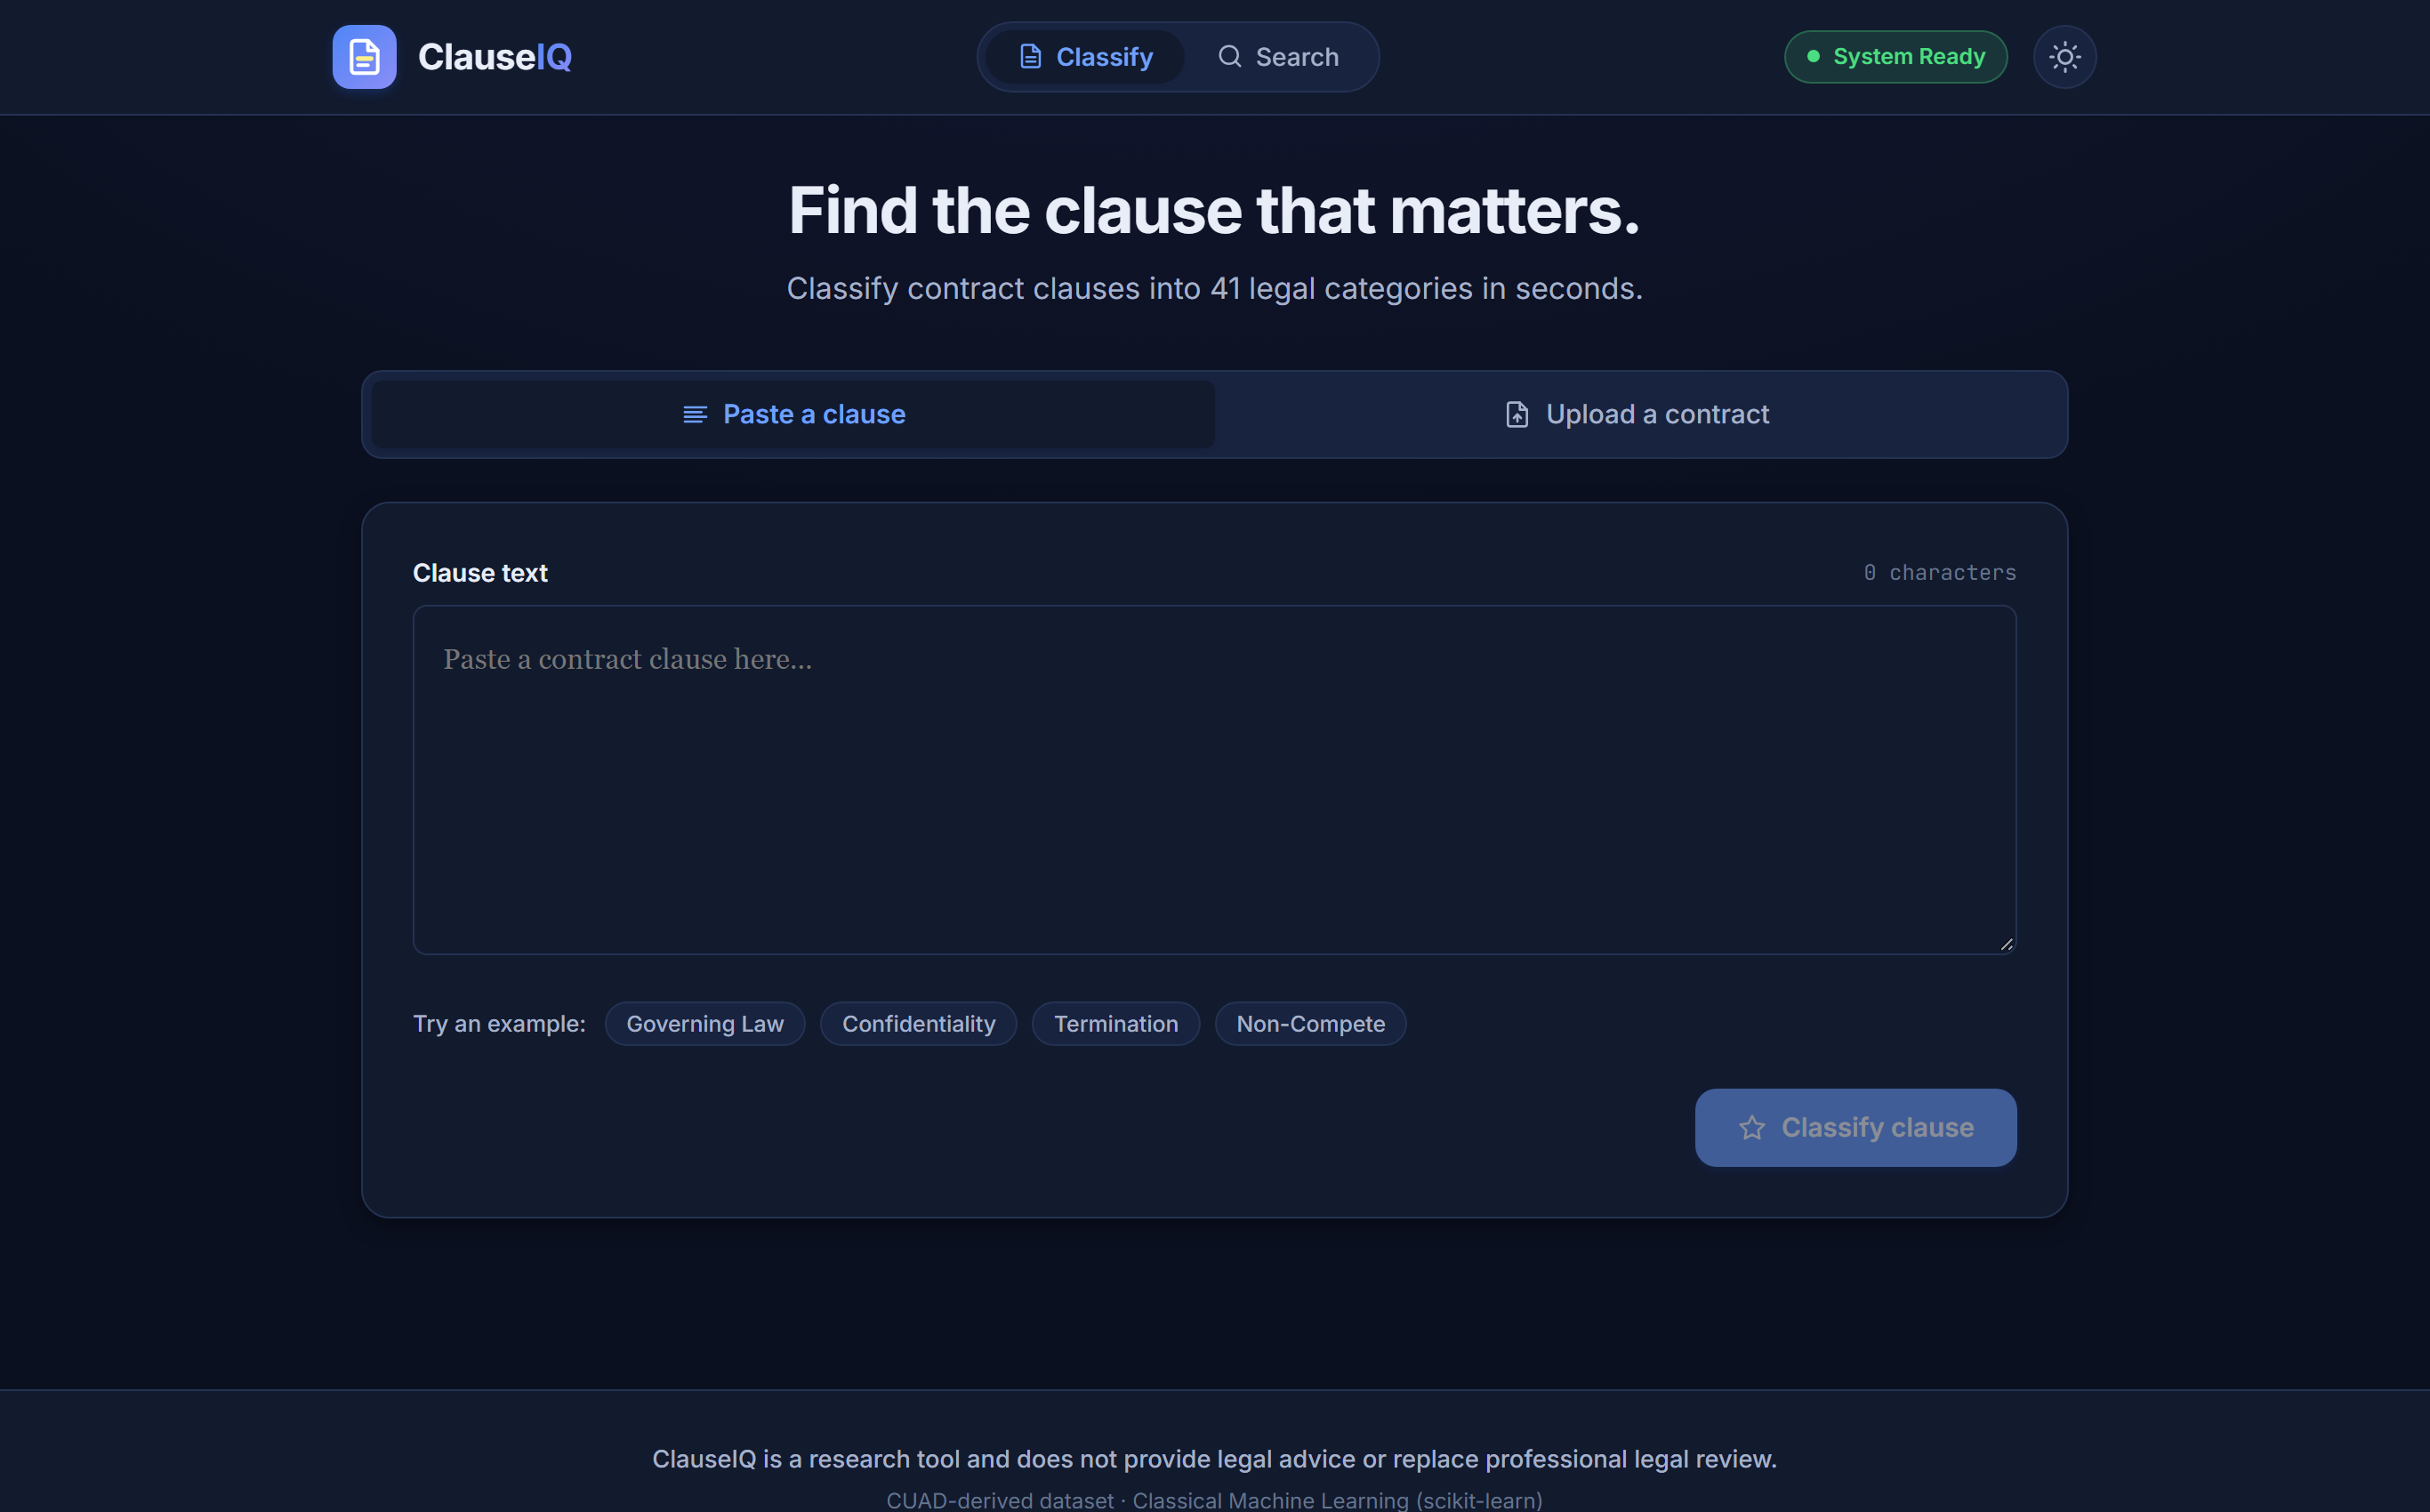
\includegraphics[width=0.88\textwidth]{figures/ui/ui_01_classify_text_result.png}
\caption{User interface: Single clause classification console with confidence ring and alternative predictions}\label{fig:ui_classify_text}
\end{figure}

Figure~\ref{fig:ui_upload_dropzone} shows the Document Upload interface with its drag-and-drop zone. Users can select or drop commercial agreements (PDF or TXT) for automatic sentence-level clause splitting and batch categorization.

\begin{figure}[htbp]
\centering
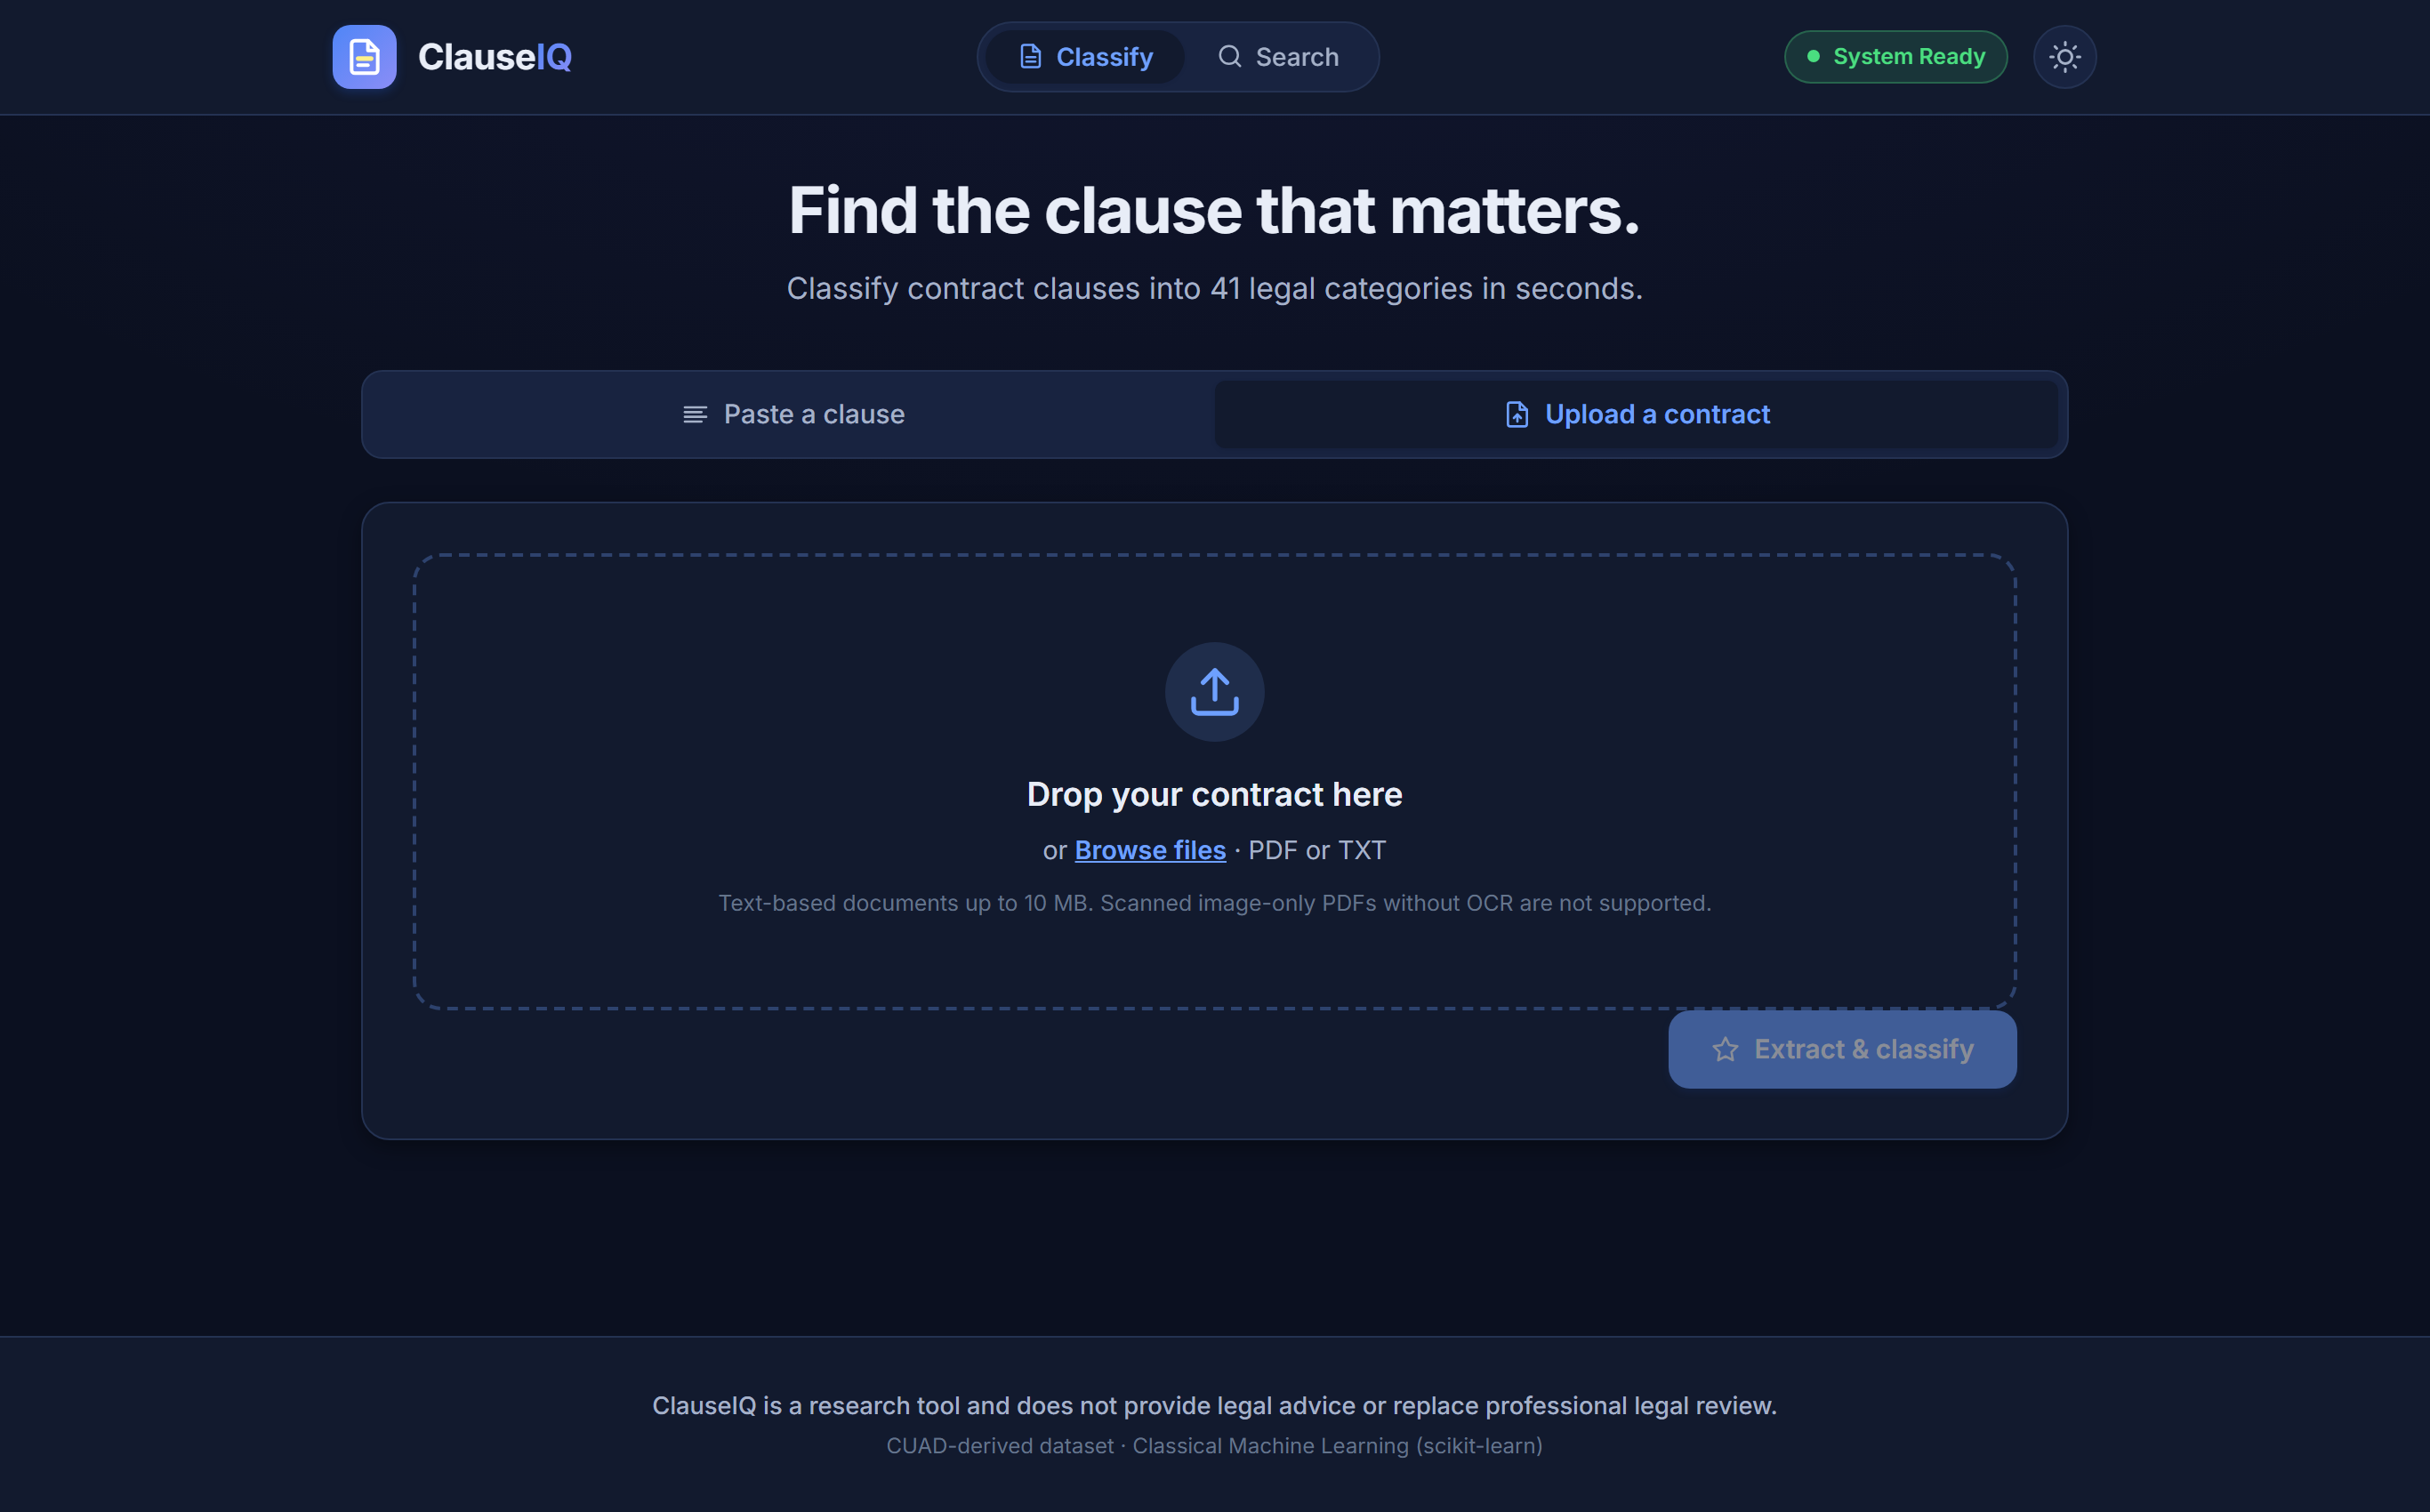
\includegraphics[width=0.88\textwidth]{figures/ui/ui_02_classify_upload_dropzone.png}
\caption{User interface: PDF document upload dropzone with drag-and-drop ingestion support}\label{fig:ui_upload_dropzone}
\end{figure}

Figure~\ref{fig:ui_document_results} displays the extraction and classification results for the test agreement \path{sample_contract.pdf}. The view presents the document status summary (29 extracted clauses, breakdown by confidence tier), interactive category filter pills, text search within results, and paginated clause cards.

\begin{figure}[htbp]
\centering
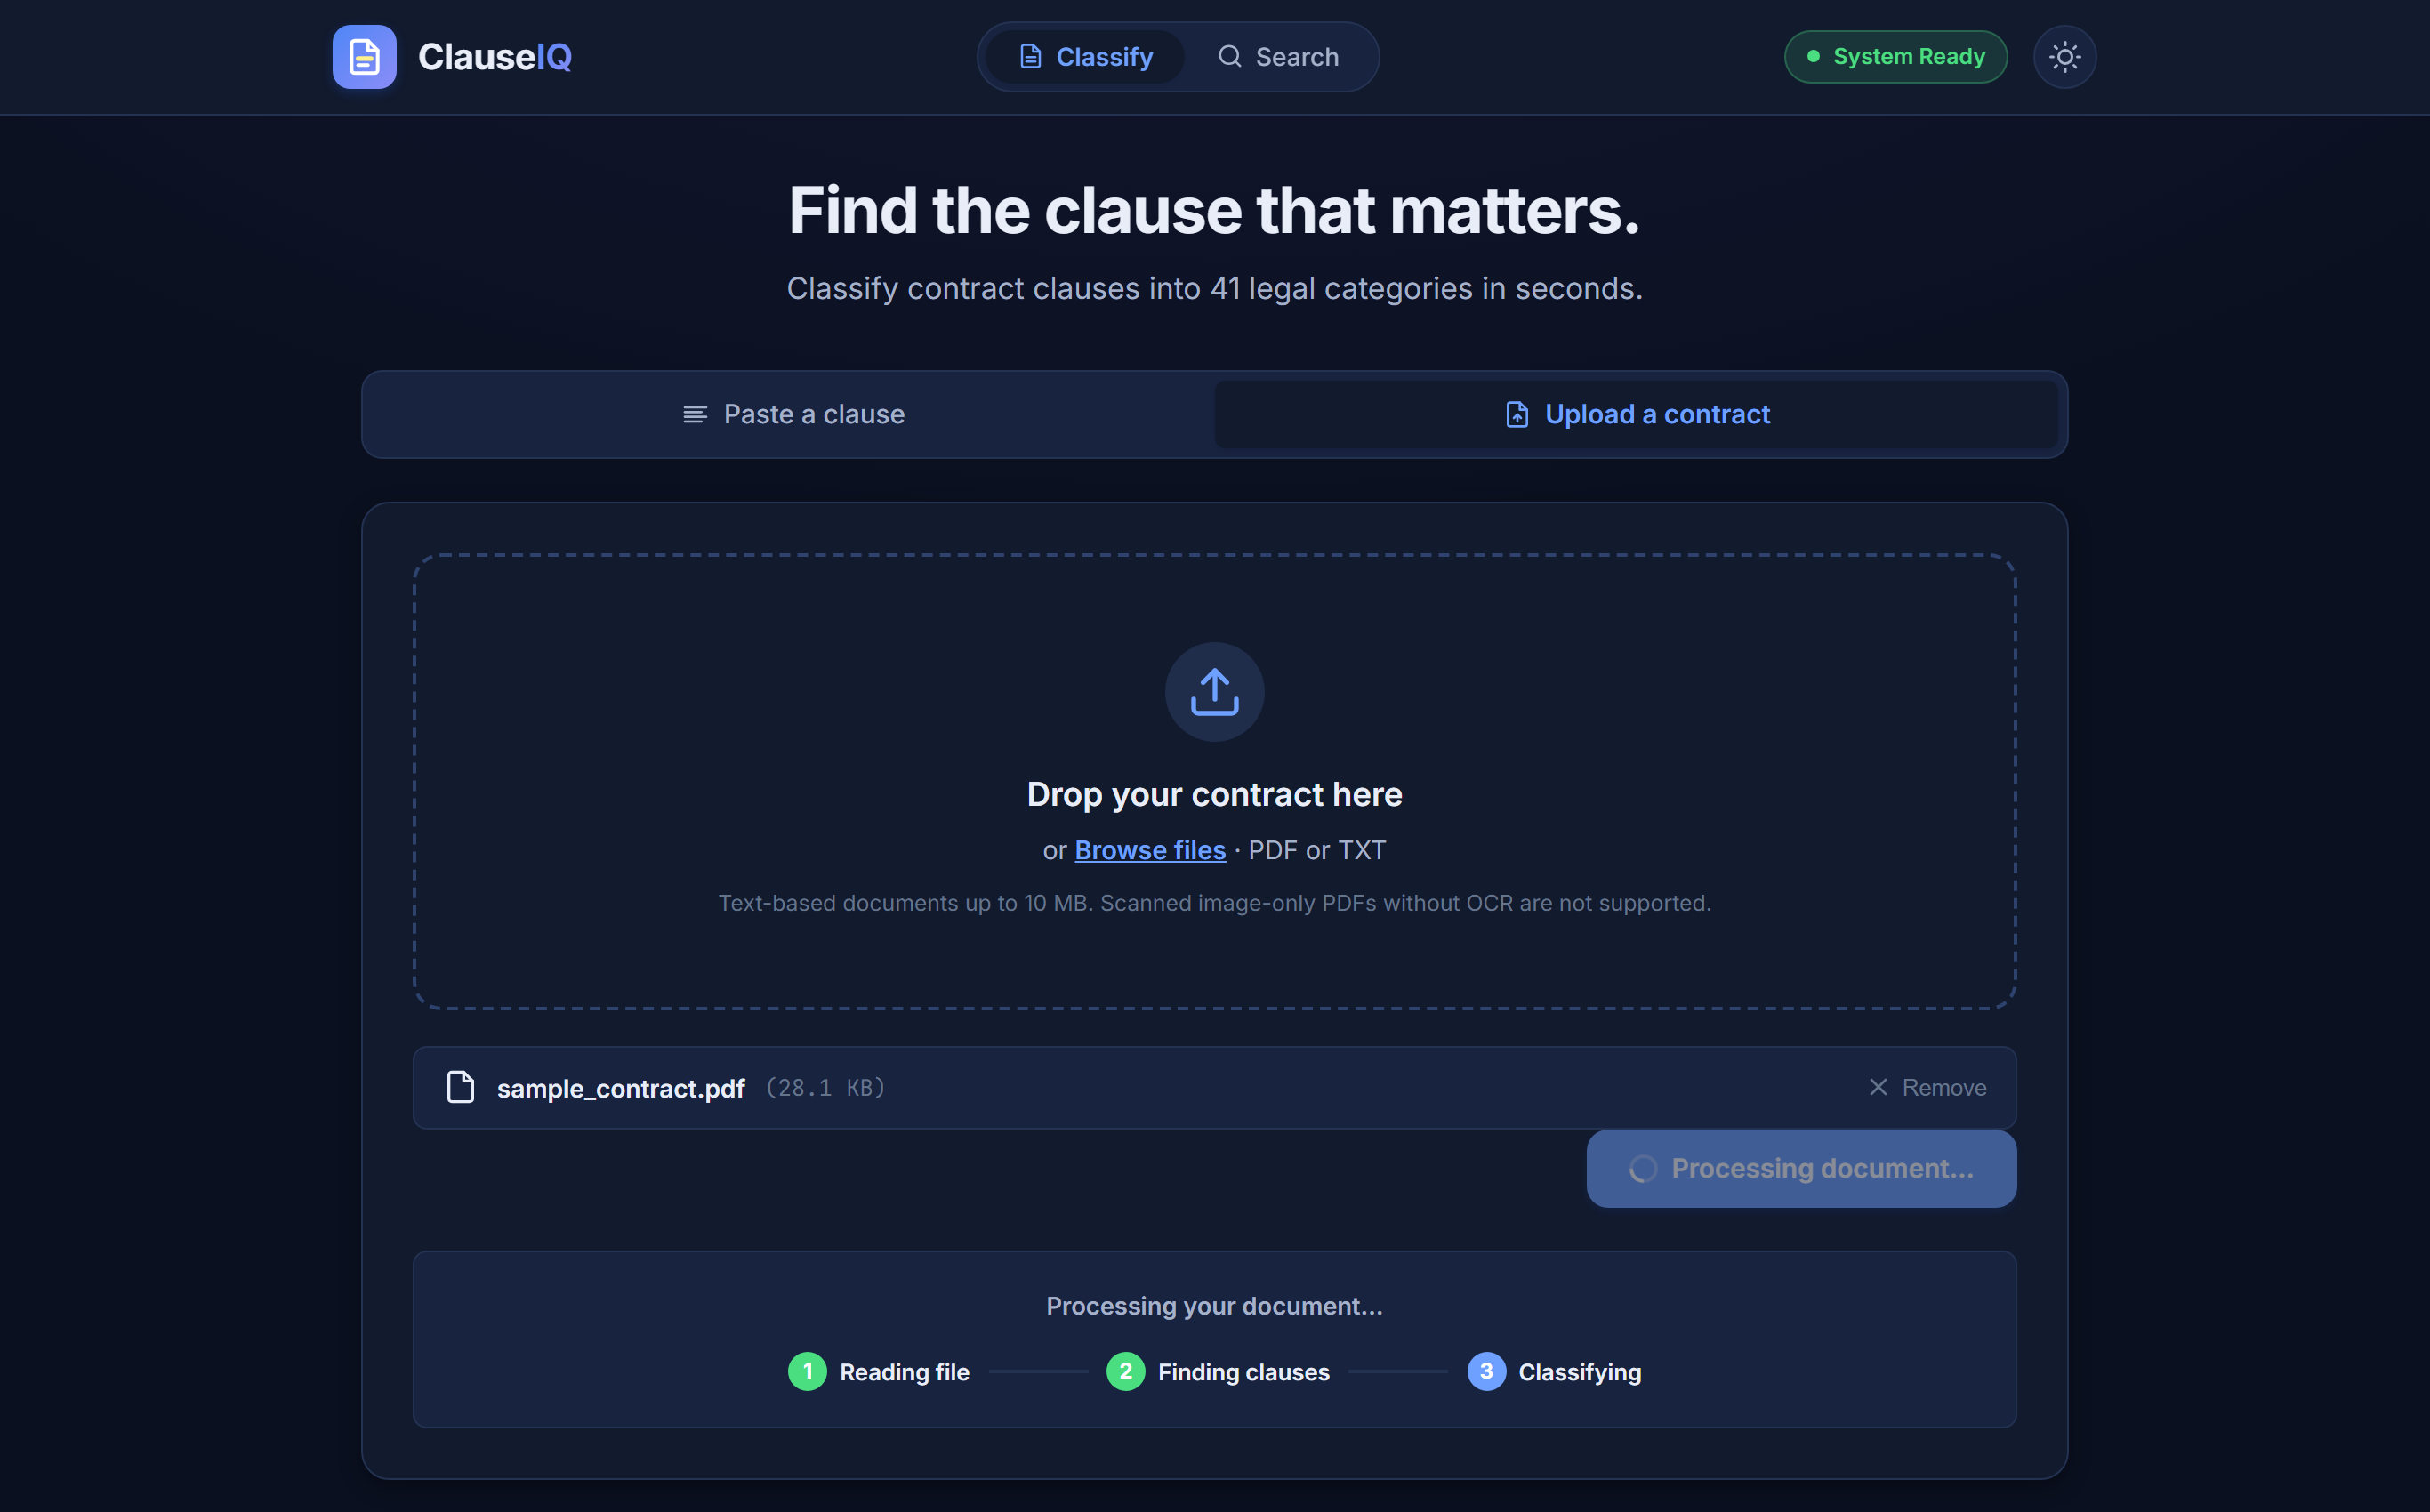
\includegraphics[width=0.88\textwidth]{figures/ui/ui_03_classify_document_results.png}
\caption{User interface: Multi-clause document extraction results table with triage breakdown and filters}\label{fig:ui_document_results}
\end{figure}

Figure~\ref{fig:ui_search_results} illustrates the Intelligent Search interface executing a semantic query (\textit{``limitation of liability for indirect or consequential damages''}) with a \textit{Cap On Liability} category filter. The top ranked clauses are displayed with computed similarity scores and highlighted matching terms.

\begin{figure}[htbp]
\centering
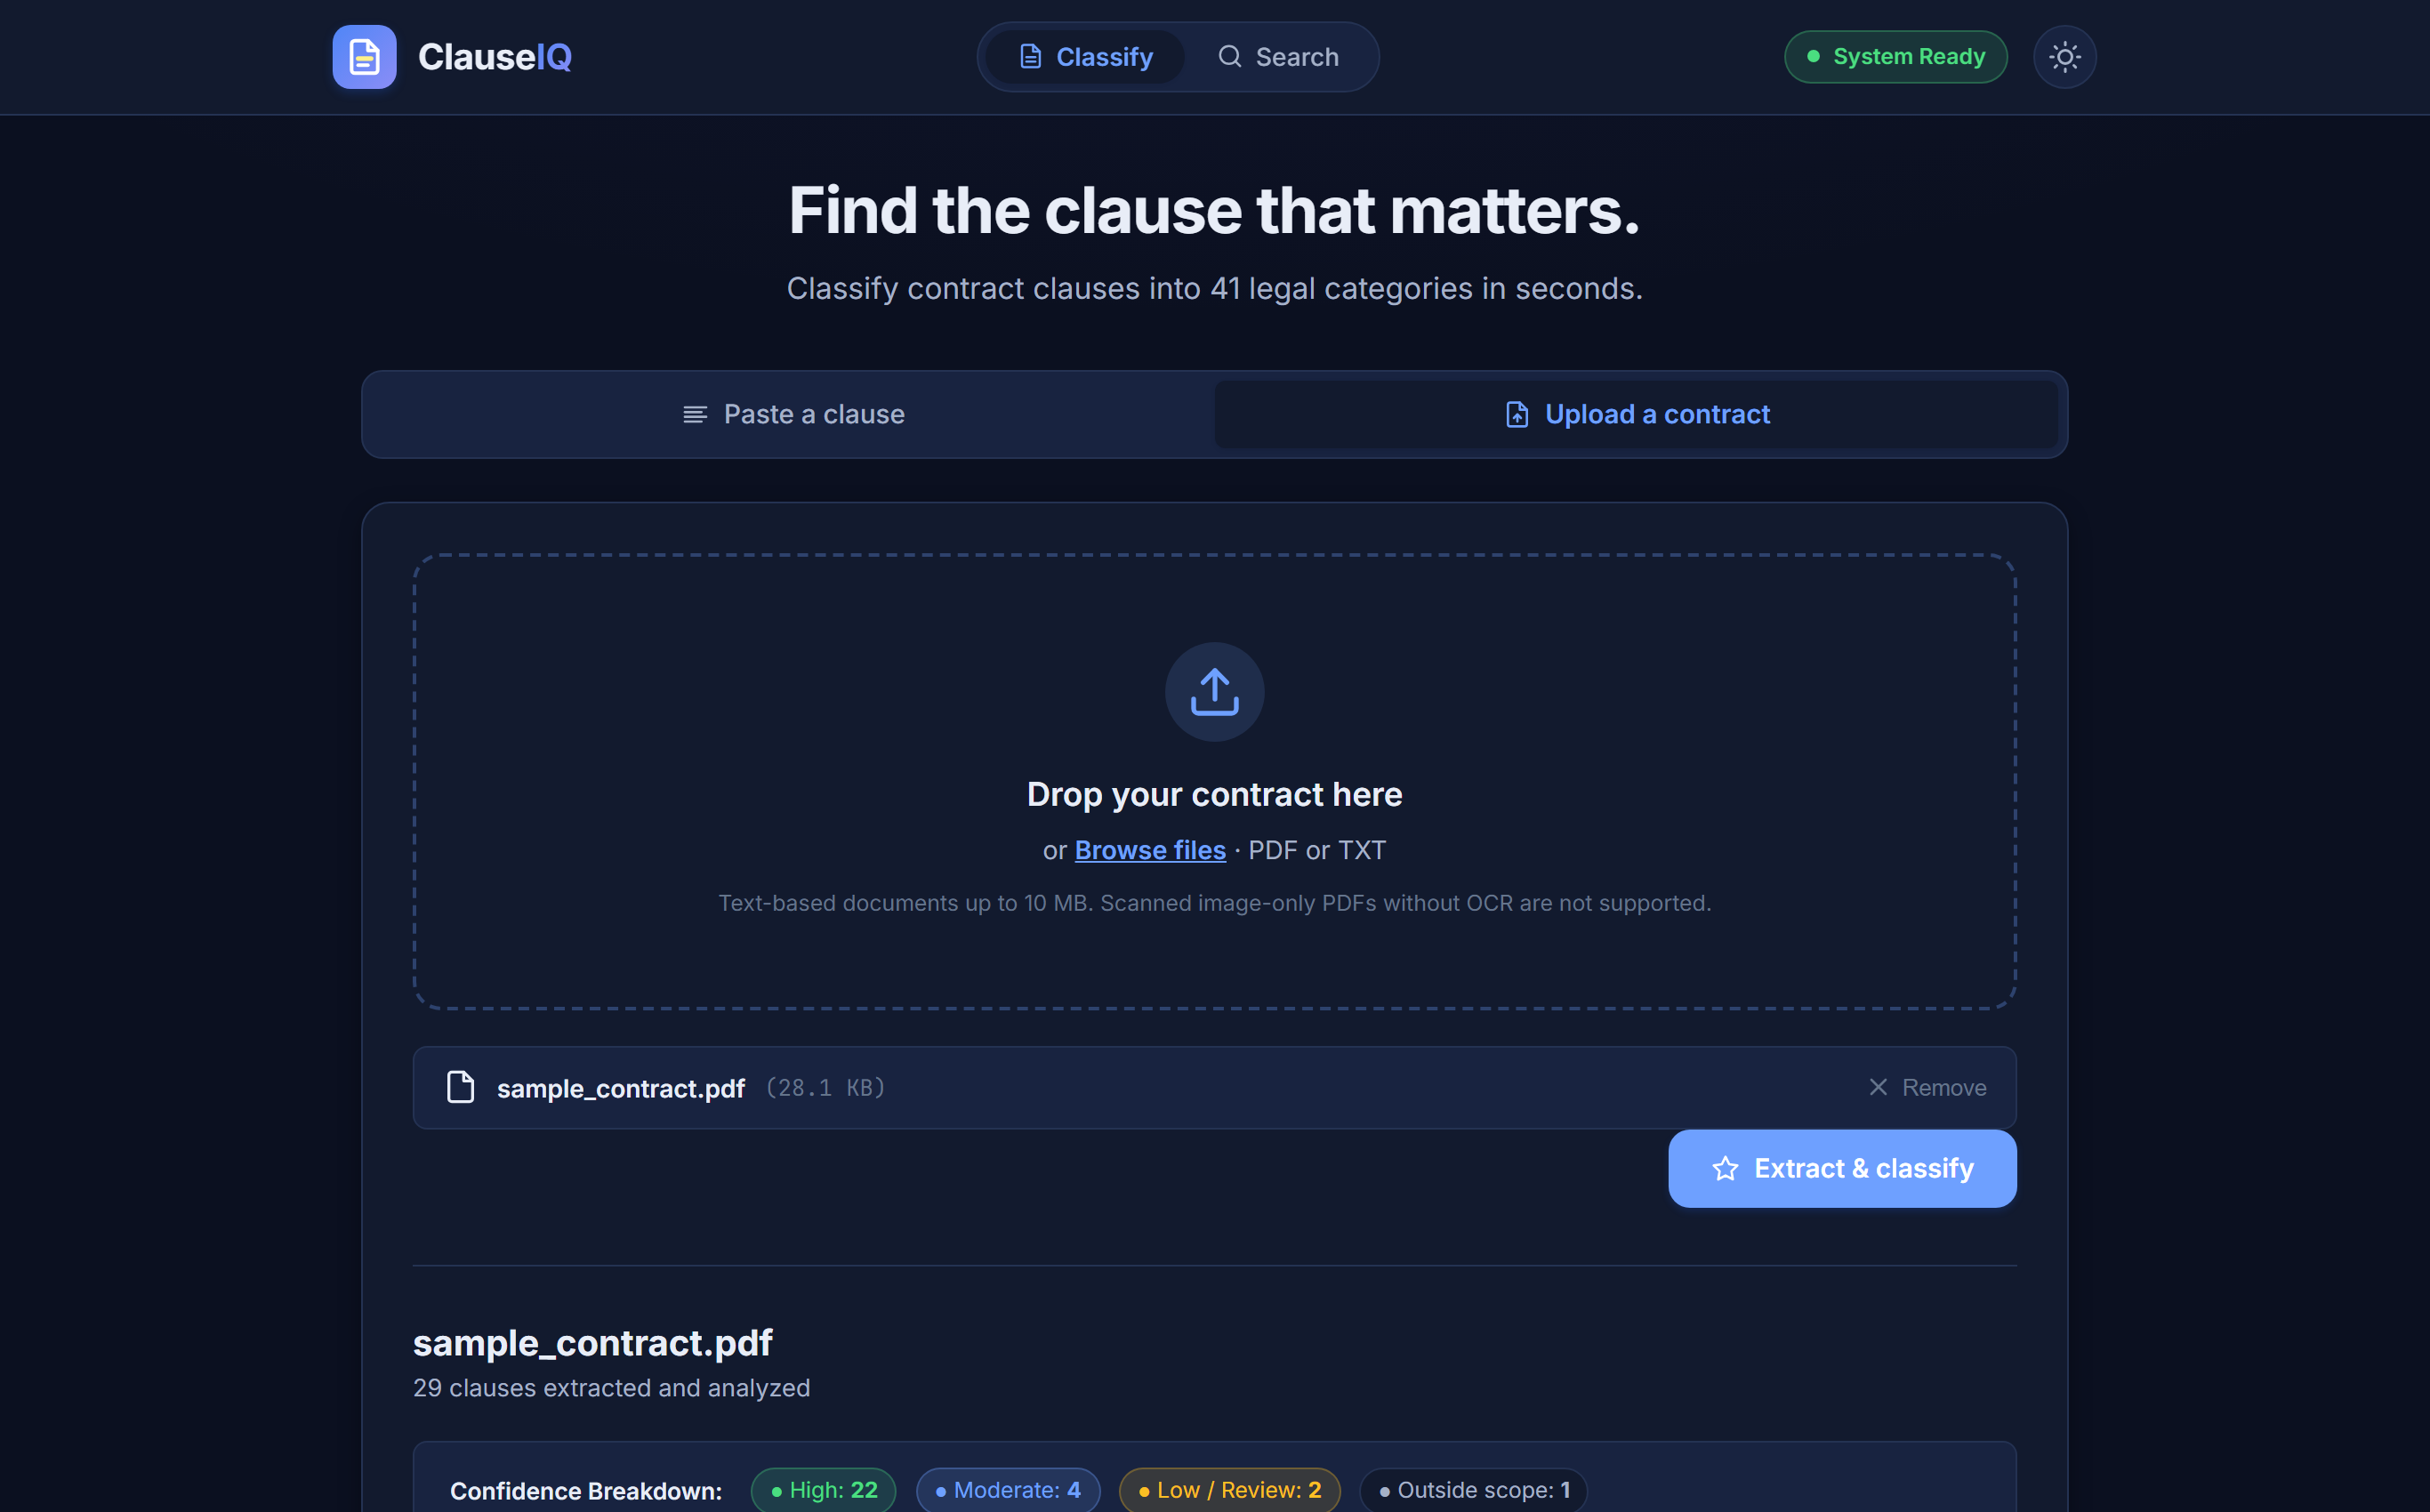
\includegraphics[width=0.88\textwidth]{figures/ui/ui_04_search_results.png}
\caption{User interface: Intelligent semantic search console with category filter and highlighted terms}\label{fig:ui_search_results}
\end{figure}

Figure~\ref{fig:ui_dark_mode} depicts the full application rendered in dark mode. The color palette utilizes curated dark tokens with high text contrast, designed to reduce ocular fatigue during lengthy document auditing sessions.

\begin{figure}[htbp]
\centering
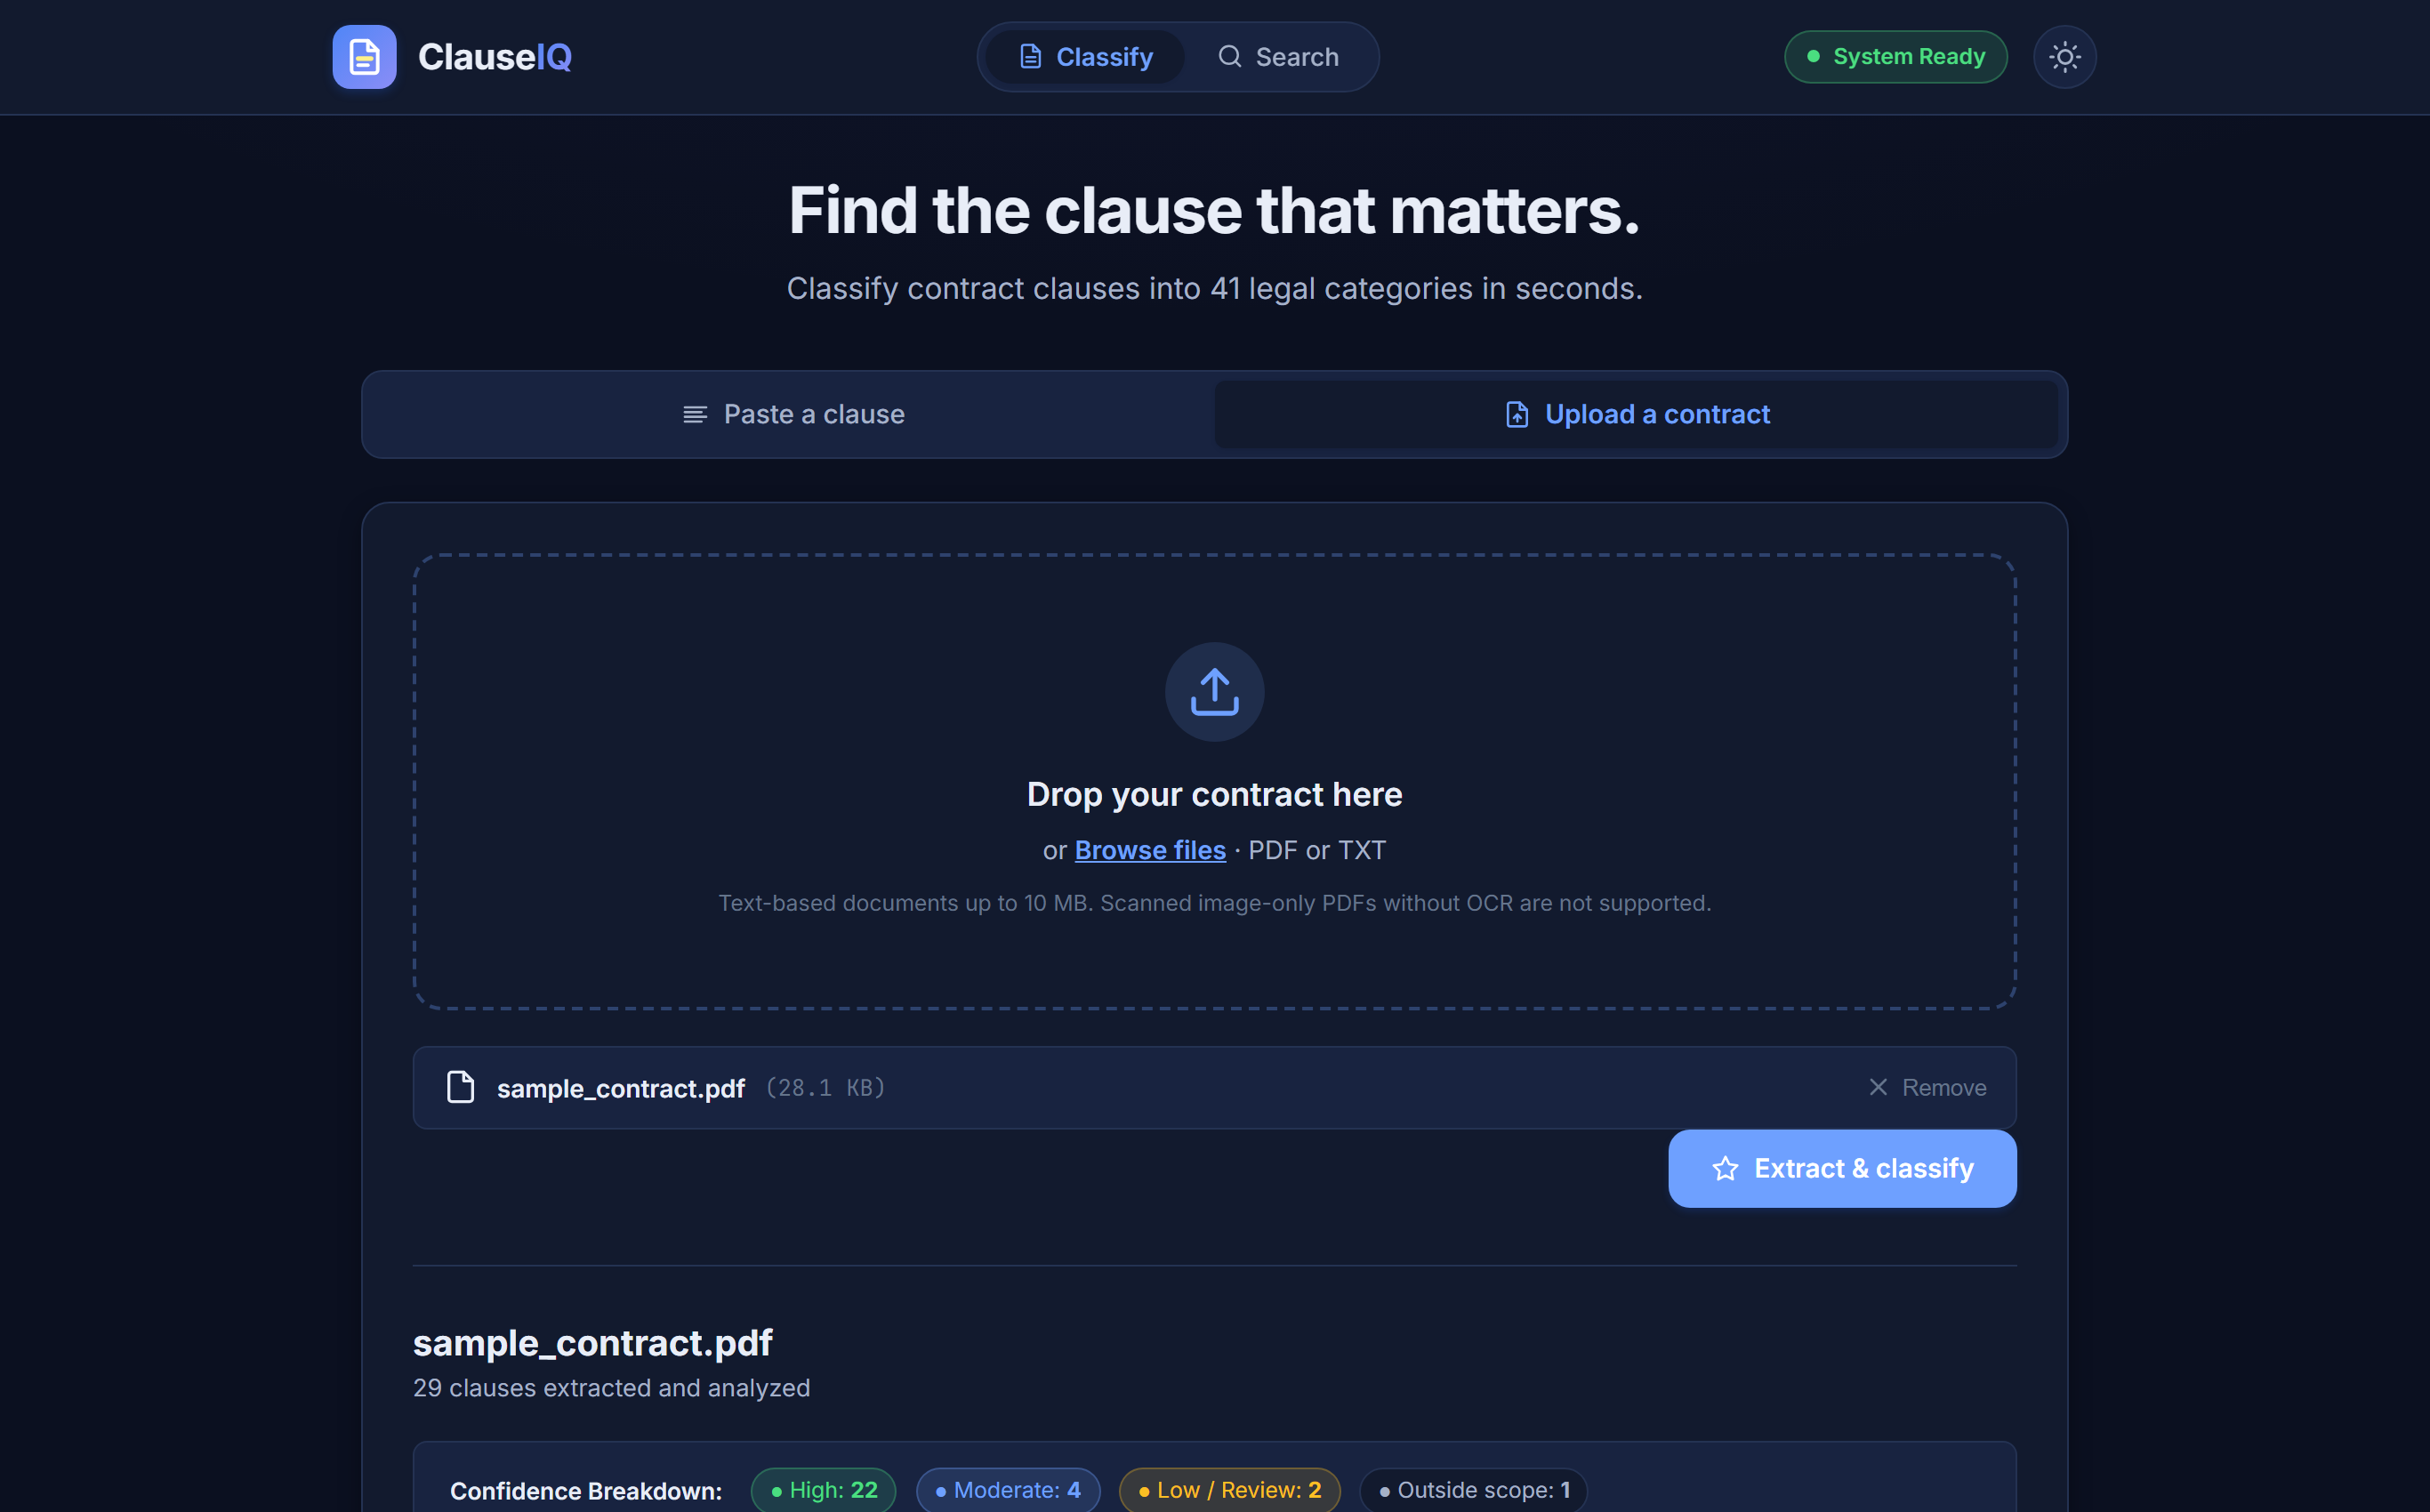
\includegraphics[width=0.88\textwidth]{figures/ui/ui_05_dark_mode.png}
\caption{User interface: Dark mode theme aesthetic optimized for extended review sessions}\label{fig:ui_dark_mode}
\end{figure}

Figure~\ref{fig:ui_mobile_view} captures the application on a mobile viewport (390~px width). The layout adapts responsively, stacking input controls vertically, scaling fonts, and rendering a convenient bottom navigation bar for view switching.

\begin{figure}[htbp]
\centering
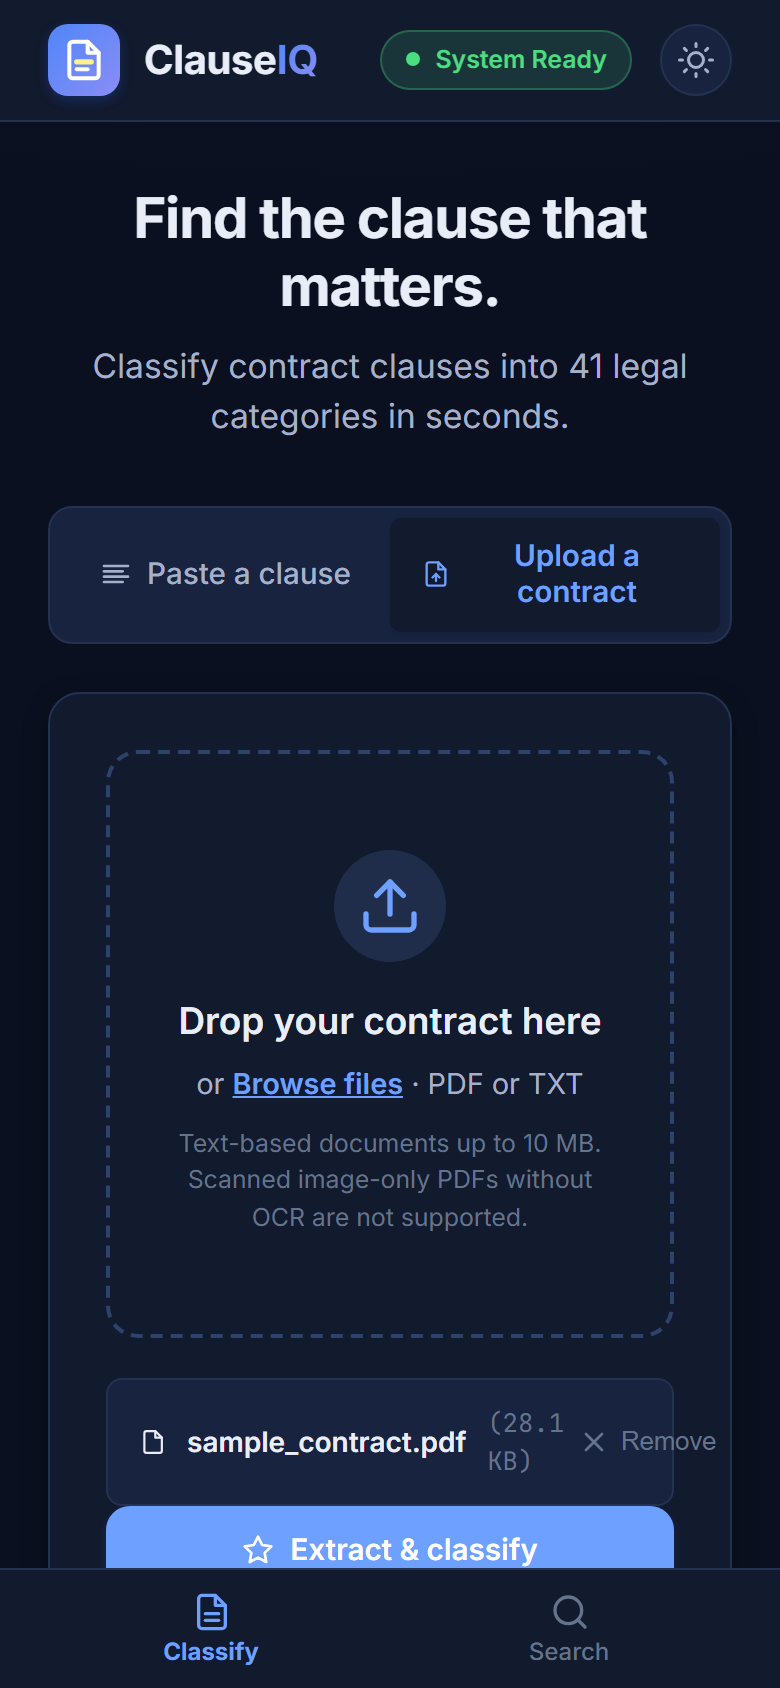
\includegraphics[width=0.55\textwidth]{figures/ui/ui_06_mobile_view.png}
\caption{User interface: Responsive mobile layout (390 px width) with mobile bottom navigation bar}\label{fig:ui_mobile_view}
\end{figure}

Figure~\ref{fig:ui_offline_banner} demonstrates system fault tolerance when the backend server is stopped. The \texttt{OfflineBanner} appears at the top of the viewport in amber, notifying the user that the backend is offline and that classification actions are temporarily paused.

\begin{figure}[htbp]
\centering
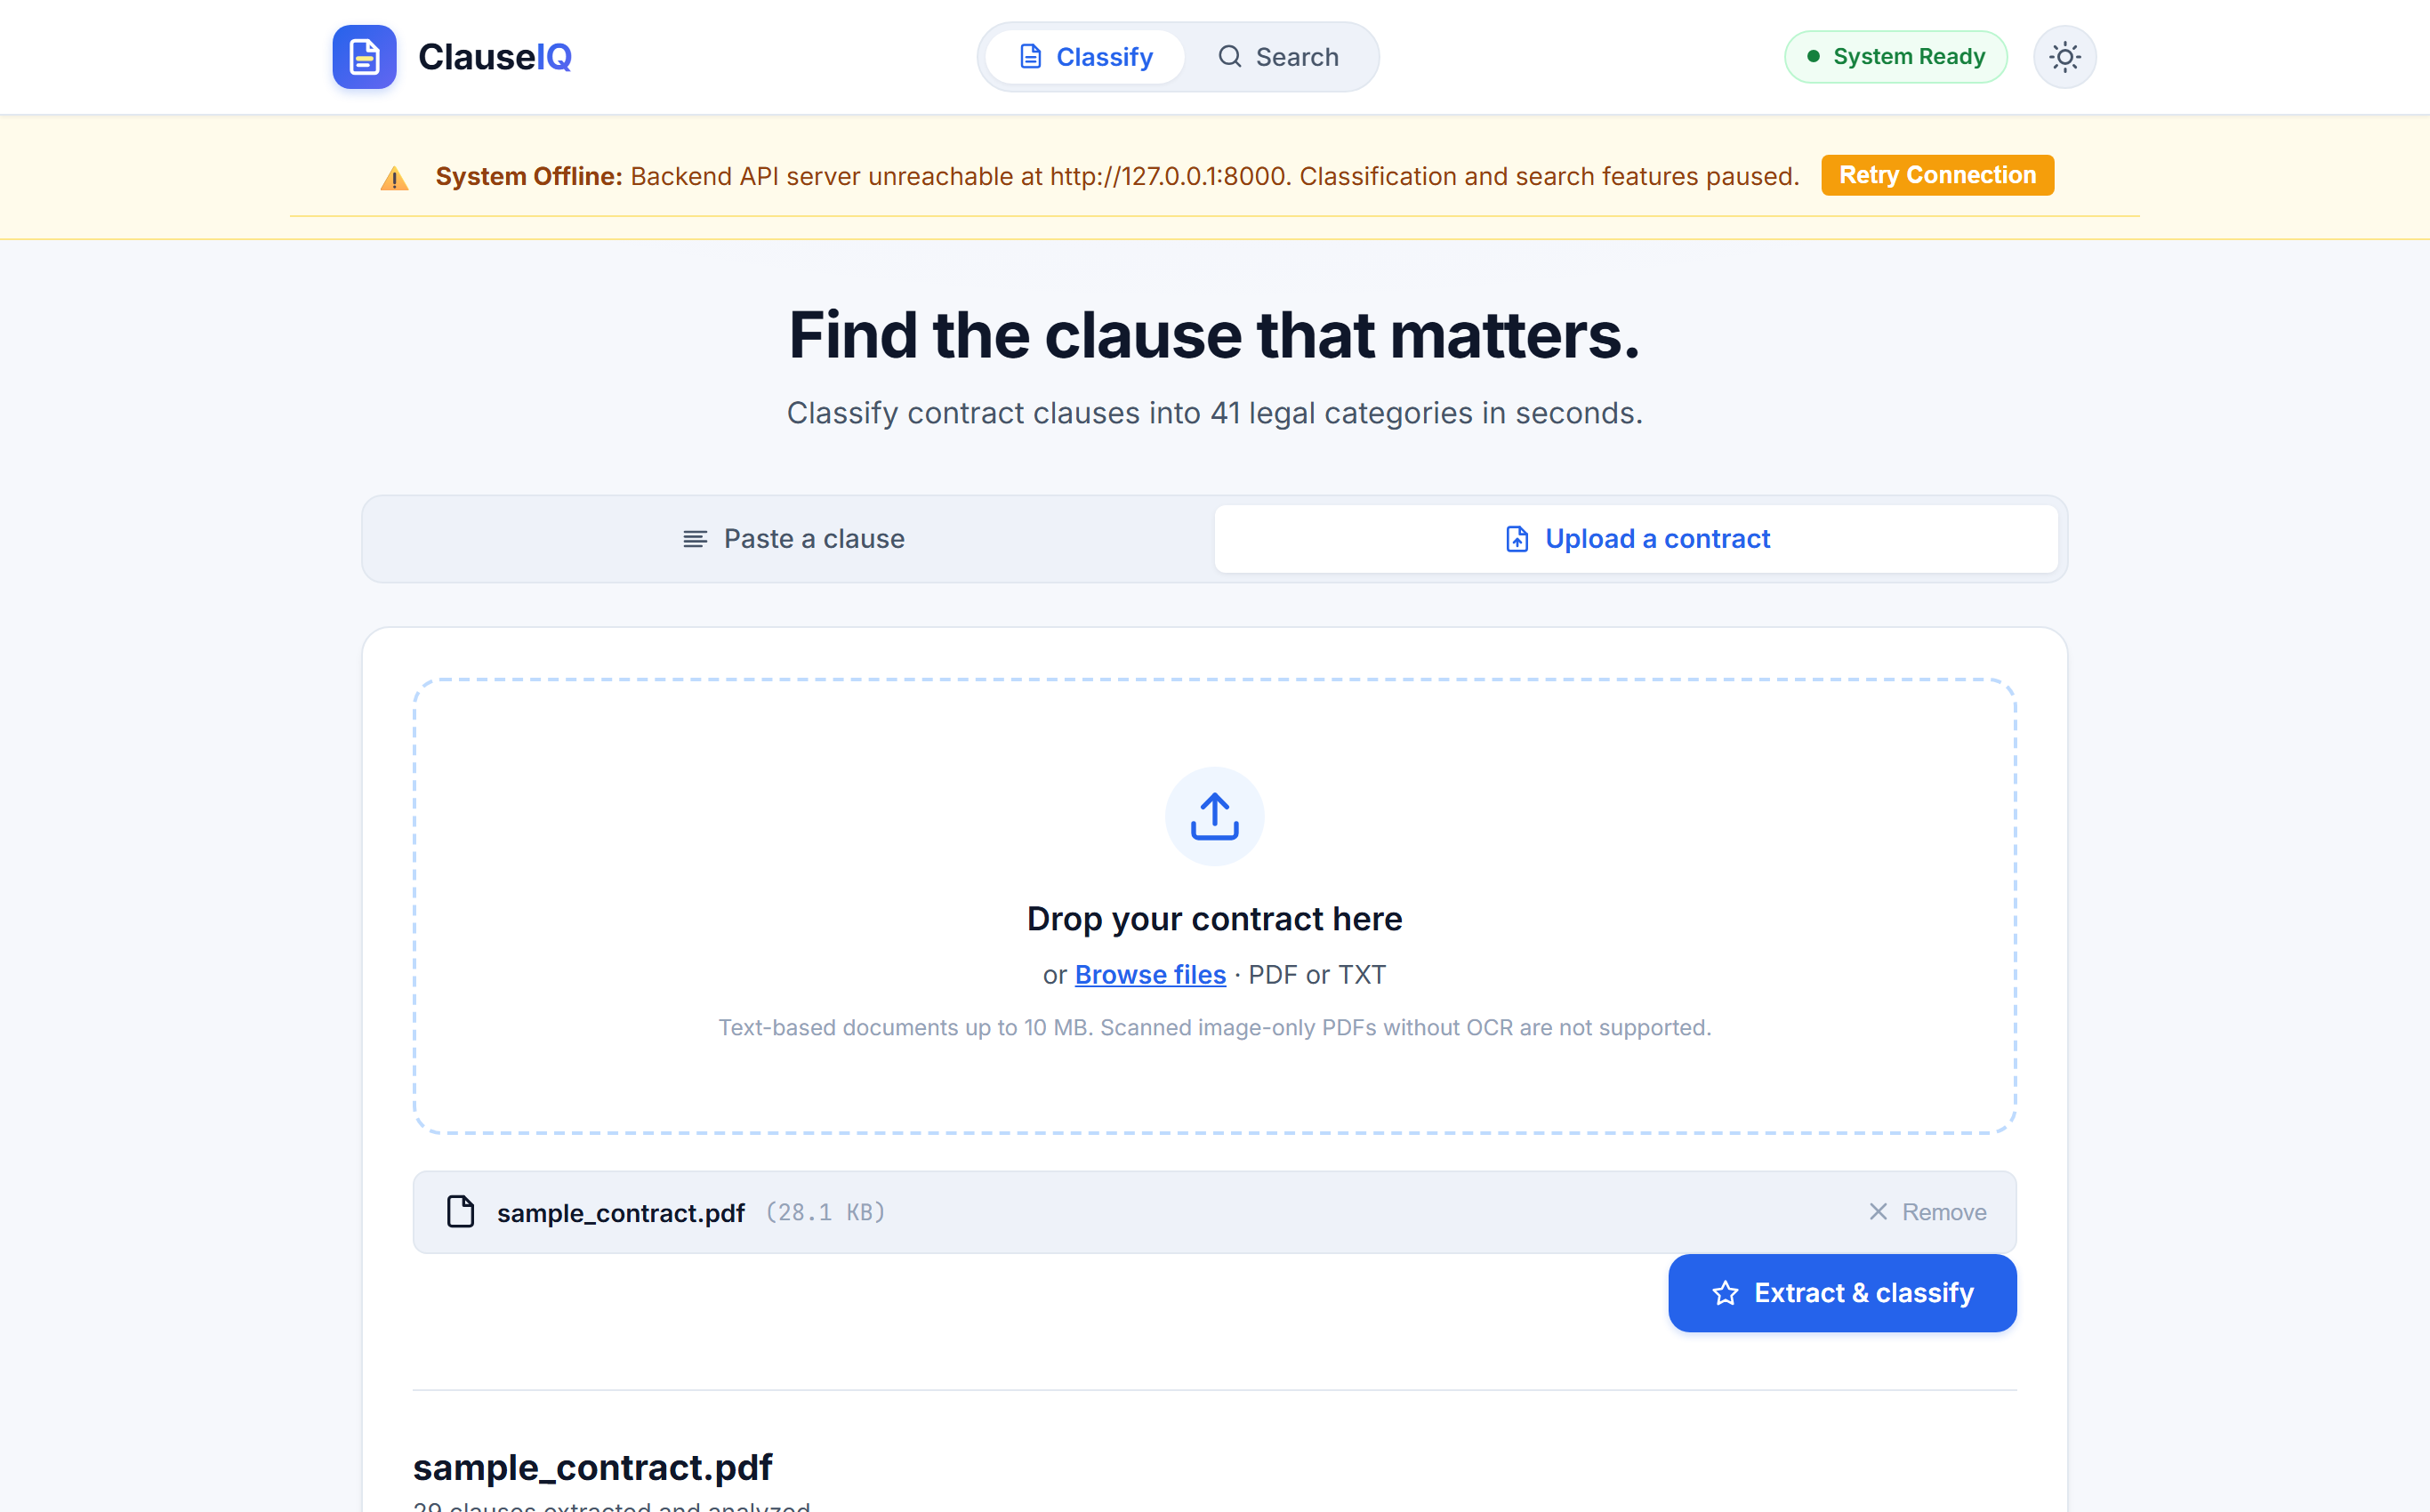
\includegraphics[width=0.88\textwidth]{figures/ui/ui_07_offline_banner.png}
\caption{User interface: Offline banner alerting the user when the backend API service is disconnected}\label{fig:ui_offline_banner}
\end{figure}

Figure~\ref{fig:ui_api_docs} displays the interactive FastAPI OpenAPI documentation interface accessible at \texttt{/docs}. The Swagger UI provides an interactive specification of all seven backend endpoints, including schemas and interactive trial calls.

\begin{figure}[!htbp]
\centering
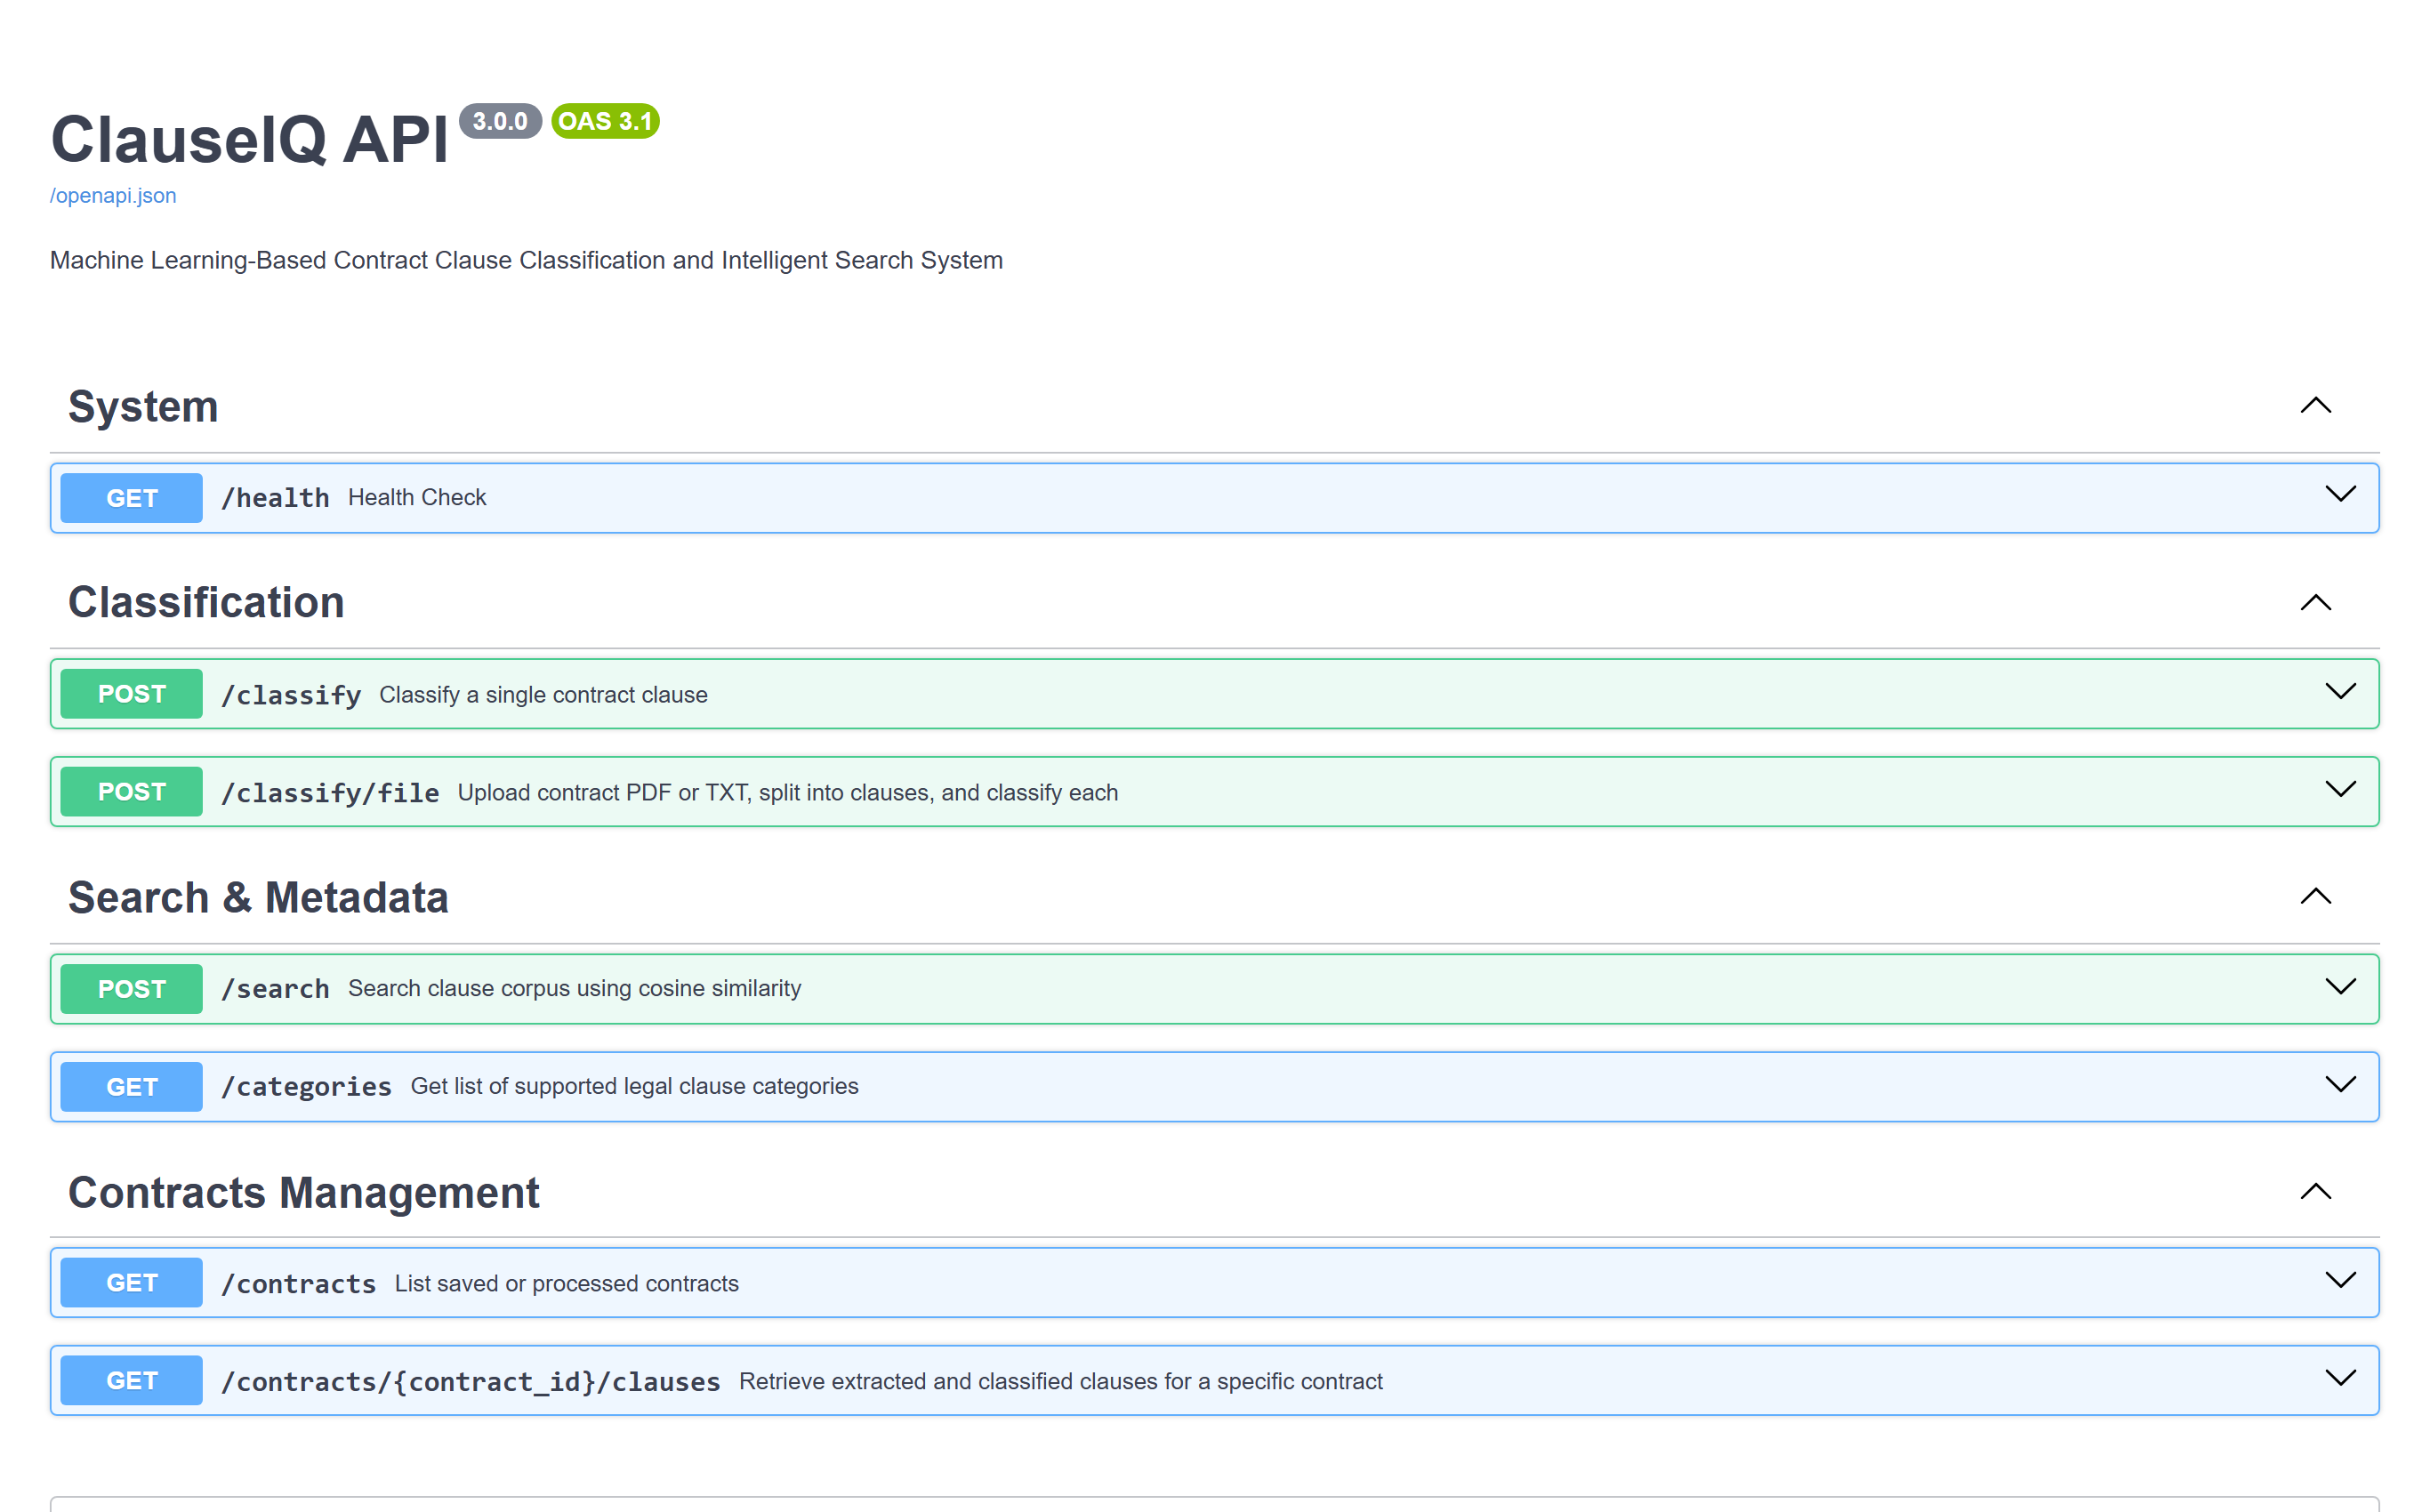
\includegraphics[width=0.80\textwidth]{figures/ui/ui_08_api_docs.png}
\caption{User interface: Interactive FastAPI Swagger documentation (\texttt{/docs}) detailing all REST endpoints}\label{fig:ui_api_docs}
\end{figure}


% Chapter 7: Git History
\chapter{Git history}
\label{ch:git_history}

The development lifecycle of the ClauseIQ system has been tracked using the Git distributed version control system and hosted on GitHub. This chapter documents the chronological progression of commits across the active development branch, reflecting the iterative evolution from initial exploratory data analysis through baseline machine learning, feature optimization, backend API hardening, and frontend user interface deployment.

\paragraph*{Repository overview}
The repository configuration and version control metadata for ClauseIQ are:
\begin{itemize}
    \item Repository URL: \url{https://github.com/Farhan-kalady/ClauseIQ.git}
    \item Active development branch: \texttt{feature/complete-clauseiq}
    \item Total development commits: 13 verified commits
    \item Tracking period: August 7, 2026 to October 19, 2026
\end{itemize}

\paragraph*{Commit progression log}
Table~\ref{tab:git_history} provides the complete chronological record of commits on the active development branch, generated directly from the repository's version control log via \texttt{git log}.

% Auto-generated by scripts/make_numbers.py
\begin{longtable}{p{2.0cm} p{2.2cm} >{\raggedright\arraybackslash}p{10.2cm}}
\toprule
\textbf{Commit Hash} & \textbf{Date} & \textbf{Commit Summary Message} \\
\midrule
\endfirsthead
\multicolumn{3}{c}{{\bfseries Table \thetable\ continued from previous page}} \\
\toprule
\textbf{Commit Hash} & \textbf{Date} & \textbf{Commit Summary Message} \\
\midrule
\endhead
\midrule
\multicolumn{3}{r}{{Continued on next page}} \\
\bottomrule
\endfoot
\bottomrule
\caption{Repository version control commit history (verified on active branch)}\label{tab:git_history}\\
\endlastfoot
\texttt{ef1acc6} & 2026-10-19 & docs: Phase 5 end-to-end verification, documentation alignment, and project completion \\
\texttt{9e4f56d} & 2026-10-19 & feat(ui): complete Phase 4 frontend matching DesignDoc, restore verified clause splitter, and add deterministic color tokens \\
\texttt{6debd61} & 2026-10-19 & feat(api): Phase 3 backend completion - upload hardening, scoped search, atomic persistence, contract read endpoints, and cleaned dependencies \\
\texttt{2f22a3b} & 2026-10-19 & feat(ml): complete Phase 2 model improvements with hybrid word-char features, error analysis, and final benchmarks \\
\texttt{40433b8} & 2026-10-19 & feat(eval): complete Phase 1 baseline reproducibility and Split A/B trustworthy evaluation \\
\texttt{56d49d2} & 2026-10-19 & docs: complete Step 0 audit and create feature branch \\
\texttt{b9112e7} & 2026-10-11 & feat: complete pre-submission audit, Supabase schema idempotency, and env configuration \\
\texttt{80a7ee6} & 2026-10-08 & feat(sprint-3): complete full-stack integration and deployment with FastAPI, React frontend, Supabase schema, and 41 verified tests \\
\texttt{07e65a6} & 2026-09-05 & Complete Sprint 1 core ML pipeline \\
\texttt{b5dcd46} & 2026-09-04 & Project structure setup for Sprint 1 \\
\texttt{2a3b196} & 2026-08-19 & Readme File Added \\
\texttt{c7e9720} & 2026-08-19 & Report added \\
\texttt{b651e16} & 2026-08-07 & DataSet Exploration Completed \\
\end{longtable}


The version history demonstrates the structured development milestones of the project:
\begin{enumerate}
    \item Foundational phase (commits \texttt{b651e16} to \texttt{b5dcd46}): Initial exploratory data analysis on the CUAD corpus, directory structure configuration, baseline documentation, and project scoping.
    \item Core machine learning phase (commit \texttt{07e65a6}): Implementation of text cleaning routines, stratified train/test partitioning, unigram/bigram TF-IDF vectorization, and multi-model benchmarking.
    \item Full-stack integration phase (commits \texttt{80a7ee6} to \texttt{b9112e7}): Construction of the FastAPI backend, implementation of the React single-page interface, Supabase PostgreSQL schema migration, and initial automated test suites.
    \item System optimization and hardening phase (commits \texttt{56d49d2} to \texttt{ef1acc6}): Trustworthy leakage-safe grouped split evaluation (Split~B), hybrid word-plus-character feature engineering, probability calibration analysis, API upload security hardening, scoped contract search, and end-to-end verification.
\end{enumerate}

Figure~\ref{fig:github_commit_history} presents the verified commit history interface of the ClauseIQ repository on GitHub.

\begin{figure}[htbp]
\centering
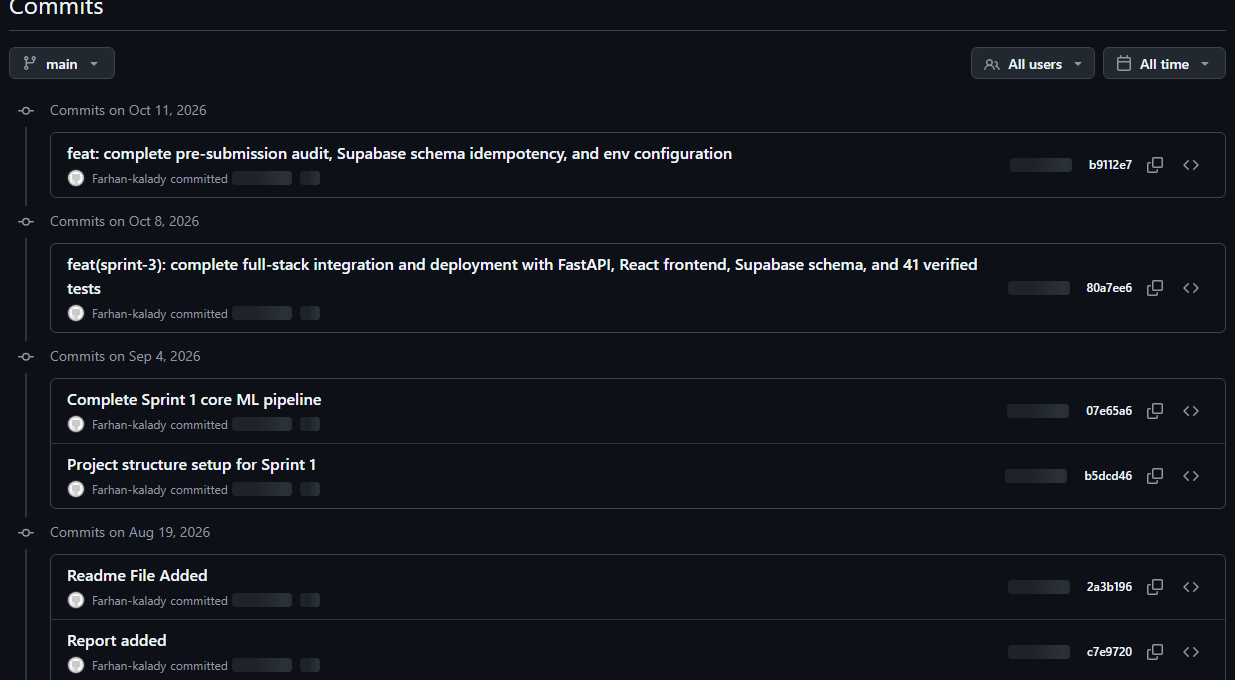
\includegraphics[width=0.96\textwidth]{figures/git_commit_history.png}
\caption{Verified GitHub repository commit history for ClauseIQ}\label{fig:github_commit_history}
\end{figure}

The source code and commit history are publicly accessible at the official repository: \url{https://github.com/Farhan-kalady/ClauseIQ.git}.



% Chapter 8: Conclusions
\chapter{Conclusions}
\label{ch:conclusions}

This project successfully researched, designed, evaluated, and deployed ClauseIQ---an end-to-end, machine learning-based contract clause classification and intelligent search prototype system engineered to assist in the triage of complex commercial agreements. By leveraging the expert-annotated Contract Understanding Atticus Dataset (CUAD), the project established a reliable, deterministic, and privacy-preserving legal technology pipeline.

\paragraph*{Summary of technical achievements}
The core technical milestones achieved in this project comprise:
\begin{enumerate}
    \item Comprehensive corpus validation: Processed, cleaned, and validated \TotalClauses{} clause instances originating across \TotalContracts{} SEC EDGAR commercial contracts, preserving all \NumClasses{} standardized legal categories without discarding low-frequency classes.
    \item Domain-specific feature engineering: Empirically demonstrated that standard stopword removal degrades legal text classification, while NLTK WordNet lemmatization and hybrid representation (uniting 25,000 word n-grams with 15,000 character-within-word-boundary n-grams) elevate discriminative capability, achieving a 5-fold cross-validation Macro-F1 of 0.6865.
    \item Rigorous leakage-aware benchmarking: Evaluated four classical architectures across two distinct partitioning protocols. On the standard stratified split (Split~A), the final Multinomial Logistic Regression model achieved \FinalSplitAAcc{} Accuracy, \FinalSplitAMacroFScore{} Macro-F1, and \FinalSplitAWeightedFScore{} Weighted-F1. On the contract-grouped split with zero parent agreement overlap (Split~B), the model achieved \FinalSplitBAcc{} Accuracy and \FinalSplitBMacroFScore{} Macro-F1, demonstrating robust cross-contract generalization.
    \item Empirical probability calibration: Reduced Expected Calibration Error (ECE) from 0.2822 down to \FinalSplitAECE{}. Over 53\% of predictions achieved High Confidence ($\ge 0.50$), delivering an empirical precision of \FinalSplitBHighConfPrec{} on unseen agreements.
    \item High-precision semantic retrieval: Constructed a TF-IDF and Cosine Similarity search engine achieving Precision@1 of 0.80 and Precision@5 of 0.88 across benchmark legal queries, operating with measured mean retrieval latency of approximately 100~ms across 12,204 clauses.
    \item Full-stack production delivery: Encapsulated the machine learning models within an asynchronous FastAPI service, integrated a Supabase PostgreSQL persistence schema prototype for audit logging, and developed an intuitive React.js single-page interface verified through 45 passing automated tests.
\end{enumerate}

\paragraph*{System boundaries and operational truthfulness}
To maintain ethical and technical transparency, the operational boundaries of ClauseIQ are emphasized:
\begin{itemize}
    \item Classical statistical paradigm: ClauseIQ is deliberately built upon classical machine learning algorithms. The deployed system does not utilize deep neural networks, transformer architectures, or generative Large Language Models. This design ensures rapid execution (mean single-clause inference latency of 6.58~ms), deterministic reproducibility, low compute overhead, and complete data privacy.
    \item Decision-support scope: ClauseIQ functions solely as an assistive legal technology prototype. It does not provide legal advice, generate binding legal opinions, or replace qualified legal counsel.
    \item Semantic ambiguity ceilings: Error analysis revealed that misclassifications are concentrated within reciprocal category pairs (such as Agreement Date vs Effective Date, and Cap On Liability vs Uncapped Liability) where conflicting legal concepts appear within the same sentence. Legal human-in-the-loop oversight remains essential for these provisions.
    \item Authentication and hosting: In its present implementation, ClauseIQ executes locally or within private networks; user authentication and cloud hosting are not configured.
\end{itemize}


% Chapter 9: Future Scope
\chapter{Future scope}
\label{ch:future_scope}

While the current ClauseIQ implementation provides a robust, validated, and low-latency classical machine learning platform, several valuable avenues for architectural enhancement and functional expansion have been identified for future research and development cycles.

\paragraph*{Optical character recognition (OCR) for scanned agreements}
The current document ingestion pipeline utilizes PyMuPDF, which requires uploaded PDF contracts to contain embedded digital text layers. In enterprise legal archives, a substantial fraction of legacy agreements exist solely as scanned raster images or degraded facsimile copies. Integrating an upstream, open-source Optical Character Recognition (OCR) engine---such as Tesseract OCR or EasyOCR---would allow ClauseIQ to process scanned contracts seamlessly. Future engineering would focus on combining high-speed image binarization, skew correction, and noise removal prior to text extraction.

\paragraph*{Hierarchical two-stage classification}
As evidenced by the error analysis in Chapter~\ref{ch:results_and_discussion}, the majority of classification errors occur between closely related, semantically entangled category pairs (for instance, \textit{Cap On Liability} versus \textit{Uncapped Liability}, or \textit{License Grant} versus \textit{Non-Transferable License}). A flat 41-class softmax classifier must distribute probability mass across all categories simultaneously.

A promising future direction is the design of a hierarchical two-stage classification framework:
\begin{enumerate}
    \item Stage 1 (macro-level covenant routing): A coarse-grained linear classifier maps the clause into one of 8 broad legal families (e.g., \textit{Liability Allocation}, \textit{Intellectual Property Rights}, \textit{Term and Termination}, \textit{Restrictive Covenants}, \textit{Jurisdiction and Dispute Resolution}).
    \item Stage 2 (fine-grained subtype specialization): A dedicated, specialized binary or multi-class discriminator trained specifically on targeted discriminative tokens distinguishes between confusable subtypes within that specific family.
\end{enumerate}

\paragraph*{Domain-adapted deep learning and hybrid embeddings}
\textit{Explicit Scope Boundary:} Deep neural networks and Large Language Models are explicitly out of scope for the current ClauseIQ release. However, as an avenue of future academic inquiry, exploring hybrid architectures offers substantial potential:
\begin{itemize}
    \item Domain-specific transformer representations: Evaluating pre-trained legal encoders---such as LegalBERT~\cite{chalkidis2020legal}---fine-tuned specifically on the CUAD corpus to capture contextual dependencies that extend beyond n-gram windows.
    \item Hybrid dense-sparse information retrieval: Combining the lexical precision of BM25 / TF-IDF sparse vectors with dense vector embeddings (e.g., dense passage retrieval) to capture both exact statutory phrasing and conceptual paraphrasing.
\end{itemize}

\paragraph*{Enterprise security and deployment scaling}
To facilitate commercial deployment within multi-tenant enterprise environments, future engineering milestones include:
\begin{itemize}
    \item Authentication and role-based access control (RBAC): Implementing OAuth2 / OpenID Connect single sign-on (SSO) with fine-grained access permissions, ensuring segregation between corporate legal entities.
    \item Containerization and cloud orchestration: Packaging the FastAPI backend and React frontend into standardized Docker container images orchestrated via Kubernetes or serverless container platforms.
    \item Active learning feedback loop: Implementing an attorney review interface where legal practitioners can correct borderline or low-confidence classifications, feeding anonymized verified samples back into periodic retraining pipelines.
\end{itemize}


% Chapter 10: Appendix
\chapter{Appendix}
\label{ch:appendix}

\section{Minimum software requirements}
\label{sec:appendix_software}

\begin{table}[htbp]
\centering
\begin{tabular}{|p{4.5cm}|p{10.5cm}|}
\hline
Component & Requirement \\
\hline
Operating system & Windows 10 or later, Linux (Ubuntu 20.04+), or macOS \\
\hline
Programming language & Python 3.10 or later, Node.js 18 or later \\
\hline
Data handling & Pandas, NumPy \\
\hline
Machine learning & Scikit-learn (LinearSVC, Logistic Regression, TF-IDF Vectorizer) \\
\hline
Natural language processing & NLTK (Tokenization, WordNet Lemmatizer, Stopwords) \\
\hline
Document processing & PyMuPDF (fitz) for PDF clause extraction \\
\hline
Web framework & FastAPI (REST API Backend), React.js with Vite (Frontend) \\
\hline
Database & Supabase (PostgreSQL) cloud database \\
\hline
Model storage & Joblib \\
\hline
Development environment & VS Code or any modern code editor \\
\hline
Web browser & Any modern browser (Chrome, Edge, Firefox) \\
\hline
Version control & Git \\
\hline
\end{tabular}
\caption{Minimum software requirements}\label{tab:appendix_software}
\end{table}

\section{Minimum hardware requirements}
\label{sec:appendix_hardware}

\begin{table}[htbp]
\centering
\begin{tabular}{|p{4.5cm}|p{10.5cm}|}
\hline
Component & Requirement \\
\hline
Processor & Dual-core CPU, 2 GHz or higher (Quad-core recommended) \\
\hline
Memory (RAM) & 4 GB minimum (8 GB recommended for model training) \\
\hline
Storage & 2 GB of free disk space (4 GB recommended for dataset and models) \\
\hline
GPU & Not required (CPU-based inference and feature extraction) \\
\hline
Internet & Required for downloading dependencies, API serving, and Supabase cloud synchronization \\
\hline
\end{tabular}
\caption{Minimum hardware requirements}\label{tab:appendix_hardware}
\end{table}


% Chapter 11: References
\chapter{References}
\label{ch:references}

\begingroup
\renewcommand{\chapter}[2]{}% Suppress redundant unnumbered chapter heading generated by thebibliography
\begin{thebibliography}{10}

\bibitem{quevedo2024legal}
E.~Quevedo Caballero, T.~{\v{C}}ern{\'y}, A.~Rodriguez, P.~Rivas, J.~Yero, K.~Sooksatra, and D.~Taibi,
``Legal Natural Language Processing From 2015 to 2022: A Comprehensive Systematic Mapping Study of Advances and Applications,''
\textit{IEEE Access}, vol.~12, pp.~145286--145317, 2024, doi: 10.1109/ACCESS.2024.3414967.

\bibitem{siino2025exploring}
M.~Siino, M.~Falco, D.~Croce, and P.~Rosso,
``Exploring LLMs Applications in Law: A Literature Review on Current Legal NLP Approaches,''
\textit{IEEE Access}, vol.~13, pp.~18253--18276, 2025, doi: 10.1109/ACCESS.2025.3533217.

\bibitem{kutbi2023named}
M.~Kutbi,
``Named Entity Recognition Utilized to Enhance Text Classification While Preserving Privacy,''
\textit{IEEE Access}, vol.~11, pp.~117576--117581, 2023, doi: 10.1109/ACCESS.2023.3325895.

\bibitem{hendrycks2021cuad}
D.~Hendrycks, C.~Burns, A.~Chen, and S.~Ball,
``CUAD: An Expert-Annotated NLP Dataset for Legal Contract Review,''
in \textit{Proceedings of the Thirty-fifth Conference on Neural Information Processing Systems (NeurIPS 2021) Track on Datasets and Benchmarks}, 2021.

\bibitem{pedregosa2011scikit}
F.~Pedregosa \textit{et~al.},
``Scikit-learn: Machine Learning in Python,''
\textit{Journal of Machine Learning Research}, vol.~12, pp.~2825--2830, 2011.

\bibitem{bird2009natural}
S.~Bird, E.~Klein, and E.~Loper,
\textit{Natural Language Processing with Python}. Sebastopol, CA: O'Reilly Media, 2009.

\bibitem{guo2017calibration}
C.~Guo, G.~Pleiss, Y.~Sun, and K.~Q. Weinberger,
``On Calibration of Modern Neural Networks,''
in \textit{Proceedings of the 34th International Conference on Machine Learning (ICML)}, vol.~70, pp.~1321--1330, 2017.

\bibitem{manning2008introduction}
C.~D. Manning, P.~Raghavan, and H.~Sch{\"u}tze,
\textit{Introduction to Information Retrieval}. Cambridge, UK: Cambridge University Press, 2008.

\bibitem{chalkidis2020legal}
I.~Chalkidis, M.~Fergadiotis, P.~Malakasiotis, N.~Aletras, and I.~Androutsopoulos,
``LEGAL-BERT: The Muppets Straight Out of Law School,''
in \textit{Findings of the Association for Computational Linguistics: EMNLP 2020}, pp.~2898--2904, 2020.

\bibitem{salton1988term}
G.~Salton and C.~Buckley,
``Term-Weighting Approaches in Automatic Text Retrieval,''
\textit{Information Processing \& Management}, vol.~24, no.~5, pp.~513--523, 1988.

\end{thebibliography}
\endgroup


\end{document}
